%\documentclass[11pt,a4paper,twoside,openright]{book}
\documentclass{book}
\usepackage{amsmath}
\usepackage{fullpage}
\usepackage[left=1cm,right=1cm,top=2cm,bottom=2cm]{geometry}
\usepackage[usenames,dvipsnames]{color}
\usepackage{graphicx}
\usepackage{float}
%\usepackage{booktabs}
\usepackage{multirow}
\usepackage{wrapfig}							% allows wrapping text around figures
%\usepackage{cite}
%\usepackage[labelfont=bf]{caption}
\usepackage{titlesec}
\titleformat{\section}[block]{\large\bfseries}{\thesection}{1em}{}
\usepackage{framed}
\usepackage{multicol}
\usepackage{hyperref}
\usepackage{enumerate}
\usepackage{enumitem}
\usepackage{setspace}

%\setlength{\marginparwidth}{0pt}

 % Define commands to assure consistent treatment throughout document
% \newcommand{\eqnref}[1]{(\ref{#1})}
 \newcommand{\class}[1]{\texttt{#1}}
 \newcommand{\package}[1]{\texttt{#1}}
 \newcommand{\file}[1]{\texttt{#1}}
 \newcommand{\BibTeX}{\textsc{Bib}\TeX}
\renewcommand{\thesection}{\arabic{section}.}
\renewcommand{\thesubsection}{{\thesection}\Alph{subsection}.}
\renewcommand{\thesubsubsection}{\alph{subsubsection}.}

\def\beq{\begin{equation}}
\def\eeq{\end{equation}}
\def\beqn{\begin{matrix}}
\def\eeqn{\end{matrix}}

\begin{document}

\thispagestyle{empty}
%\vspace*{1 mm}
\begin{center}
\begin{LARGE}{\bf NUMERICAL METHODS FOR UNIVERSITY OF SOUTH ALABAMA}\end{LARGE}\\
\large
\vspace{22 mm}
\begin{singlespace}
   A Brief Textbook Presented to the \\ 
   Student Body of the University of South Alabama \\
\vspace{22 mm}
   by\\
\vspace{22 mm}
  Carlos Montalvo \\
\vspace{22 mm}
For use in Mechanical Analysis I \& II \\
\vspace{82 mm}
\end{singlespace}
{\itshape University of South Alabama}
{\bf Copyright $\copyright$ Carlos Jos\'{e} Montalvo 2015}
\end{center}


\tableofcontents

%\input{../Syllabus/Syllabus}

%\input{../Syllabus/ABET_Criteria}

%
\section{Fun Icebreakers(Homework 1)} 

These icebreakers will be completed on the first day of class using
polleverywhere.com

\begin{enumerate}

\item Name TWO things you hate to see in lecture.


\item How good are you at mathematics?
  
  \begin{enumerate}
    \item I am Carl Gauss traveling from the past.
    \item I took Calculus.
    \item I slept through Calculus
    \item 2+2=5
  \end{enumerate}

\item Ok prove it. Solve this equation. 

  \begin{equation}\nonumber
    \int\limits_{-1}^1\sqrt{1-x^2}dx
  \end{equation}

\item How good are you are computers?

  \begin{enumerate}
    \item Compute what?
    \item I can check my Facebook
    \item I know how to write a document in WORD
    \item I can install programs
    \item I have created a computer program (MATLAB, Python, etc...)
    \item I wrote the internet
  \end{enumerate}

\item Ok prove it. out = myfunc(5). What is out?

function out = myfunc(N)

out = 0

for idx = 1:N

out = out + idx

end

\item True False

  \begin{enumerate}
     \item This class is hard?
     \item Computers are evil?
     \item There is no such thing as bad code?
     \item You need to be good at computers to pass this class?
     \item Working problems out by hand is becoming obsolete?
  \end{enumerate}

\end{enumerate}


%\section{GAME DAY!!}

Class Breaks into Groups. Winning group gets a prize

\begin{enumerate}

\item Answer the following questions. You only have 2 minutes to write as
many as possible

\begin{enumerate} 
  \item Name as many famous mathematicians as you can
  \item Name as many physicists as you can
  \item Name as many philosophers as you can
  \item Name as many programming languages as you can
  \item Name as many transcendental functions as you can
  \item Name as many solids and shapes as you can
\end{enumerate}

\item MATLAB Jeopardy. Students stay in their groups and they have to try
  and answer the questions I have in a PDF. Examples
  include adding all the primes from 1 to 1000 or computing your age
  in days accounting for leap year. I have a text file showing
  different questions for them to complete. Each problem must be
  completed using MATLAB. Each problem can be solved with 5 lines of
  code or less.

\end{enumerate}




%%%%GROUP 1 - MATLAB

\section{INTRODUCTION TO MATLAB}

\subsection{Basics of MATLAB - Palm - Chapter 1}

\begin{enumerate}

\item \textbf{MATLAB(Current Directory, Workspace, Command Window, File)
interface}

When you double click MATLAB you will have a number of windows
present. The configuration of all windows in your MATLAB version may
be different but the names are all the same.

\begin{figure}[htb]
  \begin{center}
    \includegraphics[height=0.55\textwidth,width=0.8\textwidth]{Graphics/MATLAB}
  \end{center}
\end{figure}

The very top of the MATLAB window is our toolbar. It has similar
buttons such as File, Edit, etc. Below this is your current
directory. This lists the current folder that you are operating
in. The window in the upper right is the Current Directory as well
which lists all the files currently in the folder. In this example I
have an error.jpg file, a mypi.m and test\_pi.m file. Note that a .jpg
is a picture file and a .m file is a MATLAB script file. The window
directly to the right is the Workspace. This lists all the current
variables in the workspace. The lower left window is my Command
History. It contains the history of all of my inputs into the Command
Window. The command window is where I can use MATLAB like a
calculator. If I type the following command

$>>$ x = 1

into the command window, MATLAB will create a variable 1 and save it
into x. Everytime I type in x it will now use 1 as the value. Thus, if
I type in 

$>>$ y = 2*x

the variable y will be evaluated as 2*x where x = 1 thus 2*1 = 2 and y
will be 2.

\item \textbf{Order of operations}

MATLAB works just like your calculator does. Thus, you need to make
sure parentheses are in the correct spot. For example

$>>$ x = 1/(2+1) 

will set x = to one third. However, 

$>>$ x = 1/2+1

will set x = 0.5 + 1 = 1.5. Try this in MATLAB to see the
difference. It is important to remember PEMDAS (Parentheses,
Exponents,Multiplication/Division, Addition/Substraction) That is,
MATLAB evaluates those operators in that order.

\item \textbf{Learn format of output}

There may be times when you need to see more than 4 significant
digits. For example,

$>>$ x = sqrt(2)

will output x = 1.4142. However it may be beneifical to see more
significant digits. To do that simply type

$>>$ format long g

into MATLAB. Then when you type 'x' into MATLAB you should see 13
digits. To return to normal output simply type

$>>$ format short g

\item \textbf{ What variables do I have?}

Sometime through your coding you will have alot of variables in your
workspace. For example it you type

$>>$ x = 2

$>>$ y = 2*x

$>>$ z = x\textrm{\^}2

In order to see all of your variables you can simply type 

$>>$ whos

into MATLAB. This will output all variable names in your workspace,
their size, the number of bytes they are taking up and the class which
is also known as type. Another way to see the current variables is to
simply look at the workspace window.

\item \textbf{ Variable Types}

There are numerous types of variables that MATLAB can handle. Think of
them as different currencies. For example I could give you a number
which is known as a double

$>>$ x = 42

or I could give you a set of characters known as a char.

$>>$ s = 'Hello World'

If I then type in 

$>>$ whos 

into MATLAB I see that I have a variable x with a size of 1x1, using 8
bytes, and a class of double. I also will have a variable s with a
size of 1x11, and a class of char. The size of s is 1x11 because I
have 11 characters in the variable. The space is included. The number
of bytes is equal to 2*11 or 22. That is because MATLAB needs 2 bytes
for every letter and thus needs 22 bytes to represent that number. A
double always needs 8 bytes. That is, the number 42 needs 8 bytes, the
number 6789 needs 8 bytes. The name double comes from the fact that
numbers are converted to binary which is of base 2. If I wish to
convert variables from one type to another I use the functions num2str
and str2num. 

$>>$ x = 1

$>>$ y = num2str(x)

The code above will convert the variable x to a string and save it in
y. Note that if you type whos into MATLAB x will still be a double but
y will be a string. Try using str2num to see what happens.

Note that the reason why MATLAB uses 2 bytes per character is because
it uses the unicode UTF-16 standard. Remember that 2 bytes is 16 bits
hence UTF-16. How many characters can UTF-16 represent? Check out the
entire list here.

http://www.fileformat.info/info/charset/UTF-16/list.htm

Obviously there are other formats such as UTF-7 and UTF-8 which stand
for 7 and 8 bit respectively. They all have their strengths and
weaknesses. 

\item \textbf{Scripting}

Alot of times you will have to compute something such as the number of
seconds in a day. This can be easily accomplished by typing.

$>>$ seconds\_min = 60

$>>$ seconds\_hour = 60*seconds\_min

$>>$ seconds\_day = 24*seconds\_hour

However, if you make a mistake you will have to clear everything

$>>$ clear

and start over. This can be very tedious. Thus scripting was
invented. 

\begin{enumerate}

\item \textbf{ Open a File...}

To open a file you can simply click File $\rightarrow$ New
$\rightarrow$ Blank M-File. Once the file is open you must save the
file by clicking File $\rightarrow$ Save. You can also type

$>>$ edit filename.m

into MATLAB and it will create a file called filename.m. If you then
return to the MATLAB window notice that you will have the file
filename.m in your current directory. If you type

$>>$ ls

into MATLAB you should also see your filename displayed there as
well. With the script open you can then create a script.

\item \textbf{Example Script}

Below is a simple script calculating the number of seconds in a
day. The first three lines clears the workspace, the command window
and closes all open figures. Note that the \% is a comment that can be
used to make notes in your script.

\begin{framed}

clear 

clc

close all

\%\%\%This is a comment

seconds\_min = 60

seconds\_hour = 60*seconds\_min

seconds\_day = 24*seconds\_hour

\end{framed}

\item \textbf{ Execute Script}

There are three ways to execute a script. 

\begin{enumerate}
  
\item Hit the play button from the top of the editor
\item Hit F5 on the keyboard
\item Type 

$>>$ filename 

in the command window. When you type filename in the command window,
MATLAB will search for a file called filename.m and execute the
contents of the script. If the file does not exist, MATLAB will throw
an error.

\end{enumerate}

\end{enumerate}

\item \textbf{Directories}

Further along you may download a file from the internet and open it in
MATLAB. When you do this the file will be opened in a editor in
MATLAB. However, when you attempt to run this script, MATLAB will ask
you whether or not you would like to change the current directory. If
you do this the current directory at the top toolbar will change to
the location of the file you just downloaded. Note that if you then
run another file you will have to change the directory again. I urge
you to try and organize your files such that everything makes
intuitive sense.

\item \textbf{Help!}

If at any point you ever lose your way simply type 

$>>$ help 

into MATLAB. If you know of a function but you forget what it does or
how to use it simply type

$>>$ help $<$variable name$>$

for example

$>>$ help num2str

will list what num2str does and how to use it.

\item {\bf Functions Learned}

whos

clear

clc

format long g

ls

num2str, str2num

disp

\end{enumerate}




\subsection{Arrays - Palm - Chapter 2}

\begin{enumerate}

\item \textbf{Inputting Arrays}

Whenever you type a variable into MATLAB 

$>>$ x = 1

MATLAB will create an array. The variable x currently is a 1x1
array. That is it has 1 row and 1 column. It is possible however to
create a vector of numbers.

$>>$ x = [1 2 3 4]

This will create a vector with 1 row and 4 columns. It is possible to
make the same vector with only 1 column by using a semicolon.

$>>$ x = [1 ; 2 ; 3 ; 4]

This will create a variable with 4 rows and 1 column. It is also
possible to create a column vector by using the transpose value.

$>>$x = [1 2 3 4]'

The ' will transpose the vector. In order to create a matrix you
simply combine the semicolons and spaces.

$>>$ A = [1 2 ; 3 4]

This will create a 2x2 matrix. It is also possible to create rules for
vectors. For example, say you want all even number from 2 to 100. This
can be accomplished by using the form

\item \textbf{Linspace vs. Increment}

{\it start:increment:end}

$>>$ x = 2:2:100

The line above will start at 2, increment by 2 and stop when it hits
100. You can also use the linspace command which uses the form

{\it linspace(start,end,number of elements)}

$>>$ x = linspace(1,10,5)

The line above will create a vector that starts at 1 and end at 10 but
contains 5 elements.

\item \textbf{Length Command}

$>>$ L = length(x)

Length will compute the number of elements in the vector. In this case
L will be equal to 5. If you type whos in MATLAB you will see that x
is a vector 1x5 and L is a 1x1 but its value is 5.

\item \textbf{ Creating Empty Matrices}

To create empty matrices you may use the zeros() and ones() command.

$>>$ A = zeros(5,3)

The line above will create a matrix of zeros with 5 rows and 3
columns. 

Note that adding matrices is very simple. 

$>>$ B = zeros(5,3) + 5

will create a matrix of zeros with 5 rows and 3 columns and then add
the number 5 to every element in the matrix.

\item \textbf{Add/Substract and Multiply/Divide}

$>>$ C = A + B

this will then add the contents of A to B. Similar results are seen
for substraction. Multiplication is tricky. The following line will
throw an error.

$>>$ C = A*B $\leftarrow$ ERROR

The reason is that A is a 5x3 and B is a 5x3. As such the inner matrix
dimensions do not match.

$>>$ x = [1 ; 3]

$>>$ A = [1 2 ; 4 5]

$>>$ b = A*x

the lines above are totally valid because x is a 2x1 and A is a 2x2
thus b is a 2x1. Type in whos to verify. 

\item \textbf{Dot Operator}

It may be beneficial to compute the square of the numbers from say 1
to 10.

$>>$ x = 1:1:10

will create the numbers from 1 to 10 incrementing by 1.

$>>$ x = x\textrm{\^}2 $\leftarrow$ ERROR

This again will throw an error because x is a 1x10. A 1x10 times a
1x10 does not have the inner matrix dimensions that match. In order to
multiply these matrices you must use the dot operator.

$>>$ x = x.\textrm{\^}2

You can also use the dot operator for muliplication and division.

$>>$ y = 2*ones(1,10)

$>>$ z = x./y

This will create a vector of ones (1x10) and then multiply each
element by 2. Thus y will be a vector of 2's. z will then be every
element in x divided by y. Try this out to see if it works.

\item \textbf{Reference Elements of an Array}

Finally you may find yourself trying to use the second row and third
column of a matrix. 

$>>$ A = magic(5)

will create a 5x5 matrix using the magic algorithm. If you then wish
to select the second element and third column you simply type

$>>$ a32 = A(3,2)

You can also grab the entire column by typing

$>>$ a2 = A(:,2)

which will grab the entire second column.

\item {\bf Semicolons!}

Notice that when you type

$>>$ x = 0:0.01:100

MATLAB will spit out a lot of numbers. When creating a script it is
common practice to stop the output of computation by putting a plug on
the computation. This is accomplished by using a semi-colon.x

$>>$ x = 0:0.01:100;

will not output anything to the Command Window.

\item {\bf Solving Multiple Algebraic Equations}

The task of solving the equation below is trivial to do by hand
however it is easy to make simple mistakes.

\begin{equation} \nonumber
\begin{matrix}
5x-3y+4z = 41 \\
12x + 6y -7z = -26 \\
-4x + 2y + 6z = 14 
\end{matrix}
\end{equation}

In order to do this by hand we simply type 

$>>$ A = [5 -3 4 ; 12 6 -7 ; -4 2 6]

which will create an A matrix of the coefficients of our system. Then

$>>$ b = [41;-26;14]

which will create a vector of the solutions. Finally assuming the form
Ax=b we can solve this by multiplying the left hand side by the
inverse of A.

$>>$ x = inv(A)*b

\item {\bf Evaluating Functions}

Assume you have the function $y = x^2cos(x/2)$ and you wish to
evaluate the function at x = $\pi/4$. That would simply be

$>>$ x = pi/4

$>>$ y = x\textrm{\^}2*cos(x/2)

However if you wish to evaluate the function over an interval say -pi
to pi then you need to use vector math.

$>>$ x = linspace(-pi,pi,100)

which creates a vector of 100 elements from -$\pi$ to $\pi$. Then you
can evaluate y using the dot operator.

$>>$ y = x.\textrm{\^}2.*cos(x/2)

Note that you do not need a dot operator when dividing by 2 because 2
is a scalar.

\item {\bf Other Arrays}

There are two other types of arrays. One is a cell array and the other
is a structure. I will go over them briefly here. 

A structure is a bucket that holds multiple attributes of
information. To make a structure you simply type in

$>>$ computers.name = 'Toshiba'

$>>$ computers.CPU = 3.9

This will create a structure called computers. The structure has two
attributes, name and CPU. If you would like to add another element to
the structure simply type 

$>>$ computers(2).name = 'Lenovo'

$>>$ computers(2).CPU = 2.0

You can then call the structure in two ways. You can list all
attributes of an element by typing

$>>$ computers(2)

or you can list all the names of the computers by typing

$>>$ computers.name

Finally you can access the 1 computers CPU by typing in 

$>>$ computers(1).CPU

A cell array can be created which contains any all variable type
embedded. For example

$>>$ x = [43 56 77]

$>>$ s = 'Hello'

$>>$ u = 0

$>>$ computers.name = 'Toshiba'

$>>$ computers(2).name = 'Lenovo'

creates 4 variables. The first is a double with 3 elements. The second
is a string with 5 elements. The third is a double with 1 element and
the last is a structure with 2 elements. These can be combined into a
cell array by using curly braces \{\}.

$>>$ c = \{x,s,u,computers\}

Note however that the length of c is 4. Furthermore if you wish to
access part of the cell array you need to use curly braces.

$>>$ c\{1\}

will output the contents of the first cell which in this case is x.
\ \\

{\bf Functions Learned}

magic, ones, zeros, linspace, length, inv

\end{enumerate}


\subsection{Example Problems}

1.) Using rules of mathematical precedence, solve for the following
with MATLAB (writing it exactly as it is printed). Compare answers by
hand. Did you get the same answer? 

\begin{center}
\begin{tabular}{l c r}
a) 81\textrm{\^}(3/4)+5*2\textrm{\^}2/2-5 & b) 12*4/3-8\textrm{\^}2/2-15/(5-2)
\end{tabular}
\end{center}

2.) Suppose that x=4, and y=3. Use MATLAB to compute the
following. Check your answers by hand.

\begin{equation} \nonumber
\begin{matrix}
a) \frac{yx^3}{x-y} & b) \frac{x^5}{y^5-1} & c) 2\pi x^2y & d) \frac{4 \sqrt{y-2}}{3x-5}
\end{matrix}
\end{equation}

3.) Evaluate the following expressions in MATLAB for the given value
of x. Check your work by hand.

\begin{equation} \nonumber
\begin{matrix}
a) y=5x^3 & x=3 & b) y=2\frac{sin x}7 & x=15^0 & c) y=6x^{1/3}+\frac{2x}3 & x=27
\end{matrix}
\end{equation}

4.) Suppose that x=-6-5i and y=4+2i. Use MATLAB to compute the
following. Check your work by hand.

\begin{equation} \nonumber
\begin{matrix}
a) x + y & b) x/y & c) xy
\end{matrix}
\end{equation}

5.) Use MATLAB to calculate the following, and check your answers with
a calculator.

\begin{equation} \nonumber
\begin{matrix}
a) e^{{-2.3}^2}+2.86log_{10}(14) + \sqrt[6]{516} & b) \frac{5~ln 7}2 +
\sqrt{5^2+4^3} & c) cos(\frac{3\pi}8)(sinh(\frac{3\pi}4))^2
\end{matrix}
\end{equation}

6.) The Richter scale is a measure of the intensity of an
earthquake. The energy E (in Joules) released by the quake is related
to the magnitude M on the Ricther scale as follows:

\begin{equation} \nonumber
E = 10^{4.4}10^{1.5M}
\end{equation}

Use MATLAB to determine how much more energy is released by a magnitude 7.5 quake than a 6.1
quake. 
\ \\

7.) Convert the following strings to numbers using the str2num()
function. What happens?

\begin{center}
\begin{tabular}{l c r}
a) '42' & b) 'hello' & c) 'h' \\ d) '4.2' & e) '4/2' & f) 'cos(pi)'
\end{tabular}
\end{center}

8.) Convert the following numbers to strings using num2str()
function. What happens? Using the length function compute the length of
each string.

\begin{center}
\begin{tabular}{l c r}
a) 42 & b) -15 & c) exp(1) \\ d) 4.2 & e) 4/2 & f) cos(pi)
\end{tabular}
\end{center}

9.) Using the function exist() test whether or not these variables
exist. Note depending on how you save your workspace you may get
different answers however verify the output using whos.

\begin{center}
\begin{tabular}{l c r}
a) x & b) y & c) z
\end{tabular}
\end{center}

If they do exist using the disp() function print the following to the command
window:
\ \\

Yes the variable \_\_\_\_\_ exists.
\ \\

10.) Type this matrix in MATLAB.
\ \\
\begin{equation} \nonumber
A = \begin{bmatrix} 2 & 7 & -3 & 9 \\ -3 & 5 & 15 & 3 \\ 4 & 11 & 8 &
  13 \\ 16 & 4 & -5 & -11
  \\ 5 &-2 &18 &3 \end{bmatrix}
\end{equation}

Use MATLAB to answer the following
questions. 
\ \\

a) Create a vector consisting of the elements in the third column of
{\bf A}.

b) Create a vector consisting of the elements in the second row of
{\bf A}

c) Create a submatrix encompassing the lower right 3x3 matrix only.

d) Find the value of $a_{32}$.
\ \\

11.) Given the matrices

\begin{equation} \nonumber
\begin{matrix}
A = \begin{bmatrix} 3 & 2 & 4 \\ 1 & 5 & -3 \\ 4 & -10 & 0\end{bmatrix} &
B = \begin{bmatrix} 11 & 0 & -3 \\ 5 & -12 & 4 \\ 2 & 3 & 1\end{bmatrix} &
C = \begin{bmatrix} 7 & 15 & 1 \\ 10 & 3 & -2 \\ 9 & -5 & 8\end{bmatrix} &
\end{matrix}
\end{equation}

Compute the following. Check your work by hand.
\ \\

a) Compute {\bf A}+{\bf B}+{\bf C}

b) Compute {\bf A}-{\bf B}-{\bf C}

c) Does 5({\bf A} + {\bf C}) = 5{\bf A} + 5{\bf C}?

d) Does {\bf A}*{\bf C} = {\bf C}*{\bf A}?

e) Does ({\bf A}+{\bf B})$^T$ = {\bf A}$^T$ + {\bf B}$^T$?

f) Does {\bf A}/{\bf B} = {\bf A}./{\bf B}?
\ \\

12.) Use matrices to solve for x,y and z.

\begin{equation} \nonumber
\begin{matrix}
5x-3y+4z = 41 \\
12x + 6y -7z = -26 \\
-4x + 2y + 6z = 14 
\end{matrix}
\end{equation}
\ \\

Check your answer by hand.
\ \\

13.) Plot the equation below. Use the bounds [-2 2]. Label your
axes, make a title, turn on the grid and make the background of your
plot white. Plot a circle where the graph crosses the x axis. 

\begin{equation} \nonumber
y = 5x^3 + 2x^2 - 5x - 20
\end{equation} 

14.) Plot the equation from above. Use the bounds [-2 2]. Label your
axes, make a title, turn on the grid and make the background of your
plot white. Plot a circle where the graph crosses the x axis. Is this
the same as your answer in problem 13?
\ \\

15.) Assume that an aircraft is flying at a certain speed (mi/hr) for
4 different legs. Assume that this speed is constant for a certain
amount of time as given by the table below.
\ \\

\begin{tabular}{l c c c r}
Leg & 1 & 2 & 3 & 4 \\
Speed (mi/hr) & 200 & 250 & 400 & 300 \\
Time (hr) & 2 & 5 & 2.5 & 1.2
\end{tabular}
\ \\

a.) Input all the data into a cell array including the table
header. For example, the first row should read:
\ \\

aircraft\_data = \{'Leg',1,2,3,4\};
\ \\

b.) Compute the distance traveled by the aircraft in each leg using
the cell array you defined in part a.

d.) Input all data into a structure assuming the
following fields: 'Leg', 'Speed\_mph' and 'Time\_hr'. 

e.) Compute the distance traveled and add a field to the structure
from part d called 'Distance\_mi'
\ \\


\subsection{Functions - Palm - Chapter 3}

\begin{enumerate}

\item {\bf Create a Function}

You have already used a number of functions. When you use num2str,
linspace or inv. These are all built-in MATLAB functions that take in
a number of arguments and then outputs the result to the workspace. If
is possible to create functions that do whatever you wish. For
example, the following function computes the area of a circle.

\begin{framed}

function out = areac(in)

out = in\textrm{\^}2*pi;

\end{framed}

The first line of the code is the function header. The variable out is
the output of the function and areac is the name of the function and
finally in is the name of the input variable. If we try and run this
function from the editor MATLAB will throw an error. This is because
the input variable in is undefined. You must run the function from the
command window or a script

$>>$ areac(5)

will compute the area of a circle with a radius of 5.

\item {\bf Nested Functions}

It is possible to call a function within a function. The function
below will use the function areac to compute the volume of a cylinder.

\begin{framed}

function out = areacyl(radius,height)

out = areac(radius)*height;

\end{framed}

To call this function we then simply type

$>>$ areacyl(5,4)

which will compute the volume of a cylinder with a radius of 5 and a
height of 4. Note that the following is also acceptable as well.

$>>$ r = 5;

$>>$ h = 4;

$>>$ V = areacyl(r,h);

This will save the volume of the same cylinder into a variable V. 

\item {\bf Multiple Outputs}

Finally it is possible to output multiple values. The function below
computes the area of a circle and the volume of a cylinder.

\begin{framed}

function [Ac,Vcyl] = areacyl(radius,height)

Ac = areac(radius);

Vcyl = Ac*height;

\end{framed}

To call this you would need to use the brackets to accept two
variables.

$>>$ [A,V] = areacyl(r,h);

\end{enumerate}



\subsection{Example Problems}

\begin{enumerate}

\item Create a function that has the following function header. 

\textcolor{blue}{function} [mass,volume,weight] = myellipse(name, major\_axis, minor\_axis,
transverse\_axis,density)

This function will compute the volume, mass, and weight(on earth) of
an ellipse. Furthermore, place an if statement in the function that
will display(using the disp() function) ``The ellipse: (blank) is too
heavy'', if the ellipse if heavier than 5 kg. (Use SI units for
everything) 
\ \\

\noindent Experiment with at least 3 different types of ellipses to
ensure your function is working properly. Include your inputs and
outputs in your document. 

\item Create a function that adds up the entries of a vector. Here is
  an example function header

\textcolor{blue}{function} s = mysum(x)

Remember you may not use the function sum() in MATLAB however you may
use it to check your answers. Test this on 3 example vectors to
ensure your functions are working properly.  

\item Create a function that finds the minimum value in a vector. Here
  is an example function header

\textcolor{blue}{function} m = mymin(x)

Remember you may not use the functions min() or find() in MATLAB
however you may use them to check your answers. Test this on 3 example
vectors to ensure your functions are working properly. 

\item Use the method of loops to compute the fibonacci sequence until
the number of digits in the sequence is more than 2 (so 100 or
bigger). Save the sequence into a vector as you move through the
sequence and include it in your document. The fibonacci sequence can be
written using the equation below. 

\begin{equation}
\lambda_{i+1} = \lambda_{i} + \lambda_{i-1}
\end{equation}

To start the sequence assume that $\lambda_{-1} = 0$ and $\lambda_{0}
= 1$. The first three steps of the sequence are shown below.

\begin{equation}
\begin{matrix}
\lambda_{1} = \lambda_{0} + \lambda_{-1} = 1 + 0 = 1 \\
\lambda_{2} = \lambda_{1} + \lambda_{0} = 1 + 1 = 2 \\
\lambda_{3} = \lambda_{2} + \lambda_{1} = 2 + 1 = 3 \\
\end{matrix}
\end{equation}

\item Assume I create a structure that chracterizes the properties of an
ellipse. Assume that the current fields of the structure are:
name, major\_axis, minor\_axis, transverse\_axis, and density. Create a function that will
compute the volume, mass, and weight(on earth) of all ellipses in the
structure and add it to a field called by a similar name and output it to the
workspace. Furthermore, place an if statement in the function that
will display ``The ellipse: (blank) is too heavy'', if the ellipse if
heavier than 5 kg.
\ \\

\noindent Use the following lines of code to test your function (Notice the
difference in units!)
\ \\

ellipses(1).name = 'Kids ball';

ellipses(1).major\_axis = 21.59; \%cm

ellipses(1).minor\_axis = 21.59; \%cm

ellipses(1).transverse\_axis = 21.59; \%cm

ellipses(1).density = 3.0; \%$g/cm^3$

ellipses(2).name = 'Hindenburg'; 

ellipses(2).major\_axis = 803.8/3.28; \%meters

ellipses(2).minor\_axis = 135.1/3.28; \%meters

ellipses(2).transverse\_axis = 135.1/3.28; \%meters

ellipses(2).density = 1.2; \%$kg/m^3$
\ \\

\item The following website has some useful information about the
orbit of the earth:
\ \\

``http://en.wikipedia.org/wiki/Earth's\_orbit''
\ \\

Assuming the Sun is located at 0,0 and the orbit of the earth
is flat (2D). Plot the orbit of the earth around the sun. Where is the
earth right now? Plot a large blue circle where the earth currently
is. Assume today is September 3rd, 2014. Furthermore, plot a large
yellow circle where the sun is.
\ \\

\item Create a function that will plot the trajectory of a
sphere. Assume the inputs are the angle from the horizontal in radians
and the speed in m/s. Neglect aerodynamic drag and assume the sphere is thrown on
earth. Furthermore, assume the sphere is launched at time t = 0 and
compute the time the ball hits the ground. Experiment with this
function and determine the optimal angle from the horizontal that will
throw the sphere the farthest assuming a constant speed. Then compute
the optimal angle that will give the ball the most hang time for a
given speed. Is it different than the farthest distance? Does this
make sense?
\ \\

\end{enumerate}

\subsection{Project}

By now you must have solved some pretty difficult problems in your
other classes. Every engineering problem can be cast into the form  \\
\ \\
dependent variable = function( independent variable,parameters)\\
\ \\
The example of computing the terminal
velocity of a cat is a perfect example of this. Your task it to team
up with 2 more individuals and write a MATLAB code to solve three
problems from your other classes. \\
\ \\
The first step is to identify three problems that can be solved by
hand but have parameters and independent variables that change. In the
cat falling example, our parameters were the area and weight of the
cat. We could perhaps keep the size of the cat fixed but vary the
weight. This MATLAB code can then be used to compute the terminal
velocity of the cat just by changing the weight of the cat.  \\
\ \\
Your deliverable for this assignment will be to write a report
detailing your 3 functions. The sections included in your report will
be the following \\

\begin{enumerate}
\item{{\bf Introduction}} 
Explain what the problems are. Why do we care? Why
is this important? Give some background on this type of problem. 
\item{{\bf Mathematical Model}}
Explain the theory on how these problems are
solved. Include equations in your report. Do not screenshot equations
or just type them in. You are engineers. It's time to learn how to use
Equation Editor. Finally, include all pertinent data required to run
your code. Are there fixed parameters that do not vary? Include them
in this section. 
\item{{\bf Results}}
Explain your inputs to your code and your outputs. Do
not copy and paste MATLAB output. Write your results in normal
english. For example, "When the weight of the cat is 5 lbs the
terminal velocity is 50 ft/s. If the weight of the cat is increased to
10 lbs the terminal velocity of the cat is 80 ft/s".  
\item{{\bf Appendix MATLAB Code}}
Copy and paste your MATLAB code. This is
the only place the word MATLAB should be. No supporting text required,
simply copy and paste your code into this section. 
\end{enumerate}


\subsection{Loops and Logicals - Palm - Chapter 4}

\begin{enumerate}

\item \textbf{Logical Operators}

For now MATLAB has just been a calculator. Howevever MATLAB is much
more than that. One main thing that is done in MATLAB is to test
whether or not something is true. If it is the code does one thing and
then if not it does another. For example

$>>$ x = (1 == 0)

tests whether or not 1 is equal to zero. In this case it is not thus
the value of x is false or 0. However it is possible to do other tests
such as

$>>$ x = linspace(0,10,5);

$>>$ t = length(x) $>$ 2

In this case the length(x) is 5 which is greater than 2 thus the value
of t is true or 1. Notice that if you type in whos you will see that t
is a logical variable rather than a double. A logical can only be a
zero or a 1 thus it only needs 1 byte rather than 8 bytes. The other
logical tests are $>=$, $<=$, $\sim=$. The last is 'not equal to'.

\item \textbf{If/Else/End Statements}

If/else/end statements are called logical statements. They are
typically used in a script. The basic structure of an if statement is
as follows

if {\it statement}

~~~~~~{\it execute this block of code if true}

else

~~~~~~{\it execute this block of code if false}

end

For example the block of code below is a script that uses the
if/else/end structure to do one thing or the other. Note that this
function takes one input but has no outputs.

\begin{framed}

function logicals(N)

x = linspace(0,10,N);

if length(x) $>$ 5

~~~~~~~disp('The vector is longer than 5')

else

~~~~~~~disp('The vector is shorter than or equal to 5')

end

\end{framed}

Try coding this example and see what it does for different values of N.

\item \textbf{For Loops}

A for loop has the following structure

for {\it index = start:increment:end}


end

The block of code above will create an index that starts at the
variable start, increments by increment and stops at end. For
example the code below will add up the numbers from 1 to 10

\begin{framed}
I = 0;

for idx = 1:1:10

~~~~~~~I = I + idx;

end

\end{framed}

\item \textbf{While Loops}

A while is used when you don't know how far you are looping. For
example, assume you want to loop until the square of a number exceeds
100. Then you would need a while loop. The code below will stop when
the square of the index exceeds 100. Note that you will have to keep
track of the index rather than the for loop which does it
intrinsically.

\begin{framed}

I = 0;
idx = 1;

while idx*idx $<=$ 100

~~~~~~I = idx;

~~~~~~idx = idx + 1;

end

\end{framed}

Running the script above will stop when idx = 11 since 11 squared is
greater than 100. The value of I will be 10 however since the code
will break out of the loop before I is set to 11. Try it out and see
for yourself.



\end{enumerate}


\subsection{Example Problems}

\begin{enumerate}

\item Use your script from last week to plot the fibonacci sequence as
  a function of iteration number. Include the figure in your
  word document however make sure your graph looks pretty (i.e. label
  your axes, add a grid, etc). The fibonacci sequence can be written
  using the equation below.  

  \begin{equation}
    \lambda_{n+2} = \lambda_{n+1} + \lambda_{n}
  \end{equation}
  
  To start the sequence assume that $\lambda_{1} = 0$ and $\lambda_{2}
  = 1$. 

\item Simulate the system below for three different values of $\Delta
  x$. Use 1,0.5 and 0.1. However simulate the system until $x_{n+1} ==
  5$. Let $x(1) = 0$ and $y(1) = 1$.

\begin{equation}
\begin{matrix}
  y_{n+1} = (1-2\Delta x)y_{n} \\ x_{n+1} = x_{n} + \Delta x
\end{matrix}
\end{equation}

  Create a figure and plot y on the y-axis and x on the
  x-axis. Include all three lines on your figure. Remember to plot
  each line in a different color and for this example you will need to
  add a legend. Again make your plot look nice and include it in your
  document. 

\item Make a 3-Dimensional object of your choosing using mesh just
  like I did in my youtube video. You can make an ellipse, or a bowl,
  or a cup, or a ball, a pyramid, etc. Any 3-dimensional
  object. Again, make the graph look nice and include your figure in
  your document. 

\item Using your function from problem 1, Homework 3 edit the function to
plot the ellipsoid that is read in using mesh(). That is, in your for
loop create a figure and mesh an ellipsoid. Label your axes, make the
background white, create a title with the name of the ellipse and set
the viewport to [-27,30]. Use the view() command. The run script will
be the same as problem 1 from the previous homework thus your function
should create two ellipses in this example.
\ \\

\item I have uploaded an excel spreadsheet with information about all
planets in the solar system including Pluto (As far as I'm
concerned it's still a planet). Edit your function in problem 2
Homework 3 to read in the excel spreadsheet and loop through all
planets and plot the orbits of all planets. You should end up
generating a plot with 9 orbits. There is no need to plot the location
of the planets in this example. This function will have no outputs or
inputs. It merely needs to generate a plot.
\ \\

\item Using your function from problem 3 Homework 3 edit the function to
make a movie of the ball traveling through the air. Name the movie
file M for my convenience and make it the output of the
function. There should only be one output (the movie file M).
\ \\

\end{enumerate}


\subsection{Advanced Plotting - Palm - Chapter 5}

\begin{enumerate}

\item {\bf 2-Dimensional Plots}

Here we will focus on plotting. We already know how to evaluate
functions using the dot operator. For example, the code below will
evaluate the trajectory of a projectile launched at 45 degrees.

\begin{framed}

theta = pi/4;

V = 10;

vy = V*sin(theta); vx = V*cos(theta);

timestep = 0.1;

t = 0:timestep:3;

x0 = 0; y0 = 0;

x = x0 + vx*t;

g = 9.81;

y = y0 + vy*t - (1/2)*g*t.\textrm{\^}2;

\end{framed}

To plot this function we merely use the plot command. 

$>>$ plot(x,y)

Running this command from the command window will open a default plot
with a blue line. However, the plot will be pretty mundane. The code
below will make the figure look alot better.

\begin{framed}

\textcolor{OliveGreen}{\% Close all other figures then, create a figure and name it Trajectory}

close all 

fig = figure('Name','Trajectory'); 

\textcolor{OliveGreen}{\% Set the background of the figure to white.}

set(fig,'color','white') 

\textcolor{OliveGreen}{\% Change the fontsize of the figure to 18}

set(axes,'FontSize',18) 

\textcolor{OliveGreen}{\% Plot x and y with a red dashed line with a line width of 2}

plot(x,y,'r--','LineWidth',2) 

\textcolor{OliveGreen}{\% Turn on the grid}

grid on 

\textcolor{OliveGreen}{\% Label the axes and make the font size 18}

xlabel('X (m)')

ylabel('Y (m)')

title('Trajectory of a Ball');

\end{framed}

Running the code above produces the figure below. 

\begin{figure}[htb]
  \begin{center}
    \includegraphics[height=0.45\textwidth,width=0.6\textwidth]{Graphics/Example_Plot}
  \end{center}
\end{figure}

Notice, that the projectile falls through the ground. It is beneficial
to restrict the axis so as to only see the plot when the ball hits the
ground. Extra code must be added to find when the ball hits the
ground. The code below computes when the ball hits the ground and then
restricts the axis to this window. In addition, the maximum height is
computed.

\begin{framed}

tground = 2*vy/g;

tmax\_height = tground/2;

xground = x0 + vx*tground;

ymax = y0 + vy*tmax\_height - (1/2)*g*tmax\_height\textrm{\^}2;

axis([0 xground 0 ymax])

\end{framed}

The result of the code above creates the figure below. 

\begin{figure}[htb]
  \begin{center}
    \includegraphics[height=0.45\textwidth,width=0.6\textwidth]{Graphics/Example_Plot_Small}
  \end{center}
\end{figure}

\item {\bf 3-D Plotting} 

MATLAB can also plot in three dimension. Let's assume for example we
wish to plot a helical pattern. The equation of a helix can be done by
creating a linear equation for the z-coordinate and a circular pattern
for the x and y coordinates.

\begin{framed}

theta = 0:0.01:(6*pi);

x = cos(theta);

y = sin(theta);

z = linspace(-1,1,length(theta));

plot3(x,y,z)

\end{framed}

After including grids, and labels the figure below is created. 

\begin{figure}[htb]
  \begin{center}
    \includegraphics[height=0.55\textwidth,width=0.7\textwidth]{Graphics/Helical}
  \end{center}
\end{figure}

\item {\bf Meshing}

Meshing can be used to plot 3D surfaces as well as 3D solids. The code
below creates a 3D surface and then meshes the figure shown below. The
line meshgrid is used to create an array from the 1-D x and y vectors.

\begin{framed}

x = linspace(-5,5,100);

y = linspace(-5,5,100);

[xx,yy] = meshgrid(x,y);

zz = xx.\textrm{\^}2 + yy.\textrm{\^}2;

mesh(xx,yy,zz);

\end{framed}

Note again, that extra code was added to create a grid and labels,
etc. 

\clearpage

\begin{figure}[htb]
  \begin{center}
    \includegraphics[height=0.55\textwidth,width=0.7\textwidth]{Graphics/Meshing}
  \end{center}
\end{figure}

It is also possible to create 3-D solids using a stacking
algorithm. That is, it is possible to stack 2-D objects on top of each
other. The code below plots a 2-D square in 3-dimensions. 

\begin{framed}

x = [-1 1 1 -1 -1];

y = [-1 -1 1 1 -1];

z = [0 0 0 0 0];

plot3(x,y,z);

\end{framed}

Stacking more squares on top of each other you can create a
rectangular prism. However, if you stack smaller and smaller squares
it is possible to make a pyramid. The code below creates a pyramid
using a stacking algorithm. Note that the [~] brackets are used to
create empty vectors. The last line of code is used to orient the
camera to view the pyramid at an elevation of 30 degrees and an
azimuth of -27. 

\begin{framed}

radius = 1;

xx = [~];yy = [~];zz = [~];

while radius $>=$ 0

~~~~~~~~xx = [xx;radius*x];

~~~~~~~~yy = [yy;radius*y];

~~~~~~~~zz = [zz;z];

~~~~~~~~z = z + 1;

~~~~~~~~radius = radius - 0.1;

end

mesh(xx,yy,zz)

view(-27,30)

\end{framed}

\begin{figure}[htb]
  \begin{center}
    \includegraphics[height=0.55\textwidth,width=0.7\textwidth]{Graphics/Pyramid}
  \end{center}
\end{figure}

\item {\bf Animating }

Animating is actually very simple. The code below animates the ball
flying through the air assuming you have the x and y values defined
from above.

\begin{framed}

for idx = 1:length(x)

~~~~~~~cla;

~~~~~~~plot(x(1:idx),y(1:idx),'b-','LineWidth',2)

~~~~~~~hold on

~~~~~~~plot(x(idx),y(idx),'bs','MarkerSize',10)

~~~~~~~axis([0 xground 0 ymax])

~~~~~~~drawnow

end

\end{framed}

The way this code works is by intelligently using cla and drawnow. cla
clears the current figure. The lines inbetween cla and drawnow serve
to plot the ball at the current position in the loop. Drawnow is then
used to create a frame such that you and I can see it in real
time. That is, every loop in the for loop creates a frame. A movie is
really just a sequence of frames plotted one after the other. 

\end{enumerate}


%\input{Test1}

%%%%%GROUP 0 - ENGINEERING METHODS AND COMPUTERS
\section{INTRODUCTION TO ENGINEERING AND COMPUTERS}

\subsection{Computers}

Students are expected have a basic understanding of their
computer. For example, they should be able to logon to
Sakai(https://ecampus.southalabama.edu), navigate to assignments and
download their assignment. Most operating systems will download this
file to either the Downloads folder or the Desktop. I encourage all
students to create a folder title ME228 with all pertinent documents
inside. Each assignment must be completed in MATLAB however all text
and figures must be placed into a WORD document. The document must the
be converted to a PDF by clicking File$>$Save\&Send$>$Create PDF
Document$>$Create PDF. Once your document is converted to a PDF you
must upload your document to a PDF. Obviously having a WORD processor
and MATLAB on your computer is required for this course.\\



\subsection{Mathematical Modeling and Engineering Problem Solving - Chapter 1}

\begin{enumerate}

  \item {\bf General Formulation of Engineering Problems}
    The general formulation of an engineering problem has 4
    parts. Problem Definition, Mathematical Model, Computer Code and
    Implementation. The flow of the steps is shown in the figure
    below. Notice that determining the Mathematical Model involves
    Theory and Data.
    \begin{figure}[htb]
      \begin{center}
        \includegraphics[height=0.25\textwidth,width=0.65\textwidth]{Graphics/Engineering_Problem.pdf}
      \end{center}
    \end{figure}
    Every problem starts with the definition of a problem. Using this
    problem a mathematical model is created to solve the problem. This
    mathematical model will require data and theory. Using this
    mathematical model a computer tool will be created. The code is
    then implemented to analyze the problem defined and make decisions
    based on the output of the model. 
    
  \item {\bf Example Problem}

    Problem Definition: How do I get on top of my roof? 

    Mathematical Model is the angle of the Ladder.
    
    Problem Definition: A round ball is launched straight into the
    air. The initial velocity, mass and initial height are given. If
    air drag is neglected what is the maximum height of the ball and
    what is the final time before it hits the ground.

    The mathematical model is this case takes the form

    \begin{equation}\nonumber
      Dependent~variable=f(independent~variable,parameters,forcing~function)
    \end{equation}

    In the example above our independent variable is time. The
    parameters are $v_0$,$m$, and $y_0$. These are the initial
    velocity, mass and height of the ball. The forcing function is
    gravity or $-mg$. The theory associated with this system is
    Newton's equation of motion and the data are the givens. Here
    Newton's equation of motion can be solved to obtain the height of
    the ball at time t.

    \begin{equation}
      y(t) = y_0 + v_0t - (1/2)gt^2
    \end{equation}

    A computer tool can be used to plot the location of the ball as a
    function of time. The code can then be implemented in order to
    obtain the maximum height of the ball and the time the ball hits
    the ground.

  \item {\bf False Assumptions}

    John takes $T_J=6~min$ to wash a car and Mark takes $T_m=8~min$ to
    wash a car. How long does it take to wash the car together. It is
    not 6 or 7. To solve this assume it's a velocity problem. 

    \begin{equation}
      V_J = \frac{1~car}{T_J~min}\\
      V_m = \frac{1~car}{T_m~min}\\
    \end{equation}

    We can then add the velocities together to equal 1 car where
    $T_{JM}$ is the time it takes to wash 1 car.

    \begin{equation}
      V_JT_{JM}+V_MT_{JM} = 1 car
    \end{equation}

    Solving for $T_{JM}$ and substituting in $T_J$ and $T_M$ yields
    
    \begin{equation}
      T_{JM} = (\frac{1}{T_J} + \frac{1}{T_M})^{-1}
    \end{equation}

    So the solution is the same as 2 resistors in parallel. People
    assume it's like a series problem and you just divide by 2 but
    that's not true. Both people operate independently and thus the
    time decreases.

\end{enumerate}


\subsection{Approximations and Round Off Errors - Chapter 3}

\begin{enumerate}
  
  \item {\bf Significant Figures}
  
   Significant Figures or Digits is the number or amount of
   information we have to convey a number. For example, take a look at
   your phone or your watch. What time is it? My watch says 13:11
   PM. That is it is the 13th hour of the day, the 11th minute of the
   hour. How many seconds on the minute is it? I don't know. My watch
   doesn't tell me. Next time you get into your car look at how many
   miles your car has. Mine says 67,611.1, that is pretty accurate but
   what if I converted that number to feet? 5280 feet = 1 mile so
   67,611.1 = 356,986,608 feet. Where did the decimal place go?
   Certainly I haven't traveled exactly the many feet. The reason is
   because I don't have enough significant digits. What about pi? How
   many decimal places can you list? How many does your calculator
   list? The fact is we all make approximation and computers are no
   different. They hold a certain number of digits in its memory to 
   represent a number. The goal is that the number has enough numbers
   to be accurate as well as precise.

   \item {\bf Accuracy and Precision}

     {\it Accuracy}: how closely a computed or measured value agrees
     with the true value
     {\it Precision}: how closely multiple measurements agree with
     each other

     Let's go back to the watch again. How accurate is your watch? My
     watch says 1:17PM, according to Google it is 1:18:22 PM. So my
     watch was off by 1 minute and 22 seconds. My phone says 1:18PM so
     my phone is only off by 22 seconds. Thus, my phone is more
     accurate then my watch but this is because my phone is
     automatically synchronized with the world clock. However, both my
     watch and my phone are arguably just as precise.

  \item {\bf Error Definitions} 

    Let's assume for the moment that I am 6'0" tall. I go to the
    doctor and the doctor tells me I am 72.25". Using the equation
    below we can determine the absolute error in my doctor's measurement.

    \begin{equation}
      absolute\_error = |actual - computed|
    \end{equation}

    6 feet is 72 inches thus the absolute error is 0.25". Sometimes
    however it is not enough to compute the absolute error. For
    example, assume you are measuring a 1000 foot building. Does it
    really matter that you are off by a quarter of an inch? It might
    matter given the circumstances but it matters a lot more when you
    are measuring a 2 foot long beam to put in your house. Thus, the
    percent error is defined as such to account for the difference in
    scale.
    
    \begin{equation}
      percent\_error = 100*absolute\_error/actual
    \end{equation}

    Thus the percent error in my height is 0.347\%. Notice, that I only
    saved four significant digits since my measurement was only
    accurate to 4 significant digits. 

  \item {\bf Computer Representation of Numbers}
  
    Computers although powerful have the same fundamental problem as
    above. Let's assume for the sake of this argument that you have a
    book in your hand and a pencil. You are only allowed to write two
    numbers on each page. Some one asks you what 5 times 5 is. You
    open up page 1 and write the number 5 on page 1. Then you turn to
    page two and write the number 5 on page 2. You then compute 5
    times 5 in your head and arrive at the number 25 and write 25 on
    page three. The same person then says what is 25 times 5. You
    again compute in your head that 5 times 25 is 125. You turn to
    page 4, you pause and scratch your head, you can only write down
    two numbers, what should you do? Your most logical result is to
    throw out the 1 and write down 25. You then say that 25 times 5 is
    25. This is how a computer works. The person asking you questions
    is a mouse and/or keyboard. The signals from the mouse and
    keyboard are sent through the motherboard to the Central
    Processing Unit (CPU) much like your brain. The motherboard is
    like your entire body connecting everything together. Think of it
    as your central nervous system. When you computed 5 times 5 you
    did that in your head but note that your brain has long term and
    short term memory. The short term memory is like the computers RAM
    or Random Access Memory. The long term memory is like the Hard
    disk drive or Harddrive (HDD). The pages in your book are
    different locations or hexadecimal addresses the computers
    harddrive. So then how does the computer actually compute? Well
    let's start with how we represent numbers in base 10. If I write
    5 in base 10 I would have

    \begin{equation}
      0 \times (10^1) + 5 \times (10^0)
    \end{equation}

    the number 25 would then be

    \begin{equation}
      2 \times (10^1) + 5 \times (10^0)
    \end{equation}

    You can now see why the number 125 is impossible to represent if I
    can only hold two digits. If I could hold 3 digits I could
    represent 125 using this equation

    \begin{equation}
      1 \times (10^2) + 2 \times (10^1) + 5 \times (10^0)
    \end{equation}

    Fractions are simple too. Say we return to my height of 72.25". In
    base 10 that would be 

    \begin{equation}
      7 \times (10^1) + 2 \times (10^0) + 2 \times (10^{-1}) + 5
      \times (10^{-2}) = 72.25
    \end{equation}

    We however have adopted base 10 so easily that we just leave off
    the $10^x$ and just report the numbers. Wouldn't it be great if we
    could just get computers to do this? It would only have to
    represent the number 0-9 and then it would be able to represent
    any number in the number line provided it could store that many
    significant digits. The problem with this is in the
    circuitry. Computers are either on (1) or off (0). This means they
    can't represent the number 0-9 they can only represent the numbers
    0 and 1. Most computers operate on +5V for on and -5V for
    off. Thus if the computer receives +5V it is a 1 and -5V for an
    off. So if 0-9 (10 numbers) is base 10, what is 0-1 (2 numbers)?
    That's base 2 which is called binary. The conversion from binary
    to base 10 is difficult so let's just start with a few
    examples. Say I want to convert $101_2$ to base 10. The subscript
    2 indicates base 2. Well that would be

    \begin{equation}
      1 \times (2^2) + 0 \times (2^1) + 1 \times (2^0) = 5
    \end{equation}

    This number above is 3 bits of data. 8 bits equals 1 byte. 8
    bytes is equal to 64 bits. So if you have a 64 bit machine it
    means that the computer is capable of reading 64 bits of data. My
    computer represents all number uses 8 bytes or 64 bits. MATLAB on
    the other hand using floating point precision. So, the 0-51st bit
    is used for fractions, $2^{-1}$ all the way to $2^{-51}$, the 52st bit to
    the 62nd bit is used for the exponent except it is biased by
    1023 thus the maximum number that MATLAB can predict is
    $2^{1024}$. Finally, the 63rd bit is the sign of the number. 

    \begin{figure}[htb]
      \begin{center}
        \includegraphics[height=0.2\textwidth,width=0.9\textwidth]{Graphics/Floating_Point_Precision}
      \end{center}
    \end{figure}

    Thus a number would be represented using the formula below.

    \begin{equation}
      (-1)^{(bit_{63})}(1+\sum\limits_{i=1}^{52}bit_{52-i}2^{-i})\times 2
      ^{e-1023}
    \end{equation}
    
    where e is determined by bits 52-63. The maximum number can be
    computed by noting that the exponent has 11 bits. The maximum
    exponent number represented by 11 bits is $2^{11}-1=2047$. The biased
    exponent is then $2047-1023=1024$. Note that if you type
    $2^{1024}$ in MATLAB you will get Inf. However if you type
    $2^{1023}*1.99999$ you will get the value of {\it realmax}. The largest number is
    still $2^{1024}$. The smallest number is actually
    $2^{-1022}$. This is represented with a 1 in the exponent field
    such that e=1 and e-1023 = -1022. It is actually possible to get
    smaller numbers on a computer by using denormalized numbers. That
    is when using denormalized number the exponent is assumed to be
    zero. Thus e=0 and the number can be as small as
    $2^{-1023}$. However, with this representation it is possible to
    truncate the equation above to the following denormalized version

    \begin{equation}
      (-1)^{(bit_{63})}(\sum\limits_{i=1}^{52}bit_{52-i}2^{-i})\times 2
      ^{-1023}
    \end{equation}
    
    Thus the smallest number is actually $2^{-1023}*2^{-52}$. Again,
    MATLAB will return a zero if you type this number in but
    $2^{-1023}*2^{-51}*(1.999)^{-1}$ is pretty close. 

  \item {\bf Computer Representation of Characters}

    Numbers are all well and good but I also want to be able to write
    text. So if I write 'hello' how does my computer represent it?
    Well back in the 1960s when binary representation was first coming
    out they came up with the American Standard or Character
    Information Interchange (ASCII). If you take the upper/lower case
    alphabet (26*2), plus punctuation like $?$ or \# and some
    non-printing characters like {\it backspace} or {\it del} you find
    that you need something like 100 characters. In binary that means
    you need 7 bits which leads to $2^7-1=127$. In order to organize
    the characters properly the mathematicians decided to make the
    letter 'A' = 65. The reason why can be explained by computing the
    binary equivalent for A.

    \beq
    \begin{matrix}
    A = 65_{10} = 10~00001_2 \\
    B = 66_{10} = 10~00010_2 \\
    C = 67_{10} = 10~00011_2 \\
    \hdots \\
    etc,etc,etc
    \end{matrix}
    \eeq

    Similary, lower case 'A' is 'a' or 97. Again converting to binary
    leads to

    \beq
    \begin{matrix}
    a = 97_{10} = 11~00001_2 \\
    b = 98_{10} = 11~00010_2 \\
    c = 99_{10} = 11~00011_2 \\
    \hdots \\
    etc,etc,etc
    \end{matrix}
    \eeq

    Thus, it is really easy to compute the letters based on the binary
    number. If you'd like to put a string together you can just
    combine binary numbers. For example, let's convert 'cat' to
    binary.

    \beq
    \begin{matrix}
      c = 99_{10} = 11~00011_2 \\
      a = 97_{10} = 11~00001_2 \\
      t = 116_{10} = 11~10100_2 \\
    \end{matrix}
    \eeq

    What's really cool is that if you want to capitalize the word
    'cat' in binary you simply need to decrement the second bit to 0
    thus 'CAT' in binary is simply
    $10~00011_2,10~00001_2,10~110100_2$. In MATLAB/Octave it is really
    easy to check your work when performing these actions. To get the
    ASCII code simply type 

    \beq
    double('inert\_letter\_here')
    \eeq

    Try it out and see what you get for different letters. You can
    also do strings like your name for example.

    \beq
    double('carlos') =
    99_{10},97_{10},114_{10},108_{10},111_{10},115_{10}
    \eeq

    Even cooler you can convert from decimal to binary using the {\it
      dec2bin} function thus you can type

    \beq
    dec2bin(double('carlos')) = \begin{matrix} 11~00011_2
      \\ 11~00001_2 \\ 11~10010_2 \\ 11~01100_2
      \\ 11~01111_2 \\ 11~10011_2 \end{matrix}
    \eeq
    
    Note, you can also convert to characters by typing in a number
    from 0 to 127 using the {\it char} function. For example if I type
    {\it char(33)} I get the exclamation point. Try a few and see what
    you get.

    \beq
    char(33) =~!
    \eeq

    So for a long time this was all well and good but then people
    wanted to be able to represent other characters like latin, greek,
    roman for computation. Well 127 characters wasn't enough but 8 bit
    computers came out and then we had 255 characters. At the time
    this was enough for every language. The problem is that the
    Norwegians adopted a different standard rather than ASCII, the
    Japanese came up with their own multibyte data structure. This was
    fine back in the 70s because typically back then you would just
    print your document and fax it or mail it. Imagine if you write
    something in ASCII and send the binary file to someone using a
    different format. It's like speaking a different language they
    wouldn't understand. Well this didn't matter until the late 70s
    early 80s when the World Wide Web opened up and then suddenly
    people are reading languages in different binary format. 

    \item {\bf Unicode Format - UTF}

      So what did people do? They adopted the Unicode format which is
      a variable length format. Currently UTF-8 is the most standard
      (circa 2015) which uses 1-4 8 bits strings = 8-32 bits = 1-4
      bytes per number. Using this variable length format you can
      represent all characters you can imagine. All 1,112,064
      characters in all the human languages. However, MATLAB/Octave
      said they do not need 32 bits of information so Octave decided
      to use 8 bits (255 characters) and MATLAB decided to use 16 bits
      (65,535 characters). In MATLAB you can test this by typing {\it
        uint16} for example

      \beq
      x = uint16('g') = 103_{10} = 2~bytes
      \eeq
      
      yields the number 103 using 16 bits or 2 bytes. You can also
      similarly use the 8 bit standard using the function {\it uint8} 

      \beq
      x = uint8('g') = 103_{10} = 1~byte
      \eeq
      
      The standard character format in MATLAB is the character which
      uses 2 bytes. Octave's standard for characters is 1 byte. This
      is just what happens when you have multiple people writing
      different code. MATLAB as it is however allows you to use multiple
      different formats should you so desire. Some examples include
      'UTF-7','UTF-8','UTF-16' or 'ISO-8859-1' to name a few.

\end{enumerate}



%%%%%GROUP 2 - ROOT FINDING METHODS
\section{ROOT FINDING METHODS}

\subsection{Bracketing Methods - Chapter 5}

\begin{enumerate}

\item {\bf Graphical Approach}

It is possible to obtain the root of a function by simply plotting it
and zooming in on the graph. If we return to our example where we
simulate the ball flying through the air and zoom in on the graph we
see that the ball collides with the ground around 10 meters. This
results in a time of 1.4142.

\begin{figure}[htb]
  \begin{center}
    \includegraphics[height=0.45\textwidth,width=0.6\textwidth]{Graphics/Example_Plot}
  \end{center}
\end{figure}

Numerical computation of the point where the ball hits the ground is
equal to 10.194 meters which corresponds to a time of 1.4416. Thus
graphically we were not off by very much. However, this does not help
us very much when it comes to finding a better solution.

\item{\bf Bisection Method}

The best way to describe the bi-section method is the shower heat
problem. When you jump in your always turn the knob all the way up to
heat the water up. But you jump in and it's way too hot. So you turn
it down. More than likely it's too cold now. So you turn it back but
not as much as before. You repeat this turning back and forth until
you dial in the right temperature. This is much like the bi-section method.

When you looked at the graph and searched for the root you inherently
looked for where the line changed sign. That is when the value of y
went from positive to negative you picked off the point. It is
possible to do this while using a stepping algorithm. That is we can
start at an initial guess of t = 1. $y(t=1) = v_yt - (1/2)gt^2 =
2.166 > 0$. Since y is greater than 0 we can try a new guess such that
$t_1 = t_0 + \Delta t$. If we choose $\Delta t = 0.5$ our new guess is
then $t_1 = 1.5$. Our height is then $y(t=1.5) = -0.42965 < 0$. Thus
our time that we hit the ground must be inbetween 1 and 1.5
seconds. At this point we can divide our timestep by 2 and compute a
new timestep of 0.25. Our new time is then $t=1.25$ and $y(t=1.25) =
1.1748$ which is greater than zero thus our estimate lies inbetween
1.25 and 1.5. We again half our step such that we compute our time at
$t=1.375$ and $y=0.4492$. Our value of y is still greater than zero
thus we step forward one more time and get $t=1.5$. We know that this
value has a height that is less than zero which means our function has
switched signs and we then halve our timestep again to $1/16$ and
compute $t=1.5-1/16=1.4375$. This process repeats itself over and over
again until a convergence criterion is met. A computer code can be
used to run the bisection method. The algorithm is given below.

\begin{framed}
\textcolor{blue}{function} ti = bisection()

clc

close all

\textcolor{OliveGreen}{\%Initial guess}

ti = 1;

\textcolor{OliveGreen}{\%Initial timestep}

dt = 0.5;

\textcolor{OliveGreen}{\%Initial Function Value}

f1 = myfunc(ti);

f2 = f1;

\textcolor{OliveGreen}{\%Set an error threshold}

threshold = 1e-2;

\textcolor{OliveGreen}{\%Loop while error is greater $>$ threshold}

\textcolor{blue}{while} abs(f1-0) $>$ threshold

~~~~~~~\textcolor{OliveGreen}{\%Step forward until function changes sign}

~~~~~~~\textcolor{blue}{while} sign(f2) == sign(f1)

~~~~~~~~~~~~~~ti = ti+dt; 

~~~~~~~~~~~~~~f2 = myfunc(ti);

~~~~~~~\textcolor{blue}{end}

~~~~~~~\textcolor{OliveGreen}{\%If the loop breaks out we change the sign of dt and halve it}

~~~~~~~dt = -0.5*dt;

~~~~~~~\textcolor{OliveGreen}{\%Furthermore we change f1 to f2}

~~~~~~~f1 = f2;

\textcolor{blue}{end}

\textcolor{blue}{function} y = myfunc(t)

V = 10;

theta = pi/4;

vy = V*sin(theta);

a = -9.81;

y = vy*t + (1/2)*a*t\textrm{\^}2;

\end{framed}

Running the code below produces the following table of data. Notice
that to get our error to 1e-2 only requires 10 iterations.

\begin{center}
\begin{tabular}{l | l l l l l l l l l l}
Iteration & 1 & 2 & 3 & 4 & 5 & 6 & 7 & 8 & 9 & 10  \\
\hline
t (sec) & 1.5 & 1.25 & 1.375 & 1.5 & 1.4375 & 1.469 & 1.4531 & 1.4375
& 1.445 & 1.441 \\
\hline
dt (sec) & 0.5 & -0.25 & 0.125 & 0.125 & -0.0625 & 0.031 & -0.016 &
-0.016 & 0.008 & -0.004 \\
\hline
y (m)  & -0.429 & 1.175 & 0.449 & -0.429 & 0.029 & -0.196
& -0.082 & 0.029 & -0.026 & 0.0014 \\
\end{tabular}
\end{center}

\item {\bf Bisection Method Alternate Approach}

It is possible to simple use an iterative method to solve for the
bisection method which students find to be much simpler. The algorithm is shown below:

\begin{enumerate}

\item Define upper(xU) and lower(xL) bounds 

\item Set initial conditions

\begin{equation}\nonumber
\begin{matrix}
\Delta x_1 = (xU-xL)/2 && x_1 = xL && y_1 = f(x_1) 
\end{matrix}
\end{equation}

\item Perform iterations using the following two iterative equations
  
\begin{equation}\nonumber
\begin{matrix}
x_{n+1} = x_n + \Delta x_n && \Delta x_{n+1} = \Delta x_n /2
\end{matrix}
\end{equation}

\item Change the sign of $\Delta x_{n+1}$, if $sign(f(x_n)) \sim= sign(f(x_{n+1}))$

\end{enumerate}

\begin{framed}

If you're looking for a fun game to test out your bi-section skills
check out the clock game from the Price is Right. Here are two really fun
links. 

{\bf Terrible Bi-Section Contestant:} \url{https://www.youtube.com/watch?v=oc9H8bo8yg0}\\
{\bf Million Dollar Winner:}
\url{https://www.youtube.com/watch?v=RJw1rlmJ81U}

\end{framed}

\item{\bf The Parachutist}

  An interesting example that uses the Bi-Section method is the falling
  parachutist with unknown drag coefficient. If we use the simplest
  form of Newton's Second Law we have

  \beq
  \sum{F} = ma
  \eeq

  where F is the forces on the parachutist. In this example the only
  forces are gravity and aerodynamic forces. To simplify this problem
  we assume Newtonian drag such that $F_d=-cv$ where $c$ is a drag
  coefficient and $v$ is the velocity of the parachutist. We can also
  use the relationship that $\dot{v}=a$ so that our equation of motion
  is given as

  \beq
  \dot{v}+(c/m)v=g
  \eeq

  This equation can be solved analytically using methods from
  Differential equations. I recommend you brush up on your
  differential equation skills before you move on. The analytical
  solution is given below to check your work where $v_0$ is the
  initial velocity of the parachutist.

  \beq
  v(t) = v_0e^{-ct/m}+(1-e^{-ct/m})mg/c
  \eeq

  So where does the bi-section method come in? Let's say that a
  velocity sensor is put on the parachutist so that $v_0$ is known,
  and $v(t=4)$ is also known. 

  \beq
  v_0e^{-4c/m}+(1-e^{-4c/m})mg/c - v(t=4) = 0
  \eeq
  
  In the equation above the only unknown is then the drag coefficient
  since gravity, and the mass of the parachutist are known. Since the
  equation above is in the form $v(c)=0$ the equation can be solved
  using the bi-section method. The solution is left as an example to
  the reader.

\item {\bf False Position Method}

The false position method starts with an initial guess that yields a
result that is less than zero and another value that is greater
than zero. A line is then connected between the two and where this
line intersects the zero line is the new value of the lower or upper
bound depending on the sign of the result. For example, the graph
below shows the first iteration of the example problem above.

\begin{figure}[htb]
  \begin{center}
    \includegraphics[height=0.45\textwidth,width=0.6\textwidth]{Graphics/False_Position.pdf}
  \end{center}
\end{figure}

Here $f(t_1)$ is positive and $f(t_2)$ is negative. A straight line
is then connected and $t_r$ is solved using the equation below which
is derived using the equation of a line.

\begin{equation} 
t_r = t_2 - \frac{f(t_2)(t_1-t_2)}{f(t_1)-f(t_2)}
\end{equation}

Using the new value of $t$ the sign of $f(t_r)$ is computed. Since it
is the same as $f(t_1)$, $t_r$ becomes the new upper bound and
$t_r=t_1$. A simple code can also be written to run the false position
method and is given below. Running this code only requires 8
iterations. It is apparent then that this method is faster for the
given problem. Doing a simply tic,toc test yields this result. Note
that a tic,toc test must be done numerous times such as a for loop to
test for convergence. 

\begin{framed}
\textcolor{blue}{function} falseposition()

clc

close all

\textcolor{OliveGreen}{\%Initial guess}

t1 = 1;

\textcolor{OliveGreen}{\%Initial timestep}

dt = 0.5;

t2 = t1 + dt;

\textcolor{OliveGreen}{\%Initial Function Value}

f1 = myfunc(t1);

f2 = myfunc(t2);

fr = f1;

\textcolor{OliveGreen}{\%Set an error threshold}

threshold = 1e-2;

\textcolor{OliveGreen}{\%Loop while error is greater than threshold}

\textcolor{blue}{while} abs(fr-0) $>$ threshold

~~~~~~~\textcolor{OliveGreen}{\%Compute tr based on f1 and f2}

~~~~~~~tr = t2 - f2*(t1-t2)/(f1-f2);

~~~~~~~fr = myfunc(tr);

~~~~~~~\textcolor{OliveGreen}{\%Test to see which bound we will replace}

~~~~~~~\textcolor{blue}{if} sign(fr) == sign(f1)

~~~~~~~~~~~~~~t1 = tr;

~~~~~~~\textcolor{blue}{else}

~~~~~~~~~~~~~~t2 = tr;

~~~~~~~\textcolor{blue}{end}

\textcolor{blue}{end}

\end{framed}

Another interesting test is to plot the error as a function of
iteration number. The figure below shows this. Notice how the
bisection method is all over the place whereas the false position
method is fairly linear.

\begin{figure}[htb]
  \begin{center}
    \includegraphics[height=0.45\textwidth,width=0.6\textwidth]{Graphics/Error_Comparison}
  \end{center}
\end{figure}

\end{enumerate}



\subsection{Open Methods - Chapter 6}

Open methods are deemed open because they are not guaranteed to
converge. The benefit is that if they do converge they converge much
faster than all other methods. That is except for fixed-point
iteration. 

\begin{enumerate}

\item {\bf Simple Fixed-Point Iteration}

Assume for the moment we are trying to solve

\begin{equation}
x^2 - 2x - 3 = 0
\end{equation}

This equation can be re-written intelligently such that

\begin{equation}
x = \frac{x^2-3}{2}
\end{equation}

Notice that the form of this equation is $x=g(x)$ which can actually
be used in an iterative sense. Let us start with an initial guess of
x=0. $g(0) = -3/2$ Thus we set x=-3/2. We then compute $g(-3/2) = -0.375$ and
again we set x=-0.375. When then compute $g(-0.375)$. This process is
repeated over and over again until our change in x is below a certain
threshold. The code for this iteration method can be seen below.

\begin{framed}
\textcolor{blue}{function} xnew = fixed\_point()

x0 = 0;

xnew = g(x0);

xold = x0;

thresh = 1e-2;

\textcolor{blue}{while} abs(xnew - xold) $>$ thresh

~~~~~~xold = xnew;

~~~~~~xnew = (xold\textrm{\^}2-3)/2;

\textcolor{blue}{end}

\end{framed}

The pitfalls of this code are that it takes a large number of
iterations to converge. The example above requires 79,982 iterations. 

\item {\bf Simple Fixed Point Iteration Iterative Algorithm}

The algorithm goes like this:

\begin{enumerate}

\item Convert the Problem into the SFPI form.

\begin{equation}\nonumber
f(x) = 0 \rightarrow x = g(x)
\end{equation}

\item Use the following iterative method

\begin{equation}\nonumber
x_{n+1} = g(x_n)
\end{equation}

\end{enumerate}

\item {\bf The Newton-Raphson Method}

The Newton-Raphson Method is the standard in numerical root
solving. Many additions can be made to the Newton-Raphson Method
however the basic algorithm starts with an initial guess $x_i$,
the function $f(x_i)$, and the derivative of the function
$f'(x_i)$. Then, just like the false position method you create a line
between $f(x_i)$ and zero using a slope equal to $f'(x_i)$ and find
where this line crosses the y-axis. This point is your new point. This
can be seen graphically below and using the equation

\begin{equation}
x_{i+1} = x_i - \frac{f(x_i)}{f'(x_i)}
\end{equation}

\begin{figure}[htb]
  \begin{center}
    \includegraphics[height=0.45\textwidth,width=0.6\textwidth]{Graphics/NewtonRaphson.pdf}
  \end{center}
\end{figure}

There is an issue associated with the Newton-Raphson technique and
that is convergence. A way to mitigate this issue is by employing a
step size instead of using the entire magnitude of $f'(x_i)$. Thus,
the iterative method becomes

\begin{equation}
x_{i+1} = x_i - \alpha\frac{f(x_i)}{f'(x_i)}
\end{equation}

where $\alpha$ is a step size that is less than 1. It is possible to
have this step size be a variable just like in the bisection method.

\item{\bf The Secant Method (Numerical Version of Newton-Raphson)}

Often times the first derivative of a function is not known. Thus the
Newton-Raphson method cannot be used or rather the first derivative of
the function is replaced with $\tilde{f}$ which is the numerical
derivative of the first derivative.

\item{\bf Error in Newton-Raphson}

Just as with the Trapezoidal rule it is possible to obtain an error
estimate in the Newton-Raphson method. If we write the taylor series
expansion we have

\begin{equation}
f(x_{i+1}) = f(x_i) + f'(x_i)(x_{i+1}-x_i) + f''(\zeta)\frac{(x_{i+1}-x_i)^2}{2!}
\end{equation}

The Newton-Raphson method is derived by setting $f(x_{i+1}) = 0$ and
solving for $x_{i+1}$ assuming that $f'' = 0$.

\begin{equation}
0 = f(x_i) + f'(x_i)(x_{i+1}-x_i)
\end{equation}

Re-arranging the equation above yields the Newton-Raphson method. If
instead we assume that $x_{i+1} = x_r$ or rather in one step we get
the correct answer and let $f'' \neq 0$ we would have

\begin{equation}
0 = f(x_i) + f'(x_i)(x_r-x_i) + f''(\zeta)\frac{(x_r-x_i)^2}{2!}
\end{equation}

since $f(x_r) = 0$. The error in our estimate is then the difference
between the two estimates where $f''=0$ and $f''\neq 0$ we would have


\begin{equation}
0 = f'(x_i)(x_r-x_{i+1}) + f''(\zeta)\frac{(x_r-x_i)^2}{2!}
\end{equation}

Substituting $E_{i+1} = x_r-x_{i+1}$ and assume that $\zeta=x_r$.

\begin{equation}
E_{i+1} = \frac{-f''(x_r)}{2f'(x_r)}E_i^2
\end{equation}

What this means is that if the second derivative of a function is zero
the Newton-Raphson technique will compute the answer in one iteration.

\end{enumerate}




\subsection{Example Problems}

\begin{enumerate}

\item You have hopefully learned 4 different search techniques. The
  Bisection Method, the False Position Method, Fixed Point
  Iteration and Newton-Raphson. The function you defined above should
  have a zero somewhere between $-\pi$ to $\pi$. If it doesn't, change your
  frequency $\omega$ so that it does. Then program
  {\bf\underline{ONE}} of the search techniques you've learned and
  have the code solve for the zero. Your function header should look like one of
  the following. 

  \textcolor{blue}{function} xest = mybisection(xL,xR,maxIter) \\
  \textcolor{blue}{function} xest = myfalseposition(xL,xR,maxIter) \\
  \textcolor{blue}{function} xest = myfixedpoint(x0,maxIter) \\
  \textcolor{blue}{function} xest = myNewton(x0,alfa,maxIter) \\

  where xL and xR are your initial guesses for bracketing methods, and
  x0 is your initial guess for the open methods. alfa
  is a parameter you can use to make sure your Newton-Raphson method
  converges properly. maxIter is the
  maximum number of iterations your code will go through. Plot your function
  from problem 1 and the output of your answer on the same graph. The
  code below will plot a square at your solution.  

  plot(xest,0,'ks','MarkerSize',10)

\item You are designing a spherical tank to hold water for a small
  village in a developing country. The volume of liquid it can hold
  can be computed as 

\begin{equation}
V = \pi h^2 \frac{3R-h}{3}
\end{equation}

where V = volume $(m^3)$, h = depth of water (m), and R = the tank
radius (m). If R = 3 m, to what depth must the tank be filled so that
it holds 30 $m^3$? Use three iterations of the false-position to
determine your answer. Employ initial guesses of 0 and R.

\item According to {\it Archimedes Principle}, the buoyancy force is
  equal to the weight of fluid displaced by the submerged portion of
  an object. In order for the sphere to be in a state of equilibrium
  the buoyancy force must be equal and opposite to the force of
  gravity. 

  \begin{equation}
    F_b = \rho_{water}V_{submerged}g = \rho_{sphere}V_{sphere}g
  \end{equation}

  Assume you have a sphere that is submerged into the water. Determine
  the height {\it h} of the portion of the sphere that is above water
  using the bisection method. Use the following values for your
  computation: $R=1~m$,$\rho_{sphere}=200~kg/m^3$,$\rho_{water}=1000
  kg/m^3$. Choose an initial height of 2*R(fully outside the water)
  and a step size of -2*R. Note that the volume of a sphere is simply 

  \begin{equation}
    V_{sphere} = \frac{4}{3}\pi R^3
  \end{equation}

  The volume of the submerged portion is then

  \begin{equation}
    V_{submerged} = \frac{4}{3}\pi R^3 - \frac{\pi h^2}{3}(3R-h)
  \end{equation}

  Perform as many iterations required to reach an error of 1e-2.

\item I would like to know the speed for minimum drag for the aircraft
  that I am currently simulating. Use the Newton-Raphson technique to
  solve for this speed. Assume an initial guess of 30 m/s. The drag of
  an aircraft can be calculated using the following equations.

  \begin{equation}
    \begin{matrix}
      D = \frac{1}2\rho V^2 S(C_{D0} + KC_L^2) \\
      \ \\
      C_L = \frac{2W}{\rho V^2 S} \\
      \end{matrix}
  \end{equation}

  Use the following values in your solution: $\rho = 1.225~kg/m^3$,
  $W=55~N$, $S=0.6558~m^2$, $C_{D0} = 0.028$ and $K=0.0502$. Iterate
  until the change in your velocity values is 1e-2.

\item The mathematical model of a pendulum is set up with a single degree of
freedom. The pendulum can be modeled as a ball of mass ``m", connected
to a rigid massless link of length ``L", as shown in the Figure below. The angle from
the vertical is denoted $\theta$ and can attain values from 0 to
$2\pi$. 
\begin{figure}[htb]
  \begin{center}
    \includegraphics[width=0.4\textwidth]{Graphics/Pendulum.pdf}
  \end{center}
\end{figure}
The equations of motion are second order and are written in terms of
all parameters in the system and are given by the equation below.
\begin{equation}\label{e:full2}
mL^2\ddot{\theta} + mgLsin(\theta) = 0
\end{equation}
It is possible to solve for the analytic solution for small
angles. That is, if $\theta$ is small the approximation
that $sin(\theta) ~= \theta$ is valid. Using this result, the equation above
reduces to the following. Note the equation was also divided by $mL^2$.
\begin{equation}\label{e:simple2}
  \ddot{\theta} + (g/L)\theta = 0
\end{equation}
\noindent The equation above is now simply a spring mass system. The analytical
solution is then
\begin{equation}
\theta(t) = \dot{\theta}_0 \sqrt{\frac{L} g} sin(\sqrt{\frac{g} L}t) + \theta_0 cos(\sqrt{\frac{g} L}t)
\end{equation}

\item Plot the analytical solution for $\theta_0 = \pi/4$ and
$\dot{\theta}_0 = 0$. Assume $m=1~kg$, $g=9.81~m/s^2$, and $L=4~m$.
\ \\

\item Use Euler's integration technique and compute the
numerical solution to the simplified expression in equation
\ref{e:simple2}. Plot the analytical solution on the same graph as the
numerical solution. Did you get the same thing? Is your timestep small enough?
\ \\

\item Use Euler's integration technique and compute the
numerical solution to the full expression in equation
\ref{e:full2}. Plot the analytical solution, the numerical solution
from problem 2 and 3 on the same graph. Do they all look the same? Try
it again for $\theta_0=pi/10$. Do they look the same now? What is happening?
\ \\

\item Bonus: For extra credit create an animation of the pendulum and upload
it along with your word document. Look up movie2avi for help or
request a screen cast. (+50pts)

\item Recall the parachutist falling with an unknown drag
  coefficient. Estimate the drag coefficient using
  the Newton-Raphson technique. Choose an appropriate initial
  guess. Iterate until your percent error is less than 1\% 

\item Perform the same problem as above except this time use the
  bi-section method. Create a plot of your g(K) function to prove that
  your answer is correct. Have the bi-section method iterate until you
  are within 1\%. Make a plot showing the error in your newton-raphson
  estimate, your right bound estimate and your left bound estimate. 
  
\end{enumerate}


%\include{Test2}

%\section{ME 228 - FINAL PROJECT - Due April 24th, 2015}

This assignment is the final project indicated on your syllabus that
will be 10\% of your grade. In this assignment you and your team will
be required to use the engineering design method to answer a certain
problem in the engineering world. Some of the projects include data
analysis, animation and even video game design. You must write all
code by yourself however special consideration will 
be given since some of these projects are tougher than others. 

There are about 60 students between both classes and 10 projects thus each
group will consist of 5-6 members. Given the fact that one computer code
will be written, most likely two or three students will be responsible
for the code therefore, the other students should be tasked with
creating the slide presentation and written report. Note, most of
these codes are modular and can be split between members. The presentation
will be a super quick 10 minute presentation given on April 24th and
April 27th. You must have your presentation and report due by the 24th
since presentations will be drawn at random.  

Your task  for spring break is to look over the projects below and do 
as much research as you can about each project. In addition, you want
to start thinking about who you want in your group. When we return we
will go over each project in detail and finalize our group
members. You may then submit your votes via email including your team
name and your top 5 projects you would like to work on.

\subsection{\bf Timeline of Events}

Final Project Released to Students - February 27th, 2015\\
Projects Discussed in Detail - March 9th, 2015\\
\ \\
{\bf List of Members, Team Name and Top 5 Project Choices uploaded to Sakai - \underline{11:59PM} - March 13th, 2015 - One email per group is fine}\\
\ \\
Projects Assigned to Each Specific Group - March 16th, 2015\\
\ \\
{\bf Final Report, Presentation and MATLAB Code uploaded to Sakai - \underline{10:00AM} - April 24th, 2015}

\subsection{\bf List of Deliverables - 100 pts}

Member List and Team Name - 10 pts\\
Final Report - 40 pts\\
10 Minute Presentation - 30 pts\\
MATLAB Code - 20 pts

\subsection{\bf Final Report Outline - 40 pts}

Your final report will be much like the homework. The outline of the
report is given below.

\begin{enumerate}[I]
  \setlength\itemsep{-2pt}

  \item Introduction and Problem Statement

  \item Mathematical Model - Explanation of Theory

  \item Simulation Setup - What data did you require?

  \item Results - Explain your simulation results or data analysis or
    video game

  \item Conclusion

  \item References
   
  \item Appendix - MATLAB Code

\end{enumerate}

\subsection{Final Report Grading Rubric}

\begin{enumerate}[A]
  \setlength\itemsep{-2pt}

  \item Sources - All sources (information and graphics) are
    accurately documented in the desired format.

  \item Diagrams and Illustrations - Diagrams and illustrations are
    neat, accurate and add to the reader's understanding of the topic

  \item Organization - Information is very organized with well
    constructed paragraphs and subheadings

  \item Amount of Information - All topics are addressed and all
    questions answered with at least 2 sentences about each

  \item Quality of Information - Information clearly relates to the
    main topic. It includes several supporting details and/or
    examples.

  \item Mechanics - No grammatical, spelling or punctuation errors.

\end{enumerate}

\subsection{Final Presentation - 40 pts}

The final presentation will be a quick, informal 10 minute presentation
given by a minimum of 2 members in your group. Since it is informal
there is no need to dress up. The recommendation is usually 1
minute per slide thus you're looking at perhaps 8 slides for 8 minutes
and then 2 minutes of Q\&A. Your presentation should mirror your final
report. A guide of slides has been created below note however that
this is just a guide and your slides might be different. {\bf DO NOT
  PUT YOUR MATLAB CODE IN THE PRESENTATION}

\begin{enumerate}[1]
\setlength\itemsep{-2pt}

  \item Title Slide

  \item Description of Topic (1)
    
  \item Description of Topic (2)

  \item Mathematical Model (1)

  \item Mathematical Model (2)

  \item Explanation of Results (1)

  \item Explanation of Results (2)

  \item Explanation of Results (3)

  \item Final Slide - Open the Floor for Questions
   
\end{enumerate}

\subsection{\bf List of Projects}

\subsubsection{The Pendulum Problem}

Assume for the moment you have a standard
pendulum with one degree of freedom (the angle of the pendulum). It
is possible to write the equations of motion of a pendulum using the
equation below.

\begin{equation}
  m L^2 \ddot{\theta} = -m g L sin(\theta) - c \dot{\theta} + T(t)
\end{equation}

Your task is to simulate the system above using Euler's Method and
plot the angle and angular velocity as a function of
time. Furthermore, you must linearize the system using forward
finite differencing and midpoint finite differencing assuming an
equilibrium point of 0 and $\pi$. With this linear model compute the
eigenvalues of the system 
and comment on the stability of the system. Furthermore, using this
linearized model you must simulate all three models and 
compare the results of each model and comment on your
results. Finally, assume you have a sensor that can measure $\theta$
and $\dot{\theta}$. Create a controller T(t) that will stabilize the
system at the unstable equilibrium point 

\subsubsection{Output Error Method}

The Output Error Method is a way to solve for unknowns where there is
no analytical solution available. For example, let us examine a simple
paper airplane launched of a cliff. The equations of motion are
\begin{equation}\nonumber
\begin{Bmatrix}
\ddot{x} \\ \ddot{z} 
\end{Bmatrix}
= 
\begin{Bmatrix} 0 \\ g \end{Bmatrix} - \frac{1}{2m}\rho\sqrt{\dot{x}^2+\dot{z}^2}S \begin{Bmatrix} \dot{x}C_X
  \\ \dot{z}C_Z \end{Bmatrix}
\end{equation}
I will provide the actual data $z(t)$ and $x(t)$ in a table format. Then assume that
the initial conditions and all parameters are given except $C_X$ and
$C_Z$. Your task is then to compute a multi-dimensional optimization
routine using the Newton-Raphson technique to estimate $C_X$ and
$C_Z$. The Newton-Raphson technique can be written using the formula
below.

\begin{equation}
\vec{v}_{n+1} = \vec{v}_n + [\nabla^2 E_n]^{-1}\vec{\nabla} E_n
\end{equation}

\noindent where E is the error between the tabular data and the
simulated data obtained from numerically integrating the equations of
motion from above and $\vec{v} = [C_X,C_Z]^T$

\subsubsection{Lifting Line Theory}

The lift on a wing can be approximated assuming the wing is split into
N panels. Each panel produces its own lift by creating a horseshoe
vortex at the panel and can be computed using the circulation formula
below. 
\begin{equation}\label{e:kutta}
  \Gamma_n = C_{Ln} c_n V_{n}/2
\end{equation}
where the lift coefficient $C_{Ln}$ at each panel is given by 
\begin{equation}\label{e:liftdrag}
C_{Ln} = C_{L0n} + C_{L\alpha n}\alpha_n
\end{equation}
The accuracy of this model increases as you increase the number of
panels on each wing. There are a few more equations required to
compute everything in question however the main property of these
vortices is that each vortex interacts with each other. Thus, the task
requires the program to solve for all lift coefficients and
circulations ($\Gamma_n$) simultaneously. This requires the use of a
modified simple fixed point iteration formula to converge on the
system. Your team will need to compute the lift for a given wing as a
function of the number of panels and then compute the optimal location in the x-y
plane for another wing to be to increase the lift on the wing to a
maximum. This maxima optimization can be done using a simple grid
search. 

\subsubsection{Aircraft Steady State Controller}

I will provide the derivatives routine for a six-degree of freedom aircraft
required to simulate a fixed wing aircraft. Your task will be to
develop a simple PD controller to stabilize the aircraft. A PD
controller can be written using the equation below where e is the
error between your state and your command.

\begin{equation}
u = K_p e + K_D \dot{e}
\end{equation}

Although simple here, an aircraft has 4 control surfaces thus 4 PD
controllers will need to be created. In addition, aircraft typically
operate on an inner-loop, outer-loop control system. The control
engineer must design an inner-loop control law in addition to the
outer-loop control law. 

\subsubsection{Rope Simulation}

A rope can be approximated using a series of simple spring mass
dampers. That is, it is possible to break a rope into numerous
particles and place a spring/damper system in between each
particle. The equations of motion of one particle are then simply
\begin{equation}
\begin{Bmatrix} \ddot{x}_n \\ \ddot{y}_n \end{Bmatrix} = \begin{Bmatrix} 0
  \\ -g \end{Bmatrix} + \frac{1}{m_n}\begin{Bmatrix} Fx_{n-1} + Fx_{n+1}
  \\ Fz_{n-1} + Fz_{n+1} \end{Bmatrix}
\end{equation}
where the force between particles is equal to
\begin{equation}
\begin{Bmatrix} Fx_{n} \\ Fz_{n} \end{Bmatrix} = \begin{Bmatrix}
  -k(x_{n+1} - x_{n}) - c(\dot{x}_{n+1} - \dot{x}_{n}) \\ -k(z_{n+1} -
  z_{n}) - c(\dot{z}_{n+1} - \dot{z}_{n}) \end{Bmatrix}
\end{equation}
Your task will be to simulate a rope of at least 10 particles fixed at
two ends and create an animation of the simulation.

\subsubsection{Heat Equation}

The flow of heat through a pipe can be simulated using the standard 1D
pipe flow equations as shown below. 
\begin{equation}
\frac{\partial u_n}{\partial t} = \frac{k}{c_p\rho}\frac{\partial^2
  u_n}{\partial x^2}
\end{equation}
In order to simulate this equation you must discretize the pipe into
multiple elements and use finite differencing to compute the second
derivative of x while using Euler's method to compute the time
derivative of u. Your task is then to simulate the flow of heat
through a pipe when the initial temperature of one end is really
hot. In order to plot your results you can take a few snapshots of the
temperature as a function of position along the pipe or you can
animate the temperature as a function of time.

\subsubsection{Simulate a Car}

Cars can be a lot simpler than airplanes and can be approximated as 1-D
vehicles however they need to operate in the vicinity of other
vehicles. Your task is to simulate multiple vehicles traveling down
the highway while not colliding with each other. The caveat is that
each vehicle will probably be traveling at different speeds. Assume
you can measure the distance between each vehicle as well as the
velocity of each vehicle. The simple equation for a 1D ground
vehicle can be approximated using the equation below.
\begin{equation}
\ddot{x} = F(t) - m g \mu 
\end{equation}
You can be as creative as possible when it comes to the control laws
here including forcing all vehicles to travel the same speed or even
changing lanes if you think that is better. A candidate example would
be all cars stopped at a red light and the light changed to green. 

\subsubsection{Create a Unique Video Game}

I'm slightly afraid to put this as a project mostly because of how
open ended it is however I'd like to see how creative some of you can
be. The task for this project is to create a MATLAB video game. The
game must have at least 5 keyboard inputs with a 
physics based background. If you don't want any keyboard inputs I will
accept a video game that is more puzzle oriented and requires mouse
click instead of keyboard inputs. Since this project is so open ended we will
probably have to have a few sessions to decide what your game will
do. {\bf Multiple teams can work on this one provided they develop a
  different game}.

\subsubsection{Large Data Analysis} 

Most of what engineers do is analyze data. The projects above involve
creating a model that is used to draw conclusions about different
systems. However, it is possible to import massive data sets inside
MATLAB and process the data to compute interesting results and draw
conclusions. For this project you have the option of choosing a large
data set and using at least two numerical methods to analyze the
data. Furthermore, make sure to create figures and plots to support
your analysis. {\bf Again, this is another open ended project therefore
multiple teams can work on this one.} I've listed a few large data sets
below.

\begin{enumerate}

\item UltraSkate 2015 - There is a skateboard race that has been held
  for the past 3 years. The task of each racer is to complete as many
  laps on a indy 500 track in Miami in 24 hrs. The world record is
  held by Andrew Andras who completed 283.24 miles in 24 hrs. All
  racers wear a wrist band that logs each lap. The results are
  tabulated at this website here.

  \href{http://jms.racetecresults.com/results.aspx?CId=16370\&RId=121}{UltraSkate
  2015 Results - http://jms.racetecresults.com/results.aspx?CId=16370\&RId=121}

  You can do alot of analysis with this data like plotting laps times
  as a function of time or numerically differentiating the position
  curve to get velocity as a function of time. I have a few friends
  who did this race this year including, Jeff Crowe and Jude
  Breaux. I'd like to see a full analysis of their race as well as a
  few of the top racers. I suggest creating a script that can analyze
  a racer and then you can pretty much analyze everyone in the race. 

\item Weather in Mobile - The website noaa.org has massive tables of
  weather data for practically every city in the US. Since we live in
  Mobile your task is to analyze whatever data you can find on the
  noaa.org site about the weather in Mobile, AL. I did a bit of digging and found this website here
  which links from noaa.org

  \href{http://www.sercc.com/cgi-bin/sercc/cliMAIN.pl?al5483}{Mobile
    Weather - http://www.sercc.com/cgi-bin/sercc/cliMAIN.pl?al5483}

  Some ideas I have for the data is computing a polynomial fit to the
  data or perhaps computing the time period with the largest
  temperature variation. You could also try and plot multiple years if
  you can find the data and create a time average of the data or
  create a fourier series of the cyclical data. 

\item {\bf Feel free to find large data sets of your own and analyze
  them yourself}

\end{enumerate}

\subsubsection{Pick Your Own Project}

This last project is a place holder in case you can come up with
another project of your own. Perhaps you can simulate playing Texas
Holdem or Blackjack which is technically a video game. Still, if you come up
with an idea of your own I'd love to hear it.



\section{OPTIMIZATION}

\subsection{One-Dimensional Unconstrained Optimization - Chapter 13}

Often times it is important to find the most efficient or cost
effective solution to a particular design. The Newton-Raphson method
depicted below is a widely used method for optimization. Note however
that any search method can be adapted for use in optimization. 

\begin{enumerate}

\item {\bf Classical Optimization}

Classically optimization is written in the form like the equation
below

\begin{equation}
find~x~such~that~min(f(x))
\end{equation}

A very simple example is where $f(x) = x^2-1$. The solution to this
equation can be solved by computing where the derivative $\partial
f/\partial y = 2x = 0$. In this case the function is a minimum when
$x=0$ and the minimum value is negative -1. Care must be taken however
when using this method because finding where the partial derivative is
zero is actually finding a local extrema. For example, if $f(x) = -x^2
+ 8x -12$, the first derivative is zero when $x = 4$ which yields
$f(4) = 4$ however simple inspection shows that when $x=0$, $f(0)=-12$
which is smaller than 4. This is because the method above has found a
maximum instead of a minimum. Suppose however that you cannot solve
the first derivative? For example, try and solve for the minimum
below

\begin{equation}
f(x) = 5(2+\frac{3}{x^4})x^2
\end{equation}

For problems such as this it is sometimes easier to employ a numerical
method. The most widely popular method is the Newton-Raphson method.

\item{\bf Newton-Raphson}

The goal of an optimization problem is similar to a root finding
problem. The difference is that instead of finding where $f(x)=0$
optimization problems seek to find where $f'(x)=0$. Thus the
Newton-Raphson technique can be easily modified to write

\begin{equation}
x_{i+1} = x_i - \frac{f'(x_i)}{f''(x_i)}
\end{equation}

If the relationship $g(x)=f'(x)$ is defined then the equation becomes

\begin{equation}
x_{i+1} = x_i - \frac{g(x_i)}{g'(x_i)}
\end{equation}

which is exactly the same equation as the original Newton-Raphson
technique using $g(x)$ instead of $f(x)$. The issue is that if the
first derivative does not exist, it means the second derivative also
does not exist. Thus, the two derivatives must both be determined
numerically in order to use Newton-Raphson for optimization
problems. Typically the second spatial derivative is replaced such
that

\beq
f''(x_i) =  \frac{f(x_{i+1}) - 2f(x_{i}) + f(x_{i-1})}{\Delta x^2}
\eeq

and 

\beq
f'(x_i) = \frac{f(x_{i+1}) - f(x_{i-1})}{\Delta x}
\eeq

The method above is called the secant method.

\item{\bf Convergence Criteria}

Optimization methods are iterative methods just like everything else
in numerical methods. The stop criterion is setup such that
convergence is reached when $\epsilon_a \le \epsilon_s$ where $\epsilon_s$ is a
user defined parameter whereas $\epsilon_a$ is equal to the equation
below.

\beq
\epsilon_a = \frac{current\_estimate - last\_estimate}{current\_estimate}
\eeq

\item {\bf Gradient Search}

Often times computing the second derivative for the Newton-Raphson
technique is difficult. Another method which is very similar is the
gradient or steepest descent method. 

\beq
x_{n+1} = x_{n} - \alpha \nabla f(x_n)
\eeq

where $\alpha$ is a number between 0 and 1 which is used to slow down
the descent search to ensure the iteration steps to not diverge. 

\item {\bf Parabolic Interpolation}

Although, least squares regression is not covered until section
\ref{s:lsr}, it is possible to obtain a close form expression for a
parabola that approximates the equation trying to be optimized. To do
this, three coordinates ($x_0,x_1,x_2$) are taken that straddle the assumed
optimum. The equation below is then used iteratively until the system
converges. 

\beq
x_3 =
\frac{f(x_0)(x_1^2-x_2^2)+f(x_1)(x_2^2-x_0^2)+f(x_2)(x_0^2-x_1^2)}{2f(x_0)(x_1-x_2)+2f(x_1)(x_2-x_0)+2f(x_2)(x_0-x_1)}
\eeq

\item {\bf Adaptation of Bi-Section - Grid Search}

  Notice however that when using the Newton-Raphson method, the
  second derivative of the function must be known. It is possible to
  use the secant method and numerically obtain the second derivative
  however if the system is well behaved, a simple grid search can be
  used to solve the problem. 

  The bi-section method can be adapted to perform optimization by
  changing the switch criteria from this
  \ \\

  {\it Change the sign of $\Delta x_{n+1}$, if $sign(f(x_n)) \sim=
    sign(f(x_{n+1}))$}
  \ \\

  to this
  \ \\ 

  {\it Change the sign of $\Delta x_{n+1}$, if $f(x_{n+1}) \le
    f(x_{n})$}

  The algorithm basically amounts to keep stepping forward until your
  function becomes smaller. Once it does switch the sign and halve the
  distance until the step size is smaller than an exit criteria.

\item {\bf Ladder Problem}

  Assume a ladder is to be used to paint a wall. Unfortunately there
  is a fence a distance $d$ from the wall with a height of $h$. Solve
  for the minimum distance $L$ of the ladder. {\bf Draw a picture to
    help}. 

  To start solving this problem we define a coordinate system and let
  the ladder be defined by $y = mx+b$ where $b$ is the position of the
  ladder on the wall and $-b/m$ is the x distance from the
  wall. Obviously $m$ will be negative. Since this is a minimization
  problem, the smallest ladder will be touching the fence such that $h
  = md+b$ or rather $b = h - md$

  Using the Pythagorean Theorem, we know that $L^2 = b^2 +
  (b^2/m^2)$. Substituting $b=h-md$ into the equation for length
  yields

  \begin{equation}
    L^2 = (h-md)^2 + (h-md)^2/m^2
  \end{equation}

  Since the height of the fence is known $h=4~m$ and the distance from
  the wall is known $d = 4~m$, the equation above is in the form
  $find~m~to~min(L(m))$. At this point we can use Grid Search,
  Newton-Raphson or Gradient Search to solve this problem.

\end{enumerate}

\subsection {Multi-Dimensional Unconstrained Optimization}

\begin{enumerate}

\item {\bf Analytic Method}

Suppose that we want to minimize

\begin{equation}
p = -8\rho + \rho^2 + 12 T + 4T^2 - 2\rho T
\end{equation}

Analytically we would simply set the gradient equal to zero.

\begin{equation}
  \nabla p = \begin{Bmatrix} \frac{\partial
      p}{\partial \rho}
    \\ \frac{\partial p}{\partial T}\end{Bmatrix} = \begin{Bmatrix} -8
    + 2\rho -2T \\ 12 + 8T - 2\rho \end{Bmatrix} = \vec{0}
\end{equation}

This yields a system of equations which can be solved using Gaussian
substitution or matrix inversion. The solution is $\rho = 3.33$ and $T
= -0.667$. 

\item{\bf Grid Search}

In order to perform grid search in 1 dimensions you simply evaluate
the function one step to the left and to the right. Formally this can
be written as $f(x_0-\Delta x)$ and $f(x_0+\Delta x)$. However in two
dimensions, the number of function evaluations becomes 8. That is,
$f(x_0+\Delta x,y_0)$, $f(x_0-\Delta x,y_0)$, $f(x_0,y_0+\Delta y)$,
$f(x_0,y_0-\Delta y)$, $f(x_0-\Delta x,y_0-\Delta y)$, $f(x_0+\Delta
x,y_0-\Delta y)$, $f(x_0-\Delta x,y_0+\Delta y)$, and $f(x_0+\Delta
x,y_0+\Delta y)$. The rules are the same, continue to move towards the
smallest of the 8 and if you cannot reduce the function size anymore,
halve the step size until an exit criteria. This method becomes large
rather quickly. The function evaluations is equal to
$\sum\limits_{i=0}^{D-1} 2^{i+1}(D-i)$ where D
is the order. When $D=1$ the function evaluations is 2D = 2, when
$D=2$ the function evaluations is 2D+4(D-1) = 4+4 = 8, when $D=3$ the
function evaluations is 2D+4(D-1)+8(D-2) = 6+12+8=26, $D=4$ yields
2D+4(D-1)+8(D-2)+16(D-3) = 8+12+16+16 = 52. That's alot of function
evaluations. A simple computer program can be programmed to do this
but the gradient search is alot better.

\item {\bf Gradient Search}

The gradient search in multiple dimension is extremely easy to employ
and often the easiest to code as well.

\beq
\vec{x}_{n+1} = \vec{x}_n - \alpha \nabla f(\vec{x}_n)
\eeq

The simplicity lies in the equations ability to handle multiple
dimensions much easier than other methods such as Grid Search or
Newton-Raphson. 

\end{enumerate}

\subsection { Linear Constrained Optimization - Chapter 15}

All engineering problems have constraints. Time constraints, storage
constraints, load constraints, you name it. It is impossible to make
something too big. At some point there will be diminishing returns and
it will be better to make less of something than more of
something. Most problems are non-linear and require the use of
Lagrange Multipliers but that is beyond the scope of this
course. Thus, only linear constrained optimization problems will be
considered in this course. 

\begin{enumerate}

\item {\bf Gas-Processing Plant}

  Suppose a gas-processing plant receives a fixed amount of raw gas
  each week. Gas is processed into two grades regular and
  premium. Only 1 type of gas can be processed at one time. The
  facility is open 80 hrs/week using two shifts and receives 77 $m^3$
  of raw gas per week. The regular gas requires 7 $m^3$ of raw gas per
  tonne and the premium gas requires 11 $m^3$ of raw gas per
  tonne. The regular gas requires 10 hrs to produce 1 tonne while the
  premium gas requires 8 hrs to produce 1 tone. The plant has storage
  constraints and can only store 9 tonnes of regular gas and 6 tonnes
  of premium gas. Assume the company sells all the regular gas
  produced at the end of the week at \$150/tonne and the premium gas
  at \$175 per tonne. How much regular and premium gas should be made
  to maximize profit.

  If $x_1$ = amount of regular gas and $x_2$ is the amount of premium
  gas the problem can be set up using the equations to the left. In
  order to solve this problem using a Mathematics toolbox however
  requires problem to be cast into the form shown on the right where
  the profit function has been inverted, becomes a minimization
  problem and the inequalities are cast in the form of $g(x) \le 0$

  $$ 
  \begin{array}{llcll}
    \mbox{Maximize}  &f(x_1,x_2) = 150\,x_1 + 175\,x_2 ~~~~~
    &&\mbox{Minimize} &f(x_1,x_2) = -(150\,x_1 + 175\,x_2) \\
    \mbox{subject to} &7\,x_1 + 11\,x_2 \le 77 &\Rightarrow ~
    &\mbox{subject to} &7\,x_1 + 11\,x_2 - 77 \le 0 \\
    & 10\,x_1 + 8\,x_2 \le 80 &&& 10\,x_1 + 8\,x_2 -80 \le 0 \\
    & x_1 \le 9  &&& x_1 - 9 \le 0 \\
    & x_2 \le 6  &&& x_2 - 6 \le 0 \\
    & x_1 \ge 0  &&& -x_1 \le 0 \\
    & x_2 \ge 0  &&& -x_2 \le 0
  \end{array}
  $$

  \item {\bf MATLAB Solution}

  Using the form on the right, the equation can be solved using the
  function $fmincon$. Unfortunately, this function is not included in
  Octave (at least at the time this text was written in 2015). In
  order to solve this problem by hand, skip to the next section.

  \begin{framed}
   \begin{verbatim}
     function Ex15_1

     x0 = [1,1];
     options = optimset('LargeScale','off');
     [x,fmin] = fmincon(@objfun,x0,[],[],[],[],[],[],@confun,options);
     x_o = x
     fmax =-fmin

     function f = objfun(x)
     f = -(150*x(1) + 175*x(2));  
     
     function [c,ceq] = confun(x)
     c = [7*x(1) + 11*x(2) - 77;
       10*x(1) + 8*x(2) - 80;
       x(1) - 9;
       x(2) - 6;
       -x(1);
       -x(2)];
     ceq = [];  
   \end{verbatim}
  \end{framed}

  In the function above the first function Ex15\_1 sets up the
  problem. objfun is the objective function to be solved and confon is
  the constraints where c contains the inequality constraints and ceq
  contains the equality constraints. 

\item {\bf Graphical Solution}

  In order to solve linear programming problems, the constraints must
  first be graphed. 

  \begin{figure}[H]
    \begin{center}
      \includegraphics[height=0.45\textwidth,width=0.75\textwidth]{Graphics/Gas_Processing}
    \end{center}
  \end{figure}

  The graph has a lot of information on it so let's walk through this
  graph slowly. The x-axis is the amount of regular gas in tonnes and
  the y-axis is the amount of premium gas in tonnes. The green and
  magenta lines indicate storage constraints since the plant can only
  store 9 tonnes of regular gas and 6 tonnes of premium gas. The blue
  line shows the time constraint. Since the plant is only open 80
  hrs/week and only 1 gas can be made at a time, the blue line
  indicates the limits on this shortcoming of the factory. The red
  line is similar only it indicates the volume constraint since the
  plant only receives 77 $m^3$ of raw gas per week. The green line is
  a redundant constraint in that if it is removed, the problem stays
  the same; however, the other 3 lines create the feasible design
  space as indicated by the large green space. The intersection of
  each of the constraints lines with each other and the x and y-axes
  are critical design points which designate the Pareto Frontier. The
  optimum design choice is one of these 4 points. Each point can be
  solved for explicitly using Gaussian subsitution and plugging each
  coordinate into the profit function. Inspection shows that point C
  is the optimum design choice. $x_1 = 4.89$, $x_2 = 3.89$ and
  $Profit = \$1413.89$. 

\end{enumerate}



\subsection{Example Problems}

\begin{enumerate}

\item Solve the ladder problem using Grid Search, Newton-Raphson and
  Gradient search. Plot the length of the ladder as a function of the
  slope. 

\item In MATLAB type {\it help fminbnd} and {\it help fminsearch}. Use
  the help function to learn how to use these functions and use them
  to solve the ladder problem. Compare your results to your own
  numerical method. 

\item Solve the Density and Temperature problem using Grid Search and
  Gradient Search.

\item You are asked to design a covered conical pit to store 50 $m^3$
  of waste liquid. Assume excavation costs at $\$100/m^3$, side lining
  costs at $\$50/m^2$, and cover costs at $25/m^2$. Determine the
  dimensions of the pit that minimizes cost. If the slope is
  unconstrained and if the side slope must be less than 45$^o$. Here
  are some equations that might help you

  \beq
  \begin{matrix}
  Excavation~Volume = \pi r^2 h/3\\
  Side~Lining~Area = \pi r\sqrt{h^2+r^2}\\
  Cover~Area = \pi r^2\\
  \end{matrix}
  \eeq

  Create plots of Cost vs. Radius as well as cone angle
  vs. radius. Solve the minimization problem using the built in MATLAB 
  function fminbnd. Is the constraint a limiting factor? If so, what
  is the radius with the constraint? 

\item A company makes two types of products, A and B. These products
  are produced during a 40-hr work week and then shipped out at the
  end of the week. They require 20 and 5 kg of raw material per kg of
  product, respectively, and the company has access to 9500 kg of raw
  material per week. Only one product can be created at a time with
  production times for each of 0.04 and 0.12 hr, respectively. The
  plant can only store 550 kg of total product per week. Finally, the
  company makes profits of \$45 and \$20 on each unit of A and B,
  respectively. Each unit of product is equivalent to a kg.\\
  \ \\
  Create a mesh plot of the objective function and plot all constraint
  equations on it. Evaluate all 
  limiting cases by taking a look at your Pareto Frontier. Once you
  have evaluated which limiting conditions is the minimum use the
  fmincon function like we did in class to solve for the
  solution. Note that fmincon does not exist in Octave so you will
  have to team up with someone who owns MATLAB and solve the problem
  that way. Plot a blue square on the solution of this problem just as
  we did in class. 

\item You are an engineer planning to airlift $M_t = 2000 kg$ worth of supplies
  to people in need. The supplies are being dropped at an altitude of
  $500 m$. The price of a parachute is given using the equation below

  \beq
  c_{chute} = 200 + 56l + 0.1A^2
  \eeq
  
  where $l=\sqrt{r}$,$A=2\pi r^2$ and $r$ is the radius of the
  parachute. It is possible to put all 2000 $kg$ worth of material
  into 1 parachute however the parachute must be really big because
  the velocity that the product strikes the ground must be less than
  $20 m/s$ to ensure no one is injured and the product is not
  damaged. We know from the previous section on Numerical Integration
  that a parachute in free fall is governed by the equation below

  \beq
  \ddot{z} + (c/m)\dot{z} = g
  \eeq

  where $z$ is the altitude, $c=3$ is the drag coefficient and
  $g=9.81$ is the gravitational constant on Earth. This equation can
  be solved analytically to obtain $z(t)$ to compute when the
  parachute collides with the ground. The time can then be substituted
  into the velocity equation to ensure that the velocity is under $20
  m/s$. However, it is also possible to break up the single parachute
  into multiple chutes thereby decreasing the radius of each
  parachute. The mass of each parachute than becomes $m=M_t/N$ and the
  total cost of the mission is $Cost=Nc_{chute}$. Compute the number
  of parachutes and radius of each parachute that minimizes the cost
  of the entire mission. Create plots to support your answer.

  {\bf Hint:} If you solve for the velocity analytically you should
  obtain this equation below

  \beq
  v(t) = \frac{-gm}{c}(1-e^{-ct/m})
  \eeq
  
  integrating one more time yields the position 

  \beq
  z(t) = z_0 - \frac{gm}{c}t + \frac{gm^2}{c^2}e^{-ct/m}
  \eeq

  Thus, rather than integrating the equations numerically until the
  parachute hits the ground you can turn this problem into a root
  finding problem to determine when the parachute collides with the
  ground. 

\end{enumerate}

\subsection{Project}

As you know every engineering problem can be cast into the form  \\
\ \\
dependent variable = function( independent variable,parameters)\\
\ \\
The problem is that alot of times the independent variable can
change. So the question is what is the best solution? What is the
criteria for optimal solutions? Cost? Weight? Size? It's up to you,
you are the engineer. Your task is to find an optimization problem out
in the world and figure out what the best solution is. Restrict
yourself to a 2-D problem. 1D Problems will not be accepted. I
encourage you to use fmincon in MATLAB if not you can try using a grid
search and/or try N-R however N-R in 2D is pretty complex. \\
\ \\
Your deliverable for this assignment will be to write a report
detailing your optimization problem. The sections included in your
report will be the following:
\begin{enumerate}
\item{{\bf Introduction}} 
Explain what the problems are. Why do we care? Why
is this important? Give some background on this type of problem. 
\item{{\bf Mathematical Model}}
Explain the theory on how these problems are
solved. Include equations in your report. Do not screenshot equations
or just type them in. You are engineers. It's time to learn how to use
Equation Editor. Finally, include all pertinent data required to run
your code. Are there fixed parameters that do not vary? Include them
in this section. 
\item{{\bf Results}}
Explain your inputs to your code and your outputs. Do
not copy and paste MATLAB output. Write your results in normal
english. For example, "When the weight of the cat is 5 lbs the
terminal velocity is 50 ft/s. If the weight of the cat is increased to
10 lbs the terminal velocity of the cat is 80 ft/s".  
\item{{\bf Appendix MATLAB Code}}
Copy and paste your MATLAB code. This is
the only place the word MATLAB should be. No supporting text required,
simply copy and paste your code into this section. 
\end{enumerate}


%%%%%%%%%%GROUP 3 - LINEAR ALGEBRA
\section{MATRIX SUPPLEMENTALS}

\subsection{Gaussian Elimination - Chapter 9 and 10}

\begin{enumerate}

\item {\bf Solving Multiple Algebraic Equations}

Solving multiple algebraic equations is very simple. For example if we
were to solve 

\begin{equation}
\begin{matrix} x + y = 2 \\
y-x = 4
\end{matrix}
\end{equation}

We would simply set $x=2-y$ and plug this into the equation below
yielding $y-(2-y)=4$ and thus $y=3$ and $x=-1$. It is also possible to
solve these equations graphically. If the first equation is written in
the form $y = 2-x$ and the second equation is written in the form $y =
4+x$ the solution to this system of equations is where the graphs
intersect. 

\begin{figure}[htb]
  \begin{center}
    \includegraphics[height=0.5\textwidth,width=0.6\textwidth]{Graphics/Gaussian_Elimination}
  \end{center}
\end{figure}

However, it is also possible to take the first equation and add it to the second
equation. This would yield $2y=6$ and thus $y=3$. The second method is
known as Gaussian Elimination. This can be written in matrix form
using the equation below

\begin{equation}
\begin{bmatrix} 1 & 1 \\ -1 & 1 \end{bmatrix}
\begin{Bmatrix} x \\ y \end{Bmatrix} = 
\begin{Bmatrix} 2 \\ 4 \end{Bmatrix}
\end{equation}

This is the general form of $A\vec{x} = \vec{b}$. To use Gaussian
Elimination in Matrix form an augmented matrix is formed such that
$\tilde{A} = [A|b]$. This would yield the following equation.

\begin{equation}
\begin{bmatrix}
1 & 1 & 2 \\
-1 & 1 & 4
\end{bmatrix}
\end{equation}

Adding the first row to the second would yield

\begin{equation}
\begin{bmatrix}
1 & 1 & 2 \\
0 & 2 & 6
\end{bmatrix}
\end{equation}

Dividing the last equation by 2 would yield

\begin{equation}
\begin{bmatrix}
1 & 1 & 2 \\
0 & 1 & 3
\end{bmatrix}
\end{equation}

Finally, we take the bottom equation and subtract it from the
first. That would yield.

\begin{equation}
\begin{bmatrix}
1 & 0 & -1 \\
0 & 1 & 3
\end{bmatrix}
\end{equation}
The form above is known as reduced row echelon form. The first matrix
is the identity matrix and we can use it to directly solve for x and
y. Here it is clear that $x = -1$ and $y = 3$. 

\item {\bf Equations with No Solutions - The Matrix Determinant}

Note however that often times the equations have no solution. Take for
example the system. 
\begin{equation}
\begin{matrix} 2x + 2y = 1 \\
x+y = 1
\end{matrix}
\end{equation}
Using the ``Naive" Gaussian Elimination technique would yield the
following augmented matrix.
\begin{equation}
\begin{bmatrix}
2 & 2 & 1 \\
1 & 1 & 1
\end{bmatrix}
\end{equation}
The rref of the matrix above is then
\begin{equation}
\begin{bmatrix}
1 & 1 & 0.5 \\
0 & 0 & 0.5
\end{bmatrix}
\end{equation}
Notice here that the last row is all zeros. This doesn't make sense. 0
does not equal 0.5. In order to visualize what's happening we need to
look at this graphically. If we plot the first equation in the form
$y=(1-2x)/2$ and the second equation in the form $1-x$ we can see that
the lines below do not intersect. This is why the rref of the
augmented matrix produces a row of zeros. 
\begin{figure}[htb]
  \begin{center}
    \includegraphics[height=0.5\textwidth,width=0.6\textwidth]{Graphics/No_Solution}
  \end{center}
\end{figure}
Rather than performing Gaussian Elimination it is sometimes useful to
compute the matrix determinant in order to see if a solution
exists. For a 2x2 matrix the determinant of a matrix is given by
\begin{equation}
det\begin{bmatrix} a & b \\ c & d \end{bmatrix} = ad-bc
\end{equation}
The determinant is a useful property because if the det = 0 the
solution does not exist and there will be a row of zeros in the rref
of the matrix. For example, let's take the first example where
\begin{equation}
A = \begin{bmatrix} 1 & 1 \\ -1 & 1 \end{bmatrix} 
\end{equation}
The det(A) is then simply 1*1-1*(-1) = 2 thus the solution
exists. However, if we take the second example
\begin{equation}
A = \begin{bmatrix} 2 & 2 \\ 1 & 1 \end{bmatrix} 
\end{equation}
the det(A) is 2*1-2*1 = 0 and thus the solution does not exist. This
can be helpful when doing systems of multiple variables like the
example below
\begin{equation}
\begin{bmatrix} 1 & 1 & 2\\ -1 & 1 & 3 \\ 2 & 4 & 5\end{bmatrix}
\begin{Bmatrix} x \\ y \\ z \end{Bmatrix} = 
\begin{Bmatrix} 2 \\ 4 \\ 5\end{Bmatrix}
\end{equation}
Using MATLAB we can write det(A) in the command window which returns
-8 which means the solution exists. Performing Gaussian elimination on
this problem yields
\begin{equation}
\begin{bmatrix} 1 & 0 & 0 & -0.3750 \\ 0 & 1 & 0 & -0.1250 \\ 0 & 0 &
  1 & 1.25 \end{bmatrix}
\end{equation}
We can graph this result rewriting each equation in the
form. $z=(2-x-y)/2$, $z=(4+x-y)/3$ and $z=(5-2x-4y)/5$. These are
equations of planes and are plotted in MATLAB below.
\begin{figure}[htb]
  \begin{center}
    \includegraphics[height=0.5\textwidth,width=0.6\textwidth]{Graphics/Three_Planes}
  \end{center}
\end{figure}
The white ball is the intersection of all three planes and the
solution to the system of equations. If instead we take a look at the
system below.
\begin{equation}
\begin{bmatrix} 1 & 1 & 2\\ -2 & -2 & -4 \\ 2 & 4 & 5\end{bmatrix}
\begin{Bmatrix} x \\ y \\ z \end{Bmatrix} = 
\begin{Bmatrix} 2 \\ 4 \\ 5\end{Bmatrix}
\end{equation}
and compute det(A) in MATLAB the system returns 0 which means there is
no solution. This system can be plotted as well in MATLAB. 
\begin{figure}[htb]
  \begin{center}
    \includegraphics[height=0.5\textwidth,width=0.6\textwidth]{Graphics/No_Solution3}
  \end{center}
\end{figure}
Here it is clear that the red and green planes intersect however the
green plane is parallel to the red plane and thus there is no
solution. 

\item {\bf Eigenvalues($\lambda$) and Eigenvectors($\vec{\nu}$)}

Eigenvalues and Eigenvectors are used in a variety of different
applications including differential equations. Traditionally they are
used to solve problems of the form $A\vec{\nu}=\lambda\vec{\nu}$. In
order to solve these problems we subtract the right hand side to
achieve the form $(A-\lambda I)\vec{\nu}=0$. The solution is then
either $(A-\lambda I) = 0$ or $\vec{\nu} = 0$. However if the
eigenvector is equal to zero we obtain a trivial solution thus we
would like $(A-\lambda I)$ to be zero but it is impossible for this to
be true since the identity matrix is diagonal. Thus, the only way for
this solution to hold is for $det(A-\lambda I)=0$. The determinant is
a scalar equation and can be solved just like any other quadratic
equation. Using the eigenvalue it is possible to solve for the
eigenvector which is not unique but is typically normalized to
unity. As an example we will compute the eigenvalues of the matrix 
\begin{equation}
\begin{bmatrix}
1 & -2  \\
-2 & 1
\end{bmatrix}
\end{equation}
If we compute the determinant of this matrix we find that it is -3
which means the matrix has a solution if paired with a
vector. Computing $(A-\lambda I)$ yields
\begin{equation}
\begin{bmatrix}
1-\lambda & -2  \\
-2 & 1-\lambda
\end{bmatrix}
\end{equation}
The determinant is then simply $(1-\lambda)^2-4$. Solving this
equation is simply and yields two values, -1 and 3. Notice that the
determinant is the product of the eigenvalues. To find the
eigenvectors we then simply plug the eigenvalues into the matrix
$(A-\lambda I)$. This yields two matrix equations. 
\begin{equation}
\begin{bmatrix}
2 & -2  \\
-2 & 2
\end{bmatrix}\begin{Bmatrix}v_x \\ v_y\end{Bmatrix} = \begin{Bmatrix}
    0 \\ 0 \end{Bmatrix}
\end{equation}
If you notice, the determinant of the matrix is now zero thus the rref
is simply
\begin{equation}
\begin{bmatrix}
1 & -1  \\
0 & 0
\end{bmatrix}\begin{Bmatrix}v_x \\ v_y\end{Bmatrix} = \begin{Bmatrix}
    0 \\ 0 \end{Bmatrix}
\end{equation}
Thus we can pick any eigenvector $\vec{\nu} = [1,1]^T$. Doing the
same calculation for the eigenvalue of 3 yields an eigenvector of
$\vec{\nu} = [-1,1]^T$. If we normalize these vectors and place them
in matrix form we can write the eigenvector matrix as 
\begin{equation}
V = \begin{bmatrix} -0.7071 & -0.7071 \\ -0.7071 & 0.7071 \end{bmatrix} 
\end{equation}
The interesting property of this matrix is that it can be used to
decompose the matrix A into the form $A = V \Lambda V^{-1}$ where
\begin{equation}
\Lambda = \begin{bmatrix} \lambda_1 & 0 \\ 0 & \lambda_2 \end{bmatrix} = \begin{bmatrix} -1 & 0 \\ 0 & 3 \end{bmatrix} 
\end{equation}
This form is useful for the Matrix Inverse. The last thing to note is
that if the determinant of the matrix is zero it means on of the
eigenvalues is also zero. 

\item {\bf The Matrix Inverse}

The last way to solve equation is by using the matrix inverse. If the
equation is written in matrix form $A\vec{x} = \vec{b}$ the equation
can be multiplied by a special form of $A$ called the inverse such
that $A^{-1}A = I$ where $I$ is the identity matrix. The equation is
then $\vec{x} = A^{-1}\vec{b}$. For a 2x2 matrix the solution for the
matrix inverse is 
\begin{equation}
A^{-1} = \frac{1}{det(A)}\begin{bmatrix}b & -c \\ -d & a \end{bmatrix}
\end{equation}
Notice, that if det(A) is equal to zero the inverse does not
exist. This applies to all size matrices. However, for matrices with
bigger dimensions analytical solutions do not exist. Using the
augmented matrix it is possible to solve for the  
inverse of a matrix. For example. Let's assume we are trying to solve
for the inverse of the matrix.

\begin{equation}
\begin{bmatrix}
1 & 3  \\
4 & 2
\end{bmatrix}
\end{equation}

The augmented matrix to find an inverse involves putting the identity
matrix on the right-hand side such that $\tilde{A}=[A|I]$

\begin{equation}
\begin{bmatrix}
1 & 3 & 1 & 0\\
4 & 2 & 0 & 1
\end{bmatrix}
\end{equation}

With this augmented matrix Gaussian Elimination can be
performed. First the first row is multiplied by 4 and then substracted
from the second equation yielding
\begin{equation}
\begin{bmatrix}
4 & 12 & 4 & 0\\
0 & 10 & 4 & -1
\end{bmatrix}
\end{equation}
You can then divide the bottom equation by 10 and the top equation by
12.
\begin{equation}
\begin{bmatrix}
1/3 & 1 & 1/3 & 0\\
0 & 1 & 2/5 & -1/10
\end{bmatrix}
\end{equation}
Then subtract the second equation from the first and then multiply the
top equation by 3.
\begin{equation}
\begin{bmatrix}
1 & 0 & -1/5 & 3/10\\
0 & 1 & 2/5 & -1/10
\end{bmatrix}
\end{equation}
Thus our inverse is 
\begin{equation}
\begin{bmatrix}
-1/5 & 3/10\\
2/5 & -1/10
\end{bmatrix}
\end{equation}
Using this matrix you can solve any problem of the form
$A\vec{x}=\vec{b}$. For example,
\begin{equation}
\begin{bmatrix}
1 & 3  \\
4 & 2
\end{bmatrix}\begin{Bmatrix} x \\ y \end{Bmatrix} = \begin{Bmatrix} 1 
  \\ 1 \end{Bmatrix}
\end{equation}
The solution is then simply,
\begin{equation}
\begin{Bmatrix} x \\ y \end{Bmatrix} = \begin{bmatrix}
-1/5 & 3/10  \\
2/5 & -1/10
\end{bmatrix} \begin{Bmatrix} 1 \\ 1 \end{Bmatrix} = \begin{Bmatrix}
  1/10 \\ 3/10 \end{Bmatrix}
\end{equation}
We can also compute the rref of the augmented matrix to check the
solution.
\begin{equation}
rref(\begin{bmatrix}
1 & 3 & 1 \\
4 & 2 & 1
\end{bmatrix}) = \begin{bmatrix}
1 & 0 & 1/10 \\
0 & 1 & 3/10
\end{bmatrix}
\end{equation}
Finally, it is also possible to compute the inverse of the matrix
using the eigenvalue, eigenvector form. Remember the eigenvector,
eigenvalue form is $A=V \Lambda V^{-1}$. The interesting property about
the matrix V is that $V^{-1}=V^{-1}$. Thus $A^{-1} = V {\Lambda}^{-1}
V^{-1}$. The computation of $\Lambda^{-1}$ is trivial and can be done
using the equation below.
\begin{equation}
\Lambda^{-1} = \begin{bmatrix} \frac{1}{\lambda_1} & 0 \\ 0 & \frac{1}{\lambda_2} \end{bmatrix}
\end{equation}

\end{enumerate}





\subsection{Example Problems}

\begin{enumerate}

\item Write a MATLAB code that computes the inverse of a matrix using
  gaussian elimination. Your function header should look like this 

\textcolor{blue}{function} invA = myinv(A)

where A is your input matrix of any size. Test it with three random
matrices. Provide the answer in your assignment. You may not use
inv(),rref() or \textrm{\^}(-1). You may use the eye() function to
create the identity matrix. In your function check that the
determinant of the matrix is not equal to zero using the det()
function. If the determinant is equal to zero return a matrix of zeros
and display 'The inverse of the matrix is undefined'.

\item Using your inverse routine from above write a routine that will
  solve a system of equations. For example, use it to solve the system
  of equations below.

\begin{equation}
\begin{matrix}
2u + v = -3 \\
u - 5v = 2
\end{matrix}
\end{equation}

Come up with two more random systems of equations including one with
three variables (u,v and w) and use your routine to solve it. All
system of equations can be written in the form

\begin{equation}
A \vec{x} = \vec{b}
\end{equation}

Using the form above your function header should look like the
following header.

\textcolor{blue}{function} x = my\_sys\_solve(A,b)

\end{enumerate}


\section{REGRESSION AND INTERPOLATION}

\subsection{Least Squares Regression - Chapter 17}\label{s:lsr}

\begin{enumerate}

\item {\bf Linear Regression}

Linear Regression attempts to fit a line to a function $f$ such that

\begin{equation}
y = f(x) \approx a_0 + a_1 x
\end{equation}

The solution of the coefficients $a_0$ and $a_1$ are found by
minimizing the square error between the actual value of y and the estimated
value. That is,

\begin{equation}
min[\sum\limits_{i=0}^N (y_i - a_0 - a_1 x_i)^2]
\end{equation}

The easiest way to solve this is by using gaussian elimination. First
let $Y$ be a vector of all actual values $y_i$, X be a vector of all
actual values $x_i$ and let $A = [a_0~a_1]^T$.

\begin{equation}
Y = [1~X] A
\end{equation}

We can then say that $H = [1~X]$. The problem above has been solved by
Gauss. The idea is to obtain the least squares estimate of A using the
form $Y=HA$. The solution is

\begin{equation}
A^* = (H^TH)^{-1}H^TY
\end{equation}

Notice how A has been replaced with $A^*$ this is because $H^TH$ is a
2x2 matrix. The problem has been reduced from a system of N points to
a 2x2 system and thus information has been lost because the order of
the system has been truncated. 

\item {\bf Polynomial Regression}

The benefit of using the formula above is that it can be extended to
include polynomials. That is assume we are trying to fit 

\begin{equation}
y \approx a_0 + a_1 x + a_2 x^2 + ... a_n x^N
\end{equation}

Using Gauss' formula we can write

\begin{equation}
Y = [1~X~X^2~...~X^N] A
\end{equation}

where $A = [a_0~a_1~a_2~...~a_N]^T$. Notice that our problem is still
in the form $Y=HA$ and thus we can still use the formula above for
linear regression.

\item {\bf Basis Function Regression}

It is even possible to use the method above to fit a function using
basis functions. For example assume we are trying to fit

\begin{equation}
y \approx a_0 + a_1 f_1(x) + a_2 f_2(x) + ... a_n f_N(x)
\end{equation}

Again this problem can simply be written as 

\begin{equation}
Y = [1~F_1~F_2~...~F_N] A
\end{equation}

and solved just as before.

\item {\bf Goodness of Fit}

Often times it is beneficial to compute the goodness of fit which is a
number that represents how well the regression curve fits the
data. To do this we must first compute the values of y computed by the
regression line. This is very simple once you have computed H, and
$A^*$. 

\begin{equation}
\tilde{Y} = HA^*
\end{equation}

This is equation gives you the y-coordinates as computed by the
regression line. Using this it is possible to compute the total
residuals or the error in the fit and the measured/given data.

\begin{equation}
S_r = \sum\limits_{i=1}^N (Y_i-\tilde{Y}_i)^2
\end{equation}

This value will get bigger when the error between the fit and the data
are large. However, notice that this value changes with the number of
data points. If there are more data points the error can get quite
large which doesn't necessarily help. Instead what we do is compute
the error between the mean of Y which is denoted as $\bar{Y}$.

\begin{equation}
S_t = \sum\limits_{i=1}^N (Y_i-\bar{Y})^2
\end{equation}

and then use $S_r$ and $S_t$ to normalize everything and compute $r$
which is the correlation coefficient.

\begin{equation}
r = \sqrt{\frac{S_t-S_r}{S_t}}
\end{equation}

This number can only assume values between 0 and 1. If the value of r
is 1 then the fit is said to be perfect. If the value of r is 0 the
fit is not good.

\end{enumerate}


\subsection{Example Problems}

\begin{enumerate}

\item Write a routine that will use Polynomial Least Squares regression. The
routine will have a function header like this
\begin{framed}
\textcolor{blue}{function} coeff = myregression(Y,X,N)
\end{framed}
\noindent where Y is the vector of sampled point $y_i$ and X is a vector of
independent points $x_i$. N is the order of the fit. When N = 0, the
fit is zero order, when N = 1 the fit is linear and when N = 2 the fit
is quadratic. For the data below plot the data given on a figure and
compute the least squares fit. Note, you will have to plot the data to
figure out which order to pick. Pick an order that reduces to the
least square error to a minimum. Once you have the fit, plot the fit on
the graph and put the least square error in the title. 
\ \\

In modeling an oil reservoir, it may be necessary to find a
relationship between the equilibrium constant of a reaction and the
pressure at constant temperature. 

\begin{equation}\nonumber
\begin{matrix}
K-value & Pressure \\
7.5 & 0.635\\
5.58 & 1.035\\
4.35 & 1.435\\
3.55 & 1.835\\
2.97 & 2.235\\
2.53 & 2.635\\
2.2 & 3.035\\
1.93 & 3.435\\
1.7 & 3.835\\
1.46 & 4.235\\
1.28 & 4.635\\
1.11 & 5.035\\
1.0 & 4.435\\
\end{matrix}
\end{equation}

\item Write a routine that will compute a 2nd-order planar fit. That
  is, assume the form

  \begin{equation}\nonumber
    z = a_0 + a_1sin(2x) + a_2sin(2y)
  \end{equation}

  Use Gauss' equation to solve for the
  coefficients and create a mesh of the solution. The data will be
  provided in a text file with columns x,y and z. First plot the data
  using blue stars. These can be used to solve for the coefficients
  $a_0,a_1$ and $a_2$. To create a mesh use the following code. 

  \begin{framed}
    xest = linspace(-pi,pi,100); 

    yest = linspace(-pi,pi,100);

    [xx,yy] = meshgrid(xest,yest);

    zz = a0 + a1*sin(2*xx) + a2*sin(2*yy);
    
    mesh(xx,yy,zz)
  \end{framed}
  Your results should have 1 graph with the provided data and the
  mesh. You need to also include your coefficients in your answer as well.

\item The data below describes the growth of a population following a
  logistical model. This system is non-linear however the equation can
  be converted to a linear system.

  \begin{equation}\nonumber
    \begin{matrix}
    y = \frac{1}{1+e^{ax+b}} \\
    z = 1/y - 1 \\
    zz = ln(z)
    \end{matrix}
  \end{equation}

  Use the equations above to solve for the coefficients a and b and
  plot the solution on the same graph.

  \begin{equation}\nonumber
    \begin{matrix}
      X & Y \\
      -1.0 & 0.05 \\
      -0.8 & 0.08 \\
      -0.6 & 0.14 \\
      -0.4 & 0.23 \\
      -0.2 & 0.35 \\ 
      0.0 & 0.50 \\
      0.2 & 0.65 \\
      0.4 & 0.77 \\
      0.6 & 0.86 \\
      0.8 & 0.92 \\
      1.0 & 0.95
    \end{matrix}
  \end{equation}

\end{enumerate}




\subsection{Interpolation - Chapter 18}

\begin{enumerate}

\item {\bf Linear Interpolation}

The simplest form of interpolation is by creating a line in between
points $x_1$ and $x_0$ such that

\begin{equation}
y^* = f(x^*) = f(x_0) + \frac{f(x_1)-f(x_0)}{x_1-x_0}(x^*-x_0)
\end{equation}

\begin{figure}[H]
  \begin{center}
    \includegraphics[height=0.5\textwidth,width=0.7\textwidth]{Graphics/Linear_Interpolation.pdf}
  \end{center}
\end{figure}

\item {\bf Polynomial Interpolation}

Note that the problem can be explicitly derived using Linear Regression. That
is we are trying to solve the problem $f(x) = a_0 + a_1(x-x_0)$. If
this problem is set up the solution would yield
$a_0=f(x_0)$ and $a_1$ = {\it slope}. Thus it is possible to extend
the interpolation method to higher order polynomials. Our polynomial
is then

\begin{equation}
\tilde{f}(x) = a_0 + a_1 (x-x_0) + a_2 (x-x_0)^2 + ... a_N (x-x_0)^N
\end{equation}

Note however that in order to interpolate using the equation
above your need N+1 data points. For example, in order to fit a line
the method requires two points to solve for $a_0,a_1$. In order to fit
a quadratic the method requires three points to solve for $a_0,a_1$
and $a_2$.

\begin{figure}[H]
  \begin{center}
    \includegraphics[height=0.5\textwidth,width=0.7\textwidth]{Graphics/Polynomial_Interpolation.pdf}
  \end{center}
\end{figure}

\item {\bf Linear Splines}

Splines are a way to approximate the curve with more than one
model. For example, if you have a curve that looks fourth order you
could fit the entire data set as fourth order polynomial or you could
simply fit the line to 4 linear polynomials. In certain situations
this would actually create a better fit. The equation for linear
splines is simply

\begin{equation}
  \tilde{f}(x) = f(x_{i-1}) + m_{i-1}(x-x_{i-1})~~x_{i-1}\leq x \leq x_i
\end{equation}
where
\begin{equation}
  m_{i-1} = \frac{f(x_{i}) - f(x_{i-1})}{x_{i}-x_{i-1}}
\end{equation}

\item {\bf Quadratic Splines}

The equation for quadratic splines gets a little more messy so the
derivation is left for the student. Instead rules are listed to help
you with the derivation. The basic formula of a quadratic spline is
\begin{equation}
\tilde{f}(x) = a_{i} x^2 + b_{i} x + c_i~~x_{i-1}\leq x \leq x_i
\end{equation}
The rules for quadratic splines are then
\begin{enumerate}
\item The function values of adjacent splines must be equal to each
  other
  \begin{equation}
    a_i x_{i}^2 + b_i x_{i} + c_i = a_{i+1} x_{i}^2 + b_{i+1} x_i + c_{i+1}
  \end{equation}
\item The first and last function must pass through the end points
  \begin{equation}
    \begin{matrix}
      a_1 x_0^2 + b_1 x_0 + c_1 = f(x_0) \\
      a_n x_n^2 + b_n x_n + c_n = f(x_n)
    \end{matrix}
  \end{equation}
\item The first derivative of adjacent splines must be equal to each
  other
  \begin{equation}
    2 a_i x_{i} + b_i = 2 a_{i+1} x_{i} + b_{i+1}
  \end{equation}
\item The second derivative of the first spline at $x_0 = 0$ 
  \begin{equation}
    a_1 = 0
  \end{equation}

\begin{figure}[H]
  \begin{center}
    \includegraphics[height=0.5\textwidth,width=0.7\textwidth]{Graphics/Linear_Splines.eps}
  \end{center}
\end{figure}

\clearpage

\begin{figure}[H]
  \begin{center}
    \includegraphics[height=0.5\textwidth,width=0.7\textwidth]{Graphics/Quadratic_Splines.eps}
  \end{center}
\end{figure}

\end{enumerate}

\item {\bf 2-D Interpolation}

It is often the case that rather than your system being of the form
$y=f(x)$ you have an equation of the form $z=f(x,y)$. In this case you
need to use 2-D interpolation and here we will discuss linear 2-D
interpolation called bi-linear interpolation for short. This
interpolation scheme is three separate interpolations. Assume you are
trying to interpolate $z^*=\tilde{f}(x^*,y^*)$ where $x_{i-1}\leq x^*
\leq x_i$ and $y_{i-1}\leq y^* \leq y_i$. The equations to solve for
$z^*$ is then

\begin{equation}
z_U = f(x_{i-1},y_{i}) + \frac{f(x_i,y_i)-f(x_{i-1},y_i)}{x_{i}-x_{i-1}}(x^*-x_{i-1})
\end{equation}
\begin{equation}
z_L = f(x_{i-1},y_{i-1}) + \frac{f(x_i,y_{i-1})-f(x_{i-1},y_{i-1})}{x_{i}-x_{i-1}}(x^*-x_{i-1})
\end{equation}
\begin{equation}
z^* = z_L + \frac{z_U-z_L}{y_i-y_{i-1}}(y^*-y_{i-1})
\end{equation}

The basic solution is simply three linear interpolations to get your
solution.

\begin{figure}[H]
  \begin{center}
    \includegraphics[height=0.4\textwidth,width=0.9\textwidth]{Graphics/TwoD_Interpolation.png}
  \end{center}
\end{figure}

\end{enumerate}


\subsection{Example Problems}

\begin{enumerate}

\item Write an interpolation program that will create Linear Splines
  for your data set. You merely need to compute the point slope form
  equations for every data point. Use your splines to compute the
  value of ystar. 

  \begin{framed}
    \textcolor{blue}{function} ystar = myinterp(X,Y,xstar)
  \end{framed}

  Note, X is a vector of data points and Y is a vector of sampled
  points occuring at the values of X. Test your code using the
  table of data below. Let xstar = 1.5, 3.5 and 5.5. Again make your
  code general enough to handle any number of data points. 

  \begin{equation}\nonumber
    \begin{matrix}
      K-value & Pressure \\
      7.5 & 0.635\\
      5.58 & 1.035\\
      4.35 & 1.435\\
      3.55 & 1.835\\
      2.97 & 2.235\\
      2.53 & 2.635\\
      2.2 & 3.035\\
      1.93 & 3.435\\
      1.7 & 3.835\\
      1.46 & 4.235\\
      1.28 & 4.635\\
      1.11 & 5.035\\
      1.0 & 4.435\\
    \end{matrix}
  \end{equation}

\item Edit your code from problem 1 and use polynomial
  interpolation instead of linear splines. Use the entire data set to
  compute the polynomial fit. Feel free to use an expansion point. It
  is entirely up to you. Your function header will look like this. 

  \begin{framed}
    \textcolor{blue}{function} ystar = interpoly(X,Y,xstar,N)
  \end{framed}

  All inputs are the same except N is now the order of the
  approximation. Thus if N=0 you use a zero order method and if N=1
  you use a linear approximation. Test your code using the data
  below and set N=1, did you get something different than problem 1?
  Explain why if so. Then set N=2. What do you get? Test it using the
  same values of xstar in problem 1.

\item Problem 2 from last weeks homework could technically be used as
  a 2-D polynomial interpolation method. 

  \begin{equation}\nonumber
    z = a_0 + a_1sin(2x) + a_2sin(2y)
  \end{equation}

  In this problem, you were given X,Y, and Z and you found $A^*$. Use
  this fit to compute $z^*$ for $x^*=1,y^*=1$ and compare it to a
  simple 2-D linear interpolation method. Explain the difference in
  your answers. 

\end{enumerate}


%%%%%%%%%GROUP 4 - NUMERICAL CALCULUS
\section{NUMERICAL CALCULUS}

\subsection{Taylor Series - Chapter 4}

\begin{enumerate}

\item {\bf First Order Approximation - Euler's Method}

Euler's Method of Integration is a method used to integrate
equations of motion. Because the method is first order, Euler's
method tends to be largely inaccurate. The basic idea of Euler's
Method is to approximately determine a function $f$ while only
knowing $\dot{f}=\frac{df}{dt}$. That is, it is beneficial to integrate
$\dot{f}$ to obtain $f$. If we plot a general plot of f(t) we
obtain the graph above.
\begin{figure}[H]
  \begin{center}
    \includegraphics[height=0.5\textwidth,width=0.5\textwidth]{Graphics/Eulers_Method.pdf}
  \end{center}
\end{figure}
Here, the blue line is the analytical equation for $f$. Using this
graph it is possible to write that

\begin{equation}
  \dot{f}_1 \approx \frac{f_2-f_1}{t_2-t_1}
\end{equation}

if we then use the relationship that $t_2 = \Delta t + t_1$ we can
write that 

\begin{equation}
  \dot{f}_1 \approx \frac{f_2-f_1}{\Delta t}
\end{equation}

Note that in the limit as $\Delta t \rightarrow 0$ we have

\begin{equation}
  \lim_{\Delta t \rightarrow 0} \frac{f_2-f_1}{\Delta t} = \dot{f}_1
\end{equation}

thus as we reduce our timestep in our measurement we create a more
and more accurate representation of $f$. Returning to our
approximate equation for $\dot{f}$ we can rearrange this equation
to write.

\begin{equation}
  f_2 \approx f_1 + \dot{f}_1\Delta t 
\end{equation}

Thus the value of $f_2$ can be estimated if the derivative and the
initial value are known. It is simple to extrapolate to another
timestep such that

\begin{equation}
  f_3 \approx f_2 + \dot{f}_2\Delta t
\end{equation}

Thus as long as the derivative of $f$ and the initial condition is
known, $f$ can be numerically integrated using the recursive
algorithm.

\begin{equation}
  f_{i+1} \approx f_i + \dot{f}_i\Delta t
\end{equation}

\item{\bf The Series}

Recall that Euler's method uses a simple approximation for the
derivative using simple forward differencing. That is,

\begin{equation}
\frac{df}{dt} \approx \frac{f_{i+1} - f_i}{t_{i+1} - t_i}
\end{equation}

We then said that $f(t_{i+1}) = f(t_i) + \dot{f}(t_i)\Delta t$. This
is a first order approximation to the function f. It is possible to
create higher order approximations using more terms such that

\begin{equation}
f(t_{i+1}) \approx f(t_i) + f'(t_i)\Delta t +
f''(t_i)\frac{\Delta t^2}{2!} +
f'''(t_i)\frac{\Delta t^3}{3!} + ... + f^{(N)}(t_i)\frac{\Delta t^N}{N!}
\end{equation}

\item{\bf Error}

The Taylor series always contains error since it is impossible to
compute an infinite series. The easiest way to derive the error is by
way of logical extension. If we write the zero order approximation to
$f$ we have

\begin{equation}
f(t_{i+1}) \approx f(t_i)
\end{equation}

our error would then be 

\begin{equation}
R_0 \approx f'(t_i)\Delta t + f''(t_i)\frac{\Delta t^2}{2!} +
f'''(t_i)\frac{\Delta t^3}{3!} + ... + f^{(N)}(t_i)\frac{\Delta t^N}{N!}
\end{equation}

however graphically we can show that in fact our error can simply be
written as

\begin{equation}
R_0 = f'(\zeta)\Delta t
\end{equation}

using the graph below.

\begin{figure}[H]
  \begin{center}
    \includegraphics[height=0.45\textwidth,width=0.45\textwidth]{Graphics/Taylor_Series_Error}
  \end{center}
\end{figure}

where $\zeta$ is a number between B and A. It is easy to extend this
to $R_1 = f''(\zeta)\Delta t^2/2!$ or generally

\begin{equation}
R_N = \frac{f^{(N+1)}(\zeta)\Delta t^{N+1}}{(N+1)!}
\end{equation}

\item{\bf The Non-linear Parachutist}

  Let's return to the parachutist. In that problem we had

  \beq
  \dot{v}+(c/m)v=g
  \eeq

  Since the drag was Newtonian the analytical solution could be
  obtained using simple differential equation techniques.

  \beq
  v(t) = v_0e^{-ct/m}+(1-e^{-ct/m})mg/c
  \eeq

  However, if Bernoulli drag is used instead the equations of motion
  become

  \beq
  \dot{v}+(c/m)v^2=g
  \eeq

  This unfortunately has no analytical solution. The solution then is
  to solve the problem numerically using Euler's method. If the
  initial condition is known $v_0$ the problem reduces to the
  following equations

  \beq
  \begin{matrix}
  \dot{v}_0 = g-(c/m)v^2_0\\
  v_1 = v_0 + \dot{v}_0\Delta t\\
  \dot{v}_1 = g-(c/m)v^2_1\\
  v_2 = v_1 + \dot{v}_1\Delta t\\
  \vdots\\
  \dot{v}_N = g-(c/m)v^2_N\\
  v_{N+1} = v_N + \dot{v}_N\Delta t\\
  \end{matrix}
  \eeq

  Provided the timestep is small enough the solution will converge to
  the actual solution.

 
\end{enumerate}


\subsection{Newton-Cotes Integration - Chapter 21}

\begin{enumerate}

  \item {\bf The Standard Reimmann Sum}

    The standard Reimmann sum can be used to integrate equations. For
    example, assume for the moment that the velocity of a ball in
    free-flight is equal to $v(t) = v_0 + at$. In calculus it is shown
    that the area under the curve $v(t)$ is equal to the
    position. That is,

    \begin{equation}
      x(t) = x_0 + \int\limits_{t=0}^t v(t) dt \approx x_0 + \sum\limits_{i=1}^N
      v(t_i) \Delta t
    \end{equation}

    The position is merely the integral of the velocity curve. In
    addition, the position can be approximated by the area under the
    curve using a series of rectangles to approximate the area under
    the curve. Note that the equation above is a similar representation
    or for Euler's method. That is, Euler's method is a first order
    method for integrating equations of motion and a Reimmann sum is a
    zero-order method for obtaining the area under the curve.

  \item {\bf Car Example}

    So let's say we're driving our care and we take a few measurements
    as we head to work. We also note the time when we take the
    measurement.

    \beq
    \begin{matrix}
    V = [30,35,0,0,50,50,0]~mph \\
    T = [10,15,16,17,20,25,30]~min\\
    \end{matrix}
    \eeq

    The solution to this problem is then given by using the Reimann
    Sum. Note that we are using the left Reimann sum since we assume
    that the initial velocity and time are both zero.

    \beq
    X = V_0(T_0-0) + V_1(T_1-T_0) + \hdots + V_N(T_N-T_{N-1})
    \eeq

    \beq
    X = (30*(10-0) + 35*(15-10) + 0*(16-15) + 0*(17-16) + 50*(20-17) +
    50*(25-20) + 0*(30-25))/60
    \eeq
    
    Which results in about 14.58 miles. We divide by 60 because our time is in minutes and our velocity is
    in miles/hour. This solution can be visualized in the graphic
    below.
    
    \begin{figure}[H]
      \begin{center}
        \includegraphics[height=0.5\textwidth,width=0.7\textwidth]{Graphics/Reimmann}
      \end{center}
    \end{figure}

    Notice though that there is quite a bit of error. It is possible
    to reduce the error by taking more measurements thus reducing
    $\Delta t$.

  \item {\bf Round-Off Error}

    The equation above has a very fundamental term in the equation
    above and that is the timestep ($\Delta t$). The solution becomes
    more approximate as the timestep decreases. This reduction in the
    timestep and the increase in accuracy is known as round-off
    error. As the timestep becomes smaller and smaller you reduce the
    amount of round off error in your system because more decimal
    places are used in the approximation. Note, however that there is
    a limit to how small you can make the timestep. If the timestep is
    reduced to levels below the threshold of your computer you will
    find that the error in your estimate actually begins to
    increase. This limit is known as the limit of precision. That is,
    the CPU cannot be more precise given the timestep you have chosen
    and the value of your error begins to rise.

    \begin{figure}[H]
      \begin{center}
        \includegraphics[height=0.5\textwidth,width=0.7\textwidth]{Graphics/Limit_Of_Precision}
      \end{center}
    \end{figure}

    However, in our example above with the car driving, we cannot
    decrease $\Delta t$ because we only have a discrete set of
    measurements. Instead we can increase the order of our method.

\item {\bf Trapezoidal Rule}

  Similar to the Reimmann Sum the trapezoidal rule sum individual
  Trapezoids instead of rectangles. The area of a trapezoid is given
  by $(1/2)(b_1 + b_2)h$. Where b is the base and h is the width. For
  our integration of functions we have 

  \begin{equation}
    I \approx \sum\limits_{i=1}^{N}\frac{1}2 (f(t_i)+f(t_i+\Delta
    t))\Delta t
  \end{equation}

  Note that the Standard Reimmann sum is a zero order approximation
  whereas the trapezoidal rule is a linear or first order
  approximation. Because the trapezoidal rule is a first order
  approximation, errors are still produced but they are not as bad.

\item {\bf Car Example Returned}

  Let's return to the car example. Instead of adding rectangles let's
  use trapezoids and add them together using the trapezoidal rule. The
  graphic below depicts the solution using trapezoids. Notice how much
  error is reduced when using trapezoids instead of rectangles. I've
  placed the Reimman Sum and Trapezoidal rule problem side by side to
  show the benefit.

  \begin{figure}[H]
    \begin{center}
      \begin{tabular}{cc}
      \includegraphics[height=0.3\textwidth,width=0.4\textwidth]{Graphics/Reimmann} &
      \includegraphics[height=0.3\textwidth,width=0.4\textwidth]{Graphics/Trapezoidal}
      \end{tabular}
    \end{center}
  \end{figure}

  The solution of adding the triangles is realized in the equation
  below.

  \beq
  \begin{matrix}
  X = \frac{1}{2}(V_0+V_1)(T_1-T_0) + \frac{1}{2}(V_1+V_2)(T_2-T_1) +
  \hdots + \frac{1}{2}(V_N+V_{N-1})(T_N-T_{N-1})\\
  \ \\
  X = \frac{1}{2}((0+30)(10-0) + (30+35)(15-10) + (30+35)(15-10) + \\
  (35+0)(16-15) + (0+50)(20-17)+ (50+50)(25-20) + (50+0)(30-25))/60
  \end{matrix}
  \eeq

  The solution to using the trapezoidal rule is 15.71 miles which is
  alot different than the Reimman sum solution.
  
\item {\bf Compute Truncation Error of Trapezoidal Rule}

  The trapezoidal rule is not perfect though. The figure below shows the inherent problem of using the
  trapezoidal rule for functions with a second derivative. That is,
  the order of the system is larger than 2.
  
  \begin{figure}[htb]
    \begin{center}
      \includegraphics[height=0.45\textwidth,width=0.6\textwidth]{Graphics/Truncation_Error}
    \end{center}
  \end{figure}
  
  Here the green shaded region can be defined as the area of the
  trapezoid. The blue line is the analytical solution thus the white
  region is the error created by the trapezoidal rule. In a general
  sense the truncation error can be written using the following
  equation below.
  
  \begin{equation}
    E_{Ti} = \int\limits_{a}^{b}f(t)~dt - \frac{1}2(b-a)(f(a)-f(b))
  \end{equation}

  As noted previously it is possible to write f(t) as a taylor series
  expansion and evaluate the first integral. Doing this yields the
  equation below.

  \begin{equation}
    E_{Ti} = \frac{-1}{12} f''(\zeta)(b-a)^3
  \end{equation}

  Remember from Chapter 4 that $\zeta$ is a number in
  between the interval a,b. The total error than for the trapezoidal
  rule is then just the sum of all errors. Note that $\Delta x = (b-a)$.

  \begin{equation}
    E_T = \sum\limits_{i=1}^N E_{Ti} = \sum\limits_{i=1}^N
    \frac{-1}{12} f''(\zeta)\Delta x^3
  \end{equation}

  Making the substitution that $\Delta x = (B-A)/N$ where A and B are
  $x_1$ and $x_N$ respectively the total error is written as

  \begin{equation}
    E_T = \frac{-1}{12 N^2} \bar{f}''(B-A)^3
  \end{equation}

  Here $\bar{f}''$ is the average second derivative over the interval
  A,B.

  \item {\bf Simpson's 1/3 and 3/8 Rule}
    
    Clearly it is possible to fit a polynomial much like the RK2
    techniques and the taylor series expansion. Fitting second order
    and third order polynomials yields Simpson's 1/3 and 3/8 rule.

    \begin{equation}
      I \approx = \sum\limits_{i=1}^N \frac{1}6 (f(t_i) + 4
      f(t_i+\Delta t/2) + f(t_i + \Delta t))\Delta t
    \end{equation}

    \begin{equation}
      I \approx = \sum\limits_{i=1}^N \frac{1}8 (f(t_i) + 3
      f(t_i+\Delta t/3) + 3f(t_i+2\Delta t/3) + f(t_i + \Delta t))\Delta t
    \end{equation}
    
  \item {\bf Improper Integrals}

    Improper integrals pose a problem for numerical integration becase
    there is a $\infty$ in the integral. For example,

    \begin{equation}
      I = \int\limits_{0}^{\infty}f(t)dt
    \end{equation}

    Numerically, $\infty$ does not exist. A computer can represent a
    very large number but it cannot represent $\infty$. Thus, the
    solution is to convert the integral to two integrals.

    \begin{equation}
      I = \int\limits_{0}^{B}f(t)dt + \int\limits_{B}^{\infty}f(t)dt
    \end{equation}

    In order to remove the $\infty$ in the second integral a change of
    variables is done such that $x=1/t$. Going through the change of
    variables yields the following equation.
    
    \begin{equation}
      I = \int\limits_{0}^{B}f(t)dt + \int\limits_{0}^{1/B}\frac{1}{x^2}f(1/x)dx
    \end{equation}

    Now the two integrals above can be evaluated with two separate
    numerical integration schemes.

\end{enumerate}


\subsection{Integration of Equations - Chapter 22}

\begin{enumerate}

\item {\bf Richardson's Extrapolation}

  Recall that the error from the trapezoidal rule is given by
  
  \begin{equation}
    E_T = \frac{-1}{12 N^2} \bar{f}''(B-A)^3
  \end{equation}

  We know that moving to a higher order method can increase the
  accuracy. However because of the law of diminishing returns it is
  not always practical to move to a higher order method. Thus it is
  useful to write the actual computed value as a ratio from 1
  increment to another. That is it is possible to write

  \begin{equation}
    I = I(N_1) + E(N_1)
  \end{equation}

  where $I(N_1)$ is the solution of the trapezoidal rule for $N_1$
  intervals. Because of the method certain errors are accrued as we've
  seen and is given as $E(N_1)$. Now it is equally valid to assume that
  $N_2 = 2N_1$ then

  \begin{equation}
    I = I(N_2) + E(N_2)
  \end{equation}

  Thus, $I(N_1) + E(N_1) = I(N_2) + E(N_2)$. The ratio of errors can
  then be written as

  \begin{equation}
    \frac{E(N_1)}{E(N_2)} = \left(\frac{N_2}{N_1}\right)^2
  \end{equation}

  substituting this into our two equations of I and solving for
  $E(N_2)$ we have

  \begin{equation}
    E(N_2) = \frac{I(N_1)-I(N_2)}{1-\left(\frac{N_2}{N_1}\right)^2}
  \end{equation}

  we can then plug this into the equation involving $N_2$ and collect
  terms to arrive at

  \begin{equation}
    I = \frac{4}3 I(N_2) - \frac{1}3 I(N_1)
  \end{equation}

  Remember that $N_2 = 2N_1$. The result of this derivation is that is
  possible to compute $I(N_2)$ and $I(N_1)$ and obtain a more
  accurate result of I. It can be shown that if $I(N_1)$ is of
  $O(\Delta x^2)$, I is $O(\Delta x^4)$. Essentially you have
  increased the order of the method without actually using another
  method.

  \item {\bf Romberg Integration}

    Romberg Interpolation is simply an extension of Richardson's
    Extrapolation. 

    \begin{equation}
      I_{j,k+1} = \frac{4^k I_{j+1,k} - I_{j,k}}{4^k - 1}
    \end{equation}

    j is the interval number and k is the order of the method. The
    trapezoidal method is of order 1 thus k = 1. When k = 1 and j = 1, Romberg
    integration reduces to 

    \begin{equation}
      I_{1,2} = \frac{4 I_{2,1} - I_{1,1}}{4 - 1}
    \end{equation}

    Here $I_{2,1}$ is $I(N_2)$ using the trapezoidal rule. $I_{1,1}$
    is $I(N_1)$ using the trapezoidal rule. $I_{1,2}$ is the
    equivalent of $I(N_1)$ using a second order method. The power of
    Romberg Integration is that it does not stop there. It is possible
    to increase k and j until you get the estimate you like. For
    example, the table below shows the flow of Romberg Integration to
    compute $I_{1,4}$.

    \begin{center}
      \begin{tabular}{c | c c c c c c c}
        Interval & First Order & & Second Order & & Third Order & & Fourth
        Order \\
        \hline
        $N_1$ & $I_{1,1}$ & $\longrightarrow$ & $I_{1,2}$ & $\longrightarrow$ &
        $I_{1,3}$ & $\longrightarrow$ & $I_{1,4}$ \\
        $N_2=2N_1$ & $I_{2,1}$ & $\nearrow$ & $I_{2,2}$ & $\nearrow$ &
        $I_{2,3}$ &  $\nearrow$ \\
        $N_3=2N_2$ & $I_{3,1}$ & $\longrightarrow$ & $I_{3,2}$ & $\nearrow$ &
        &  \\
        $N_4=2N_3$ & $I_{4,1}$ & $\nearrow$ & & &     &  \\
      \end{tabular}
    \end{center}

    This shows that it is possible to obtain accuracy on the order of
    $\Delta x^8$ by only using methods that have accuracy on the order
    of $\Delta x^2$.

\item {\bf Gauss Quadrature}

\end{enumerate}


\subsection{Example Problems}

\begin{enumerate}

\item Create an empty function that will compute a sine wave of the form

  \begin{equation}
    y = Asin(\omega x)
  \end{equation}
  
  Your function header will be as follows

  \textcolor{blue}{function} y = myfunction(x,w,A)

  where x can be a scalar or a vector, A is the amplitude of your wave
  and w is the frequency of your sine wave. Test your function by
  plotting it from a value of $-\pi$ to $\pi$. Make sure to use enough data
  points such that the figure is smoothly plotted. As always label
  your axes and make it as pretty as possible.

\item Take your function from problem 1 and compute the Taylor Series
  expansion. Find a way to have MATLAB compute the Taylor series at
  any arbitrary point x. Your function header will look like this.

  \textcolor{blue}{function} yest = mytaylor(x,w,A,N)

  where x is the input variable which can be a vector or a scalar, w
  is the frequency of the sine wave, A is the amplitude and N is the 
  order of your Taylor Series expansion. Choose an expansion point of
  zero to make the math simple. Starting with your plot from
  problem 1, add 3 more lines showing a Taylor Series expansion of
  order 1,3 and 5. You should have 4 lines on your graph. The first
  should be the output of myfunction, the other three should be the
  output of your taylor series expansion.

\item Assume I have a NACA 0012 airfoil across a wing. The total lift
  can be given using the equation below

  \beq
  L = 2\int\limits_0^{b/2}L'dy
  \eeq

  where $L'$ is the lift per unit span. Let $L' = \frac{1}{2}\rho V^2 c C_l$
  where $\rho$ is the atmospheric density, 1.225 $kg/m^3$, $c$ is the
  chord 0.3125 m, and V is the velocity, 20 m/s and b is the span of
  the wing, 2.04 m. Let $c_l$ the lift
  coefficient be defined using the equation below where $C_{l0} = 1.0$

  \beq
  C_{l} = C_{l0}\sqrt{1-(2y/b)^2}
  \eeq

  Use the trapezoidal rule to compute the total lift across the
  wing. Plot the lift as a function of span from -b/2 to b/2. 

\item Write a loop that will compute the taylor series expansion for
  exp(x) from -2 to 2. How many orders does it take to get within 10\%
  of the true value? How many orders does it take to get within 1\% of
  the true value. Make plots of exp(x) along with your two fits. Then
  create plots of percent error between your two fits to prove that
  the taylor series expansion converges.  

\item The solution to the integrand below is shown. Write a computer
  code that will use Simpson's 1/3 Rule to compute the integral (dt =
  0.01). When transforming the integrand use (dx = 0.001). Furthermore,
  split the integral at t = 100. Compute the absolute error between
  the analytical solution and the numerical solution.  

\begin{equation}
I = \int\limits_{0}^{\infty} \frac{1}{t^2+1} dt = \pi/2
\end{equation}

\item Using Romberg integration, compute $I_{1,4}$ for the equation
  below starting with the Trapezoidal Rule. Let $n_1$ = 10. Compute
  the error for all estimates ($I_{j,k}$). Note in order to compute
  the error you will need to compute the solution to this equation
  analytically. 

\begin{equation}
  I = \int\limits_{0}^{\pi} (5 + 3~sin~x) dx
\end{equation}

\item Determine the distance traveled for the following data:

\begin{center}
\begin{tabular}{l | l l l l l l l l l l l}
t (minutes) & 0 & 1 & 2 & 3.25 & 4.5 & 6 & 7 & 8 & 9 & 9.5 & 10 \\
\hline
v (m/s) & 0 & 5 & 6 & 5.5 & 7 & 8.5 & 8 & 6 & 7 & 7 & 5 
\end{tabular}
\end{center}

You may use a computer code to solve this or simply solve it by
hand. It is up to you, however you must use the trapezoidal rule.

\item Integrate the following equation by hand. In addition, write a
  computer code to compute the integral with the 
  Standard Reimmann Sum (dx = 0.01,dy = 0.01). Compute the absolute
  error between your analytical solution and your numerical solution.

\begin{equation}
\int\limits_{-1}^1\int\limits_{0}^{2}(x^2-2y^2+xy^3)dx~dy
\end{equation}

  Finally, create of Mesh of the equation above. That is, use the
  mesh() function in MATLAB and generate a plot
  that shows the surface from x = [-1,1] and y = [0,2]. Label all your
  axes and include the figure in your homework.

\item Consider the differential equation below:

  \beq
  \ddot{y} = -2\dot{y} - y
  \eeq

  Euler's method is an iterative method that can be used to solve
  differential equations. The iterative equations are shown below.

  \beq
  \beqn
  \dot{y}_{n+1} = \dot{y}_{n} + (-2\dot{y}_n-y_n)\Delta t \\
  y_{n+1} = y_{n} + \dot{y}_n\Delta t \\
  t_{n+1} = t_{n} + \Delta t
  \eeqn
  \eeq

  Write a MATLAB code that will use Euler's method to compute y until
  t is equal to 10 seconds. The function header is shown below. 

  \textcolor{blue}{function} myEuler(deltat)\\

  Assume deltat is the timestep $\Delta t$. Let t(1) = 0, y(1) = 2 and
  $\dot{y}$(1) = -2; Run the function for smaller and smaller timesteps until your graph
  does not change. Put in your report what timestep you chose and
  why. Obviously include your final graph in your homework assignment.

\end{enumerate}



\subsection{Numerical Integration Methods - Chapter 25}

\begin{enumerate}

\item {\bf Truncation Error in Euler's Method}

  The inherent problem associated with Euler's method is the
  assumption that the derivative is linear in between the interval
  $\Delta t$. That is, Euler's method assumes the slope $\dot{f}_1$ is
  constant over time 1 to 2.

  \begin{equation}
    f_2 \approx f_1 + \dot{f}_1\Delta t 
  \end{equation}

  However, the taylor series expansion clearly states that f can be
  approximated as an expansion of multiple terms. The equation below
  is the taylor series expansion starting at $f(t_0)$.

  \begin{equation}
    f(t_1) \approx f(t_0) + \dot{f}(t_0)\Delta t +
    \frac{\ddot{f}(t_0)}{2!}\Delta t^2 + ... + \frac{f^{(N)}(t_0)}{N!}\Delta t^N
  \end{equation}

  Notice that Euler's method is merely the first two terms. Thus we
  can write that the error accrued by Euler's method is

  \begin{equation}
    E_{T} = \frac{\ddot{f}(t_0)}{2!}\Delta t^2 + ... + \frac{f^{(N)}(t_0)}{N!}\Delta t^N
  \end{equation}

  This type of error is called Truncation Error and is a direct result
  of truncating the higher order terms (HOTs) in the taylor series
  expansion. 

\item {\bf Taylor Series Approximation to Euler's Method}

  Note however, that it is extremely easy to include higher order
  terms in Euler's method. That is we can simply include three terms
  instead of just two and suddenly Euler's method becomes second
  order.

  \begin{equation}
    f(t_{i+1}) \approx f(t_i) + \dot{f}(t_i)\Delta t +
    \frac{\ddot{f}(t_i)}{2!}\Delta t^2
  \end{equation}

  The issue with this method is that the second derivative must be
  know. Often this derivative is not known and the method cannot be
  used. To mitigate this a class of higher order methods is typically used.

\item {\bf Heun's Method}

Heun's method is derived such that $p_1=1$, $q_{11} = 1$, and $a_1 =
a_2 = 1/2$. Heun's method is then given using the equation below.

\begin{equation}
\begin{matrix}
y_{k+1} = y_k + \phi \Delta t \\
\phi = \frac{1} 2(k_1 + k_2) \\
k_1 = f(t_k,y_k) \\
k_2 = f(t_k + \Delta t,y_k + k_1 \Delta t) \\
\dot{y} = f(t,y)
\end{matrix}
\end{equation}

This can also be represented graphically as shown below.

\begin{figure}[H]
  \begin{center}
    \includegraphics[height=0.6\textwidth,width=0.62\textwidth]{Graphics/Heuns_Method.pdf}
  \end{center}
\end{figure}

\item {\bf Runge-Kutta}

Runge-Kutta techniques are a class of higher order integration
methods. They all have the same form using the equation below.

\begin{equation}
\begin{matrix}
y_{k+1} = y_k + \phi \Delta t \\
\phi = a_1 k_1 + a_2 k_2 + ... + a_n k_n \\
k_1 = f(t_k,y_k) \\
k_2 = f(t_k + p_1 \Delta t,y_k + q_{11} k_1 \Delta t) \\
k_3 = f(t_k + p_2 \Delta t,y_k + q_{21}k_1 \Delta t +
q_{22}k_2\Delta t) \\
\vdots \\
k_n = f(t_k + p_n \Delta t,y_k + q_{n1}k_1 + ... q_{nn}k_{n-1}) \\
\dot{y} = f(t,y)
\end{matrix}
\end{equation}

The coefficients $a_n$ and $q_n$ must be solved using the taylor
series expansion. The number $n$ is the order of the method. Thus if
$n=2$ the order of the method is quadratic and is called an RK2
technique.

\item {\bf Runge-Kutta-4}

The Runge-Kutta-4 (RK4) algorithm is the standard in numerical
simulations. This method uses 4 function calls and is computed using
the equation below.

\begin{equation}
\begin{matrix}
y_{k+1} = y_k + \phi \Delta t \\
\phi = \frac{1} 6(k_1 + 2 k_2 + 2 k_3 + k_4) \\
k_1 = f(t_k,y_k) \\
k_2 = f(t_k + \Delta t/2,y_k + k_1 \Delta t/2) \\
k_3 = f(t_k + \Delta t/2,y_k + k_2 \Delta t/2) \\
k_4 = f(t_k + \Delta t,y_k + k_3 \Delta t) \\
\dot{y} = f(t,y)
\end{matrix}
\end{equation}

Again, the RK4 method can be represented graphically as shown below.

\begin{figure}[H]
  \begin{center}
    \includegraphics[height=0.55\textwidth,width=0.6\textwidth]{Graphics/RK4.pdf}
  \end{center}
\end{figure}

\item {\bf Shower Problem}
  
  Let's return to our shower problem from the bi-section method except
  this time we want to model the rise in temperature as a function of
  time. Let's assume the problem is first order as shown below where

  \beq
  \dot{T} + \tau T = \tau T_c
  \eeq

  where $\tau$ is a time constant and $T_c$ is a commanded
  temperature. Again the solution to this equation is simple and can
  be determined using differential equation techniques to achieve the
  solution below

  \beq
  T(t) = T_0e^{-\tau t} + T_c(1-e^{-\tau t})
  \eeq

  The solution to this equation is shown below. Notice the rise time
  in the graph here which is dictated by $\tau$. 

  \begin{figure}[H]
    \begin{center}
      \includegraphics[height=0.4\textwidth,width=0.5\textwidth]{Graphics/Temp_Eulers}
    \end{center}
  \end{figure}

  Now what if we make the problem a bit more complex and let $T_c =
  k\theta$ where $\theta$ is the angle of the shower knob. This would
  mean our equations of motion become

  \beq
  \dot{T} + \tau T = \tau k \theta
  \eeq

  So what's $\theta$? Well we would like to turn the knob bigger when
  the water is too cold and turn it down when the water is too
  hot. Something like this

  \beq
  \theta_{n+1} = \begin{Bmatrix} \theta_n + 2,T<T_c
    \\ \theta_n-2,T>T_c\end{Bmatrix}
  \eeq

  So if the water is too cold we turn the knob 2 degrees and if it's
  too hot we turn it down 2 degree. To make it more complicated we
  only check every 5 seconds and if the water is within 5 degrees we
  stop changing the temperature. So what does that analytic
  solution look like? Well this would require Euler's method or
  RK4. Let's do Euler's method first, let $\theta_0 = 0~deg$, $k = 5~F/deg$, $\tau
   = 2~/sec$ and $T_0 = 0$ and $\Delta t = 0.1~s$. Let, $T_c = 100~F$.

  \beq
  \begin{matrix}
  \dot{T}_0 = \tau k \theta_0 - \tau T_0\\
  T_1 = T_0 + \dot{T}_0 \Delta t\\
  \dot{T}_1 = \tau k \theta_1 - \tau T_1\\
  T_2 = T_1 + \dot{T}_1 \Delta t\\
  \vdots\\
  \dot{T}_N = \tau k \theta_N - \tau T_N\\
  T_{N+1} = T_N + \dot{T}_N \Delta t\\
  \end{matrix}
  \eeq

  The code for this is a bit more complex but it's left out as an
  exercise. If the timestep is sufficiently small (0.1 seconds) Euler's method will
  converge to the solution and produce the result below. 

  \begin{figure}[H]
    \begin{center}
      \includegraphics[height=0.4\textwidth,width=0.5\textwidth]{Graphics/Euler_Feedback}
    \end{center}
  \end{figure}

  Notice that every 5 seconds we turn up the temperature until we
  arrive at 100 degrees. You can see that this doesn't really have an
  analytical solution. We can then do the same thing for the Runge
  Kutta Method. Here our iterative method becomes

  \beq
  \begin{matrix}
  k_1 = \tau k \theta - \tau T_0\\
  k_2 = \tau k \theta - \tau (T_0 + k_1\Delta t/2)\\
  k_3 = \tau k \theta - \tau (T_0 + k_2\Delta t/2)\\
  k_4 = \tau k \theta - \tau (T_0 + k_3\Delta t)\\
  \phi = (1/6)(k_1 + 2k_2 + 2k_3 + k_4)\\
  T_1 = T_0 + \phi \Delta t\\
  \vdots
  \end{matrix}
  \eeq

  The solution using the iterative method above is the same the
  difference is that we can increase the timestep and still get good
  results. The figure below shows the solution using Euler's and RK4
  using a much larger timestep (0.8 seconds). Notice that RK4 still converges
  and Euler's method begins to have abnormal oscillations.
  
  \begin{figure}[H]
    \begin{center}
      \includegraphics[height=0.4\textwidth,width=0.5\textwidth]{Graphics/Euler_RK4}
    \end{center}
  \end{figure}

  \item {\bf Camera Tracker}

    Assume you'd like to track a moving target. We will restrict
    ourselves to a ball being launched vertically such that $z(t) =
    z_0 + v_0t - 0.5gt^2$. The camera is always pointed towards the
    object but requires an elevation angle command. 

    \beq
    \theta_c = tan^{-1}(z/x_s)
    \eeq

    where $x_s$ is the horizontal distance from the camera and the
    ball. Let's let the dynamics of the elevation angle be determined
    using the equation below

    \beq
    \ddot{\theta} = \frac{T-c\dot{\theta}}{J}
    \eeq

    where $J$ is the moment of inertia of the camera and $c$ is a
    friction coefficient which models the bearing the camera sits
    on. In order to track the object properly we need to apply
    proportional feedback control such that

    \beq
    T = -k_p(\theta-\theta_c)
    \eeq

    Thus our equation of motion becomes

    \beq
    \ddot{\theta} = \frac{-k_p(\theta-\theta_c)-c\dot{\theta}}{J}
    \eeq

    Again, if $\theta_c$ is a constant the solution becomes 

    \beq
    \theta(t) = (\alpha_1 cos(\omega t) + \alpha_2 sin(\omega
    t))e^{\sigma t} + \theta_C
    \eeq
    
    where $\alpha_1$ and $\alpha_2$ are determined using initial
    conditions and $\sigma \pm \omega i$ is the solution to the
    characteristic equation when solving the differential
    equation. If $\theta_0 = \dot{\theta}_0 = z_0 = 0$, $v_0 = 20~m/s$,
    $J = 0.1 kg-m^2$, $k_p=20$, $c = 1$, $x_s = 40~m$, and $\theta_c =
    45 degrees$ the analytic solution is shown below. 

    \begin{figure}[H]
      \begin{center}
        \includegraphics[height=0.4\textwidth,width=0.5\textwidth]{Graphics/Camera_Track_Constant}
      \end{center}
    \end{figure}
    
    It looks like our camera over shoots by a bit but that dynamics
    can be tuned easily in our simulation to obtain the desired
    response. Now, if $\theta_C$ is not constant the solution is not
    analytic and the solution must be obtained numerically. The
    easiest way to solve this system of equations numerically is to
    put the equation in first order form. To do this we set
    $x_1=\theta$ and $x_2 = \dot{\theta}$. Thus $\dot{x}_1 =
    \dot{\theta} = x_2$ and $\dot{x}_2 = \ddot{\theta} =
    -c\dot{\theta}/J-k_p(\theta-\theta_c)/J = -c x_2/J -
    k_p(x_1-\theta_c)/J$. This can be put in matrix form to yield the
    equation below

    \beq
    \begin{Bmatrix} \dot{x}_1 \\ \dot{x}_2 \end{Bmatrix}
    = \begin{bmatrix} 0 & 1 \\ -k_p/J &
      -c/J \end{bmatrix}\begin{Bmatrix}x_1 \\ x_2 \end{Bmatrix}
    + \begin{Bmatrix}0 \\ k_p/J \end{Bmatrix} \theta_c
    \eeq

    This can be written in more compact form as $\vec{\dot{x}} =
    A\vec{x} + Bu$ where $A$ and $B$ are matrices. The great thing
    about this equation is that the solution to this equation if $u=0$
    is simply $\vec{x}(t) = e^{At}\vec{x}_0$ where $\vec{x}_0$ is the
    initial condition vector. If this matrix form is used for Euler's
    method the iterative sequence becomes

    \beq
    \begin{matrix}
    \dot{x}_0 = A x_0 + B u_0 \\
    x_1 = x_0 + \dot{x_0} \Delta t\\
    \dot{x}_1 = A x_1 + B u_1 \\
    x_2 = x_1 + \dot{x_1} \Delta t\\
    \vdots\\
    \dot{x}_N = A x_N + B u_N \\
    x_{N+1} = x_N + \dot{x_N} \Delta t\\
    \end{matrix}
    \eeq

    hence why the matrix form equation is so powerful. The $A$ and $B$
    matrices are constant and thus the iterative method is extremely
    simple. If the iterative method is used to compute the solution
    where $\theta_c$ is not constant the solution can be seen in the
    figure below.

    \begin{figure}[H]
      \begin{center}
        \includegraphics[height=0.4\textwidth,width=0.5\textwidth]{Graphics/Camera_Tracking_Active}
      \end{center}
    \end{figure}

    Notice the slight lag in the camera which is just a product of
    active feedback. 
    
\end{enumerate}


\subsection{Example Problems}

\begin{enumerate}

\item A hockey puck is sliding across the ice. The equations of motion
  are defined using the equation below.

  \begin{equation}
    \dot{v} + (c/m)v = 0
  \end{equation}

  Solve the equation analytically and using Euler's method. Then plot
  the two equations side by side. Let c = 2, m = 1 and $v_0 = 5~m/s$.

\item Let a parachute be falling from 500 meters. The equations of
  motion of a parachute can be simplified using the equations below

  \begin{equation}
    \dot{v} + (c/m)v = g
  \end{equation}

  Solve the equation analytically and using Euler's method. Then plot
  the two equations side by side. Let c = 2, m = 1 and $v_0 = 0~m/s$
  and of course $g = 9.81~m/s^2$.
  
\item Code the Camera Tracking problem using the RK4 method. 

\item The mathematical model of a spring mass damper is set up with a single degree of
freedom. The mass can be modeled as a cube of mass ``m", connected
to a spring and damper. The distance from the wall is defined simply
as ``x". The equations of motion are second order and are written in terms of
all parameters in the system and are given by the equation below. 
\begin{figure}[htb]
  \begin{center}
    \includegraphics[width=0.4\textwidth]{Graphics/Mass-Spring-Damper.png}
  \end{center}
\end{figure}

\begin{equation}\label{e:full}
m\ddot{x} + B\dot{x} + k x = 0
\end{equation}
It is possible to solve for the analytic solution for spring mass
dampers. The general equation is given below. 
\begin{equation}
x(t) = e^{(-\zeta w_n t)} \left( C sin(w_d t) + D cos(w_d t) \right)
\end{equation}
where
\begin{equation}
\begin{matrix}
w_d = w_n\sqrt{1-\zeta^2} & w_n = \sqrt{\frac{k} m} & \zeta = \frac{B} {2mw_n} \\
\ & \ \\
& C = \frac{\dot{x}_0 + \zeta w_n x_0} {w_d} & D = x_0 
\end{matrix}
\end{equation}

\begin{enumerate}

\item Plot the analytical solution for $x_0 = 5~m$ and
$\dot{x}_0 = 50 m/s$. Assume $m=1~kg$, $k=100~N/m$, and
$B=2~N-s/m$. Simulate the system for 10 seconds.
\ \\

\item Use Euler's First Order Method, Heun's Method and
Runge-Kutta-4 method to compute the numerical solution to the full expression in equation
\ref{e:full}. Plot all equations on top of each other for a timestep
of 0.1 (Remove Euler's Method from the plot if it does not
converge). Do they all look the same? Why not? What if you make your
timestep 0.01? What happens now? 
\ \\

\item Compute the absolute error for all methods in problem 2
and plot the error on the same graph for a timestep of 0.1 (Removing
Euler's Method if it does not converge) and a timestep of 0.01. Is the
error the same for all methods? Which method is the best? 

\end{enumerate}

\end{enumerate}

\subsection{Parameter Estimation Problem}

This assignment will dive down the realm of "parameter estimation" 
Your task is to measure the length of a string without using a
ruler. To do this you will need to create a penduluum. I will provide
supplies for you to build a pendulum. Once your pendulum is built you
need to hold a protractor behind the pendulum and video tape the
pendulum oscillating. You can also just hold a piece of paper behind
the pendulum provided it contains angle lines on it.  

Open the video in windows movie maker on your computer (you may have
to download this) On a Mac you have numerous free video editing
programs iMovie, Cheese, Handbrake, Blender. I'm not sure which one
will be the best so we may just have to figure this out the day of the
lab. 

With the video open write down the time and angle as you parse through
each frame in the video. 

\begin{enumerate}
  
\item Create a plot of the angle vs time using the data you obtained
  from your experiment. 

\item  The equations of motion for a pendulum have been derived in
  class. Use RK4 to simulate your pendulum. The initial angle can be
  measured from your video, assume the initial angular velocity is
  zero and assume gravity is 9.81 $m/s^2$. 

\item Your task then is to change L until your data and your graphs
  match up. Once you have converged on a value for L go measure your
  pendulum and comment on how close your estimated length was to your
  actual length.  

\end{enumerate}

YOU MAY AGAIN WORK WITH YOUR GROUP (MAX THREE MEMBERS) TO COMPLETE THE
ASSIGNMENT. I recommend building the experiment together and sampling
the data together. YOU MUST THEN WRITE YOUR OWN LAB REPORT ABOUT THE
ASSIGNMENT.  



\subsection{Eigenvalue Problems - Chapter 27}

\begin{enumerate}

\item {\bf Error Propagation in Euler's Method}
  
  Recall that Euler's method is first order thus Euler's
  method assumes that the first derivative is
  linear in between timesteps. For high order systems, this is not
  necessarily the case. Let us return to the equation for
  $f_2$. In many systems the derivative is simply $\dot{f} =
  af$. Using this result the equation for $f_2$ simplifies to

  \begin{equation}
    f_2 \approx f_1 (1 +a\Delta t)
  \end{equation}

  Similarly 

  \begin{equation} 
    f_3 \approx f_2 (1 +a\Delta t)
  \end{equation}

  Substituting $f_2$ into this equation reduces $f_3$ to

  \begin{equation}
    f_3 \approx f_1 (1+a\Delta t)^2
  \end{equation}
  
  There is a pattern here. 

  \begin{equation}
    f_N \approx f_1 (1+a\Delta t)^{N-1}
  \end{equation}

  This equation is the stability criterion for Euler's method. It
  says that if $|1+a\Delta t|>1$ the system will blow up and
  tend to infinity. Thus, not only will the system not converge
  but it won't even be bounded. Thus care must be taken to choose
  a timestep small enough to ensure that this value is less than
  1. Try simulating $\dot{v} = -2 v$ to see the affect of the
  timestep. 

\item {\bf Application to Differential Equations}

  Euler's method has a unique property in that it convertes a continuous
  differential equation such as the one below  

  \begin{equation}
    \ddot{y} + 2\dot{y} + 4y = 0
  \end{equation}

  into a discrete differential equation like the form below.

  \begin{equation}
    \begin{matrix}
      {y}_{n+1} = {y}_n + \dot{y}_n\Delta t \\
      \dot{y}_{n+1} = \dot{y}_n + (-2\dot{y}_n - 4y)\Delta t
    \end{matrix}
  \end{equation}

  We've done this problem a
  million times but what we haven't done is placed Euler's method into
  the following form. 

  \begin{equation}
    \begin{Bmatrix}
      y_{n+1} \\ \dot{y}_{n+1} \end{Bmatrix} = \begin{bmatrix} 1 & \Delta t
      \\ -4\Delta t & (1-2\Delta t) \end{bmatrix} \begin{Bmatrix} y_{n}
      \\ \dot{y}_n \end{Bmatrix}
  \end{equation}

  In this form it is possible to use vector algebra to compute the
  solution to the differential equation. 
  \begin{equation}
    \vec{y}_{n+1} = A\vec{y}_n
  \end{equation}
  the solution to the differential equation is simply
  \begin{equation}
    \vec{y}_{k} = A^k\vec{y}_0
  \end{equation}
  An interesting result is to compute the stability of Euler's
  method. In order to do that we decompose the matrix A into the
  eigenvalue, eigenvector form $A=V \Lambda V^{-1}$. It is easy to show
  that $A^k = V \Lambda^k V^{-1}$. Furthermore, the computation of
  $\Lambda^k$ is 
  \begin{equation}
    \Lambda^{k} = \begin{bmatrix} {\lambda_1}^k & 0 \\ 0 & {\lambda_2}^k \end{bmatrix}
  \end{equation}
  What you should immediately notice is that if the eigenvalues of the
  matrix A are bigger than one, Euler's method will not converge.

  \item {\bf Solution to ODEs using Eigenvalues}

    It is possible to use matrices and eigenvalues to solve ODEs. Take
    for instance a penduluum with 1 degree of freedom. This system is
    second order as given by the equation below:
    
    \begin{equation}\label{e:full2}
      mL^2\ddot{\theta} + mgLsin(\theta) = 0
    \end{equation}

    In order to solve this equation you need two initial conditions
    $\theta(t=0) = \pi/4$ and $\dot{\theta}(t=0) = 0$. Once you have that
    information you can solve it. This equation unfortunately is
    non-linear but it can be linearized by assuming
    $sin(\theta)\approx \theta$ which yields

    \begin{equation}\label{e:full2}
      \ddot{\theta} + \frac{g}{L}\theta = 0
    \end{equation}

    To solve this you assume that $\theta = ce^{st}$. Substituting
    this equation leads to the chracteristic equation where $s=\pm
    i\sqrt{g/L}$. This yields the following equation for $\theta(t)$.

    \begin{equation} 
      \theta(t) = c_1 e^{i\sqrt{g/L}t} + c_2 e^{-i\sqrt{g/L}t}
    \end{equation}

    If you open any physics textbook you'll see a slightly different
    solution for a pendulum. This is because introductory physics
    texts use Euler's formula

    \begin{equation}
      e^{ix} = cos(x) + isin(x)
    \end{equation}

    Thus the equation for $\theta(t)$ can be simplified to 

    \begin{equation}
      \begin{matrix}
      \theta(t) = c_1(cos(\sqrt{g/L}t) + isin(\sqrt{g/L}t)) +
      c_2(cos(\sqrt{g/L}t) - isin(\sqrt{g/L}t)) \\
      \ \\
      \theta(t) = (c_1+c_2)cos(\sqrt{g/L}t) +
      (c_1-c_2)isin(\sqrt{g/L}t)\\ 
      \ \\
      \theta(t) = Acos(\sqrt{g/L} t) + Bsin(\sqrt{g/L} t)
      \end{matrix}
    \end{equation}

    Where $A = c_1+c_2$ and $B = i(c_1-c_2)$. The values of $c_1$ and
    $c_2$ are irrelevant and thus most textbooks will simply report
    the final equation for $\theta(t)$. In order to solve for A and B we use the initial conditions
    $\theta(t=0) = \pi/4 = A$ thus $A = \pi/4$ since the $sin(0) =
    0$. It is easy to check that $B=0$ since $\dot{\theta}(t=0) = 0$
    and thus $\theta(t) = \frac{\pi}{4} cos(\sqrt{g/L} t)$. Using $g = 9.81
    m/s^2$ and $L = 4.905 m$ yields $\theta(t) = \frac{\pi}{4}
    cos(\sqrt{2} t)$. 

    It is possible to convert the system to matrix form by letting
    $x_1 = \theta$ and $x_2 = \dot{\theta}$ which leads to 
    $\dot{x_1} = x_2$ and $\dot{x_2} = \ddot{\theta} = -g/L$. This can
    be put in matrix form as shown in the equation below:

    \begin{equation}
      \begin{Bmatrix} \dot{x_1} \\ \dot{x_2} \end{Bmatrix}
      = \begin{bmatrix} 0 & 1 \\ -g/L &
        0 \end{bmatrix} \begin{Bmatrix} x_1 \\ x_2 \end{Bmatrix}
    \end{equation}

    or in more compact form $\dot{\vec{x}} = A \vec{x}$. The solution
    to this equation can be obtained the same way as we did before. If
    we assume that the solution $\vec{x}(t) = e^{St}\vec{c}$ where S
    is a matrix of unknowns and $\vec{c}$ is a vector of constants we
    can plug this into the equation above noting that
    $\dot{\vec{x}}(t) = Se^{St}\vec{c}$.

    \begin{equation}
      \begin{matrix}
        \dot{\vec{x}} - A\vec{x} = 0 \\
        Se^{St}\vec{c} - Ae^{St}\vec{c} = 0 \\
        e^{St}(S-A)\vec{c} = 0
      \end{matrix}
    \end{equation}
    
    The last equation leads to a few results. First we could have
    $e^{St} = 0$ or $\vec{c} = 0$ but this would leave to a solution
    of the form $\vec{x}(t) = 0$ thus the only solution is that $S=A$
    which leads to the general form of differential equations
    $\vec{x}(t) = e^{At}\vec{c}$. The coefficients in $\vec{c}$ are
    then found by using the initial conditions
    $\vec{x}(t=0)=\vec{x}_0=e^0\vec{c}$ and thus $\vec{x}_0=\vec{c}$.

    \begin{equation}
      \vec{x}(t) = e^{At}\vec{x}_0
    \end{equation}

    In the pendulum example problem we have $\vec{x}_0 = [\theta_0,\dot{\theta}_0]^T$. The question then becomes, how do you
    compute an exponential of a matrix? The easiest way to compute
    this is to decompose A into it's eigenvalue form where $A=V\Lambda
    V^{-1}$. Plugging this into our equation for $\vec{x}(t)$ yields

    \begin{equation}
      \begin{matrix}
        \vec{x}(t) = e^{V\Lambda V^{-1}t}\vec{x}_0 \\
        \vec{x}(t) = Ve^{\Lambda t}V^{-1}\vec{x}_0 \\
      \end{matrix}
    \end{equation}    

    This relationship can be derived by noting that V is invertible
    and $\Lambda$ is diagonal. Remember that $\Lambda$ has the
    following form

    \begin{equation}
      \Lambda = \begin{bmatrix} \lambda_1 & \hdots & 0 \\ \vdots & \ddots
        & \vdots \\ 0 & \hdots & \lambda_N \end{bmatrix}
    \end{equation}

    thus $e^{\Lambda t}$ can be written like

    \begin{equation}
      e^{\Lambda  t}= \begin{bmatrix} e^{\lambda_1 t} & \hdots & 0 \\ \vdots & \ddots
        & \vdots \\ 0 & \hdots & e^{\lambda_N t} \end{bmatrix}
    \end{equation}

    If we then write $V = [\vec{v}_1~\hdots~\vec{v}_N]$ and
      $V^{-1}\vec{x}_0 = [a_1~\hdots~a_N]^T$ we can write $\vec{x}(t)$
      in the following form

    \begin{equation}
      \vec{x}(t) = [\vec{v}_1~\hdots~\vec{v}_N] \begin{bmatrix} e^{\lambda_1 t} & \hdots & 0 \\ \vdots & \ddots
        & \vdots \\ 0 & \hdots & e^{\lambda_N
          t} \end{bmatrix} \begin{Bmatrix} a_1 \\ \vdots
        \\ a_N \end{Bmatrix} =  [\vec{v}_1~\hdots~\vec{v}_N] \begin{Bmatrix} a_1
            e^{\lambda_1 t} \\ \vdots \\ a_N e^{\lambda_N t} \end{Bmatrix}
    \end{equation}

    Carrying out the last matrix multiplication leads to a very
    powerful result as given by the equation below.

   \begin{equation}
     \vec{x}(t) = a_1\vec{v}_1e^{\lambda_1 t} + \hdots +
     a_N\vec{v}_Ne^{\lambda_N t} = \sum\limits_{n=1}^N a_n\vec{v}_n
     e^{\lambda_n t}
   \end{equation}

   This result says that a general solution to a differential equation
   is a summation of a dynamic systems individual mode shapes given by
   $e^{\lambda_n t}$. 

 \item {\bf Example Eigenvalue Solution}

   An example of this can be done by analyzing the double spring mass
   damper system as shown in the figure below.

   \begin{figure}[htb]
     \begin{center}
       \includegraphics[height=0.2\textwidth,width=0.7\textwidth]{Graphics/mass_spring_system2.png}
     \end{center}
   \end{figure}
   
   Here we have two degrees of freedom that is $x_1$ and $x_2$. The
   velocities of the masses are then $\dot{x_1}$ and $\dot{x_2}$. The
   accelerations are found by doing a free body diagram which results
   in the equations below. The derivation of the equations below are
   left as an exercise to the reader.

   \begin{equation}
     \begin{Bmatrix} \dot{x_1} \\ \ddot{x_1} \\ \dot{x_2}
       \\ \ddot{x_2} \end{Bmatrix}
     = \begin{bmatrix} 0 & 1 & 0 & 0 \\ (-k_1-k_2)/m_1 & 0 & k_2/m_1
       & 0 \\ 0 & 0 & 0 & 1 \\ k_2/m_2 & 0 & -k_2/m_2 & 0 \end{bmatrix} \begin{Bmatrix} x_1 \\ \dot{x_1} \\ x_2
       \\ \dot{x_2} \end{Bmatrix}
   \end{equation}

   This can easily be put into the form $\dot{\vec{x}} =
   A\vec{x}$. The solution to this equation is then simply $\vec{x}(t)
   = e^{At}\vec{x}_0$. Using values $k_1 = k_2 = 200 N/m$ and $m_1 =
   m_2 = 1 kg$ along with initial conditions $\vec{x}_0 = [2,0,0,0]$,
   the solution can be plotted using the MATLAB programming
   language. 
   
   \begin{figure}[htb]
     \begin{center}
       \begin{tabular}{cc}
         \includegraphics[height=60mm,width=90mm]{Graphics/SpringMassPosition}
         &
         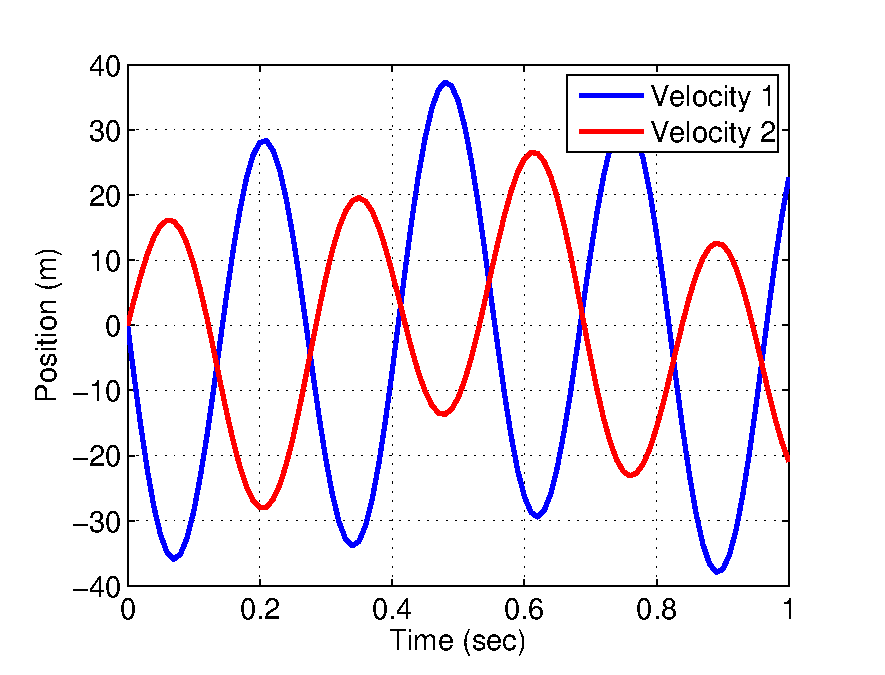
\includegraphics[height=60mm,width=90mm]{Graphics/SpringMassVelocity} \\
                         {\bf Position (m) vs Time (sec)}
                         &
                         {\bf Velocity (m/s) vs Time (sec)}
       \end{tabular}
     \end{center}
   \end{figure}

   The basic code required to plot the solution is shown below.

   \begin{framed}
     x0 = [2;0;0;0];

     k1 = 200;k2 = 200;

     m1 = 1;m2 = 1; 

     A = [0 1 0 0;(-k1-k2)/m1 0 k2/m1 0;0 0 0 1;k2/m2 0 -k2/m2 0]; 

     t = 0:0.01:1; 

     x = zeros(4,length(t)); 

     for idx = 1:length(t) 

     ~~~~x(:,idx) = expm(A.*t(idx))*x0; 

     end 

     plot(t,x) 
   \end{framed}

   This problem can also be solved using the eigenvalue
   solution. Since there are four mode shapes the solution is given by 

   \begin{equation}
     \vec{x}(t) = a_1\vec{v}_1e^{\lambda_1 t} +
     a_2\vec{v}_2e^{\lambda_2 t} + a_3\vec{v}_3e^{\lambda_3 t} +
     a_4\vec{v}_4e^{\lambda_4 t}
   \end{equation}

   The solution to obtaining the eigenvalues and eigenvectors for a
   4x4 matrix by hand is beyond the scope of this course. Thus a
   numerical solver will be used to obtain the eigenvalues and
   eigenvectors. Using the parameters previously defined our A
   matrix is
   
   \begin{equation}
     A = \begin{bmatrix} 0 & 1 & 0 & 0 \\ -400 & 0 & 200
       & 0 \\ 0 & 0 & 0 & 1 \\ 200 & 0 & -200 & 0 \end{bmatrix} 
   \end{equation}

   Using the function $[V,L] = eig(A)$ in MATLAB produces the
   following result 

   \begin{equation}
     L = \begin{bmatrix} 22.9i & 0 & 0 & 0 \\ 0 & -22.9i & 0
       & 0 \\ 0 & 0 & 8.74i & 0 \\ 0 & 0 & 0 & -8.74i \end{bmatrix} 
   \end{equation}

   where the diagonal components are the four eigenvalues. Notice that
   the eigenvalues are actually complex eigenvalues which means there
   are actually only two mode shapes and four eigenvalues. The two
   sets of mode shapes are complex conjugates of each other. The
   $eig()$ function in MATLAB also produces the eigenvectors

   \begin{equation}
     V = \begin{bmatrix} -0.04i & 0.04 & -0.06i & 0.06i \\ 0.85 & 0.85 & 0.52
       & 0.52 \\ 0.02i & -0.02i & -0.10i & 0.10 \\ -0.53 & -0.53 & 0.85 & 0.85 \end{bmatrix} 
   \end{equation}
   
   where each column of the V matrix is an eigenvector of the
   system. Note again that the real components of columns 1 and 2 are
   the same while the imaginary components are different. The same is
   true with columns 3 and 4. The $a$ coefficients are solved by using the formula $\vec{a} =
   V^{-1}\vec{x}_0$. This can also be solved by simply using a
   numerical solver.

   \begin{equation}
     \vec{a} = \begin{Bmatrix} 19.5i \\ -19.5i \\ 4.63i
       \\ -4.63i \end{Bmatrix}
   \end{equation}

   Using these coefficients, eigenvalues and eigenvectors
   it is possible to write the solution of the system. 

   \begin{equation}
     \vec{x}(t) = 19.5i\begin{Bmatrix} -0.04i \\ 0.85 \\ 0.02i \\
     -0.53 \end{Bmatrix} e^{22.9i t} -
     19.5i\begin{Bmatrix} 0.04i \\ 0.85 \\ -0.02i \\
     -0.53 \end{Bmatrix}e^{-22.9i t} + 
     4.63i\begin{Bmatrix} -0.06i \\ 0.52 \\ -0.10i \\
     0.85 \end{Bmatrix} e^{8.74i t} -
     4.63i\begin{Bmatrix} 0.06i \\ 0.52 \\ 0.10i \\
     0.85 \end{Bmatrix}e^{-8.74i t}
   \end{equation}
   
   Remember that if Euler's formula is used the two exponent's will be
   combined to produce $sines$ and $cosines$. Still, this result is
   very powerful because it tells you the two fundamental frequencies
   associated with this system. This solution can also be implemented easily
   in a numerical program such as MATLAB.

   \begin{framed}
     [V,L] = eig(A);

     a = inv(V)*x0;

     xEigen = zeros(4,length(t));

     for idx = 1:length(t)

     ~~~~~~~for n = 1:4

     ~~~~~~~~~~~~xEigen(:,idx) = xEigen(:,idx) + a(n)*V(:,n)*exp(L(n,n)*t(idx));

     ~~~~~~~end

     end

     plot(t,xEigen)
   \end{framed}

\end{enumerate}


\subsection{Example Problems}

\begin{enumerate}

\item Euler's method has a unique property in that it convertes a
  continuous differential equation such as the one below 

\begin{equation}
\ddot{y} + 2\dot{y} + 4y = 0
\end{equation}

into a discrete differential equation like the form below.

\begin{equation}
\begin{matrix}
{y}_{n+1} = {y}_n + \dot{y}_n\Delta t \\
\dot{y}_{n+1} = \dot{y}_n + (-2\dot{y}_n - 4y)\Delta t
\end{matrix}
\end{equation}

We've done this problem a
million times but what we haven't done is placed Euler's method into
the following form. 

\begin{equation}
\begin{Bmatrix}
y_{n+1} \\ \dot{y}_{n+1} \end{Bmatrix} = \begin{bmatrix} 1 & \Delta t
  \\ -4\Delta t & (1-2\Delta t) \end{bmatrix} \begin{Bmatrix} y_{n}
  \\ \dot{y}_n \end{Bmatrix}
\end{equation}

In this form it is possible to use vector algebra to compute the
solution to the differential equation. 

\begin{equation}
\vec{y}_{n+1} = A\vec{y}_n
\end{equation}

First, take your function from before spring break

\textcolor{blue}{function} myEuler(deltat)

and edit it to use the matrix form of Euler's method. Do the same
thing you did last time where you vary the timestep until the graph
does not change. However, this time compute the eigenvalues of the
matrix A. What do you notice about eigenvalues of the matrix as the
timestep gets smaller? What happens to the eigenvalues when the
timestep is too big and the graph goes unstable?

\item Simulate the multi body system derived in this chapter. Use the
  following data below.

  m1 = 2;\\
  m2 = 3;\\
  k1 = 50;\\
  k2 = 100;\\
  x1(t=0) = 5;\\
  xdot1(t=0) = 0;\\
  x2(t=0) = 10;\\
  xdot2(t=0) = 0;\\
  
  You will create the solution to the differential equation using three
  different methods. 

  \begin{enumerate}

    \item RK4

    \item z(t) = expm(A*t)*z0 - The analytical solution

    \item z(t) = V*expm(L*t)*inv(V)*z0 - Eigenvalue solution

  \end{enumerate}

  where V is the eigenvalues and L is the eigenvectors. You can use
  the eig function \\
  \ \\
  For plotting, plot all velocities (xdot1 and xdot2) for all three
  solutions on the same graph. All lines should be on top of each
  other.  \\
  \ \\
  In addition plot all positions (x1 and x2) for all three solutions
  on the same graph. Again, all lines should match. \\
  \ \\
  LIST THE EIGENVALUES OF THE A MATRIX IN YOUR REPORT. Explain what
  the eigenvalues mean in your own words. How many eigenvalues are
  there? Why are there so many? How many degrees of freedom does your
  system have? 

\end{enumerate}


\subsection{Numerical Differentiation - Chapter 23}

\begin{enumerate}

  \item {\bf Numerical Differentiation}

    Recall that the taylor series expansion for $f(x)$ is

    \begin{equation} 
      f(x_1) = f(x_0) + f'(x_0)\Delta x + f''(x_0)\Delta x^2/2! +
      ... + O(\Delta^3)
    \end{equation}

    If the equation above is truncated to first order it is possible
    to solve for $f'(x_0)$

    \begin{equation}
      f'(x_{i}) \approx \frac{f(x_{i+1})-f(x_i)}{\Delta x}
    \end{equation}

    The equation above is known as the first order approximation to
    the first derivative. There are other ways to compute the first
    derivative. The equations below are known as backward differencing
    and midpoint differencing.
    
    \begin{equation}
      f'(x_{i}) \approx \frac{f(x_{i})-f(x_{i-1})}{\Delta x}
    \end{equation}

    \begin{equation}
      f'(x_{i}) \approx \frac{f(x_{i+1})-f(x_{i-1})}{2 \Delta x}
    \end{equation}

    Note that the equations above only work for the first
    derivative. Assume however I have a function f(x) and 3 data
    points $x_0,x_1,x_2$. How would one obtain $f''(x_1)$  using
    finite differencing. First assume that $\Delta x =x_2-x_1=x_1-x_0$
    to make the math easier so $x_2-x_0=2\Delta x$. First we start by
    writing $f(x_2)$ using a 1st order expansion about $x_1$.

    \begin{equation}
      f(x_2) = f(x_1) + f'(x_1)\Delta x
    \end{equation}

    Then using that equation the first order derivative is derived as
    shown below

    \begin{equation}
      f'(x_{1}) \approx \frac{f(x_{2})-f(x_{1})}{\Delta x}
    \end{equation}

    The next step involves estimating $f(x_0)$ using $x_1$ as the
    expansion point. 

    \begin{equation}
      f(x_0) = f(x_1) - f'(x_1)\Delta x
    \end{equation}

    Note the minus sign. This equation can be used to get the backward
    differencing equations. 

    \begin{equation}
      f'(x_{1}) \approx \frac{f(x_{1})-f(x_{0})}{\Delta x}
    \end{equation}

    Using the forward and backward finite differencing equations the
    midpoint formula can be derived as shown

    \begin{equation}
      f'(x_{1}) \approx \frac{f(x_{2})-f(x_{0})}{2 \Delta x}
    \end{equation}

    Then, we estimate $f(x_2)$ using a second order expansion about
    $x_1$.

    \begin{equation}
      f(x_2) = f(x_1) + f'(x_1)\Delta x + \frac{f''(x_1)}{2!}\Delta
      x^2
    \end{equation}

    Using the equation above, substituting in the midpoint
    differencing formula and solving for $f''(x_1)$ yields the
    equation below.

    \begin{equation}
      f''(x_{1}) \approx \frac{f(x_{2}) -2 f(x_{1}) +
        f(x_0)}{\Delta x^2}
    \end{equation}
      

  \item {\bf Higher Order Differentiation}

    The equations above were simply first order approximations to the
    first and second derivatives. It is possible to truncate the
    taylor series to second order and solve for the first
    derivative. Thus the second order approximation to the first
    derivative is

    \begin{equation}
      f'(x_i) = \frac{-f(x_{i+2})+4f(x_{i+1})-3f(x_i)}{2\Delta x}
    \end{equation}

    %% In order to obtain higher and higher order derivatives the taylor
    %% series expansion must be truncated at higher and higher terms. It
    %% is possible however to use Romberg Integration to obtain higher
    %% derivatives. For example if $D_{1,1}$ is a first order
    %% approximation to the first derivative using $N_1$ intervals and
    %% $D_{2,1}$ is a first order approximation to the first derivative
    %% using $N_2$ then $D_{1,2}$ is simply

    %% \begin{equation}
    %%   D_{1,2} = \frac{4}{3} D_{2,1} - \frac{1}{3}D_{1,1}
    %% \end{equation}

    Note that these methods show a perfect example of truncation error
    and roundoff error. Assume for the moment that we would like to
    differentiate $(x^3)$ at $x=2$. It is easy to see that the
    analytical solution is just 12. However if we use the first and
    second order approximations and plot the error as a function of
    our increment we get the following graph.

    \begin{figure}[H]
      \begin{center}
        \includegraphics[height=0.55\textwidth,width=0.7\textwidth]{Graphics/Round_Off_Truncation.pdf}
      \end{center}
    \end{figure}
    
    Notice here that we can directly see that increasing our timestep
    reduces our round-off error. We can reduce our truncation error by
    using a higher and higher order method however we will always hit
    our limit of precision.

  \item {\bf Bicycle Sensor}

    Let's say I'd like to know my speed and distance while riding a
    bike. The easiest thing to do would be to install a sensor on the
    fork and the tire. When the sensor on the fork is in sync the main
    controller saves the time this happens in the form

    \begin{equation}
      T_{sync} = [T_1 \hdots T_N] 
    \end{equation}

    The task is then to extract velocity and distance from this
    equation. The first order derivative of velocity can be written in
    the form
    
    \beq
    V_i = \frac{x_{i+1} - x_i}{T_{i+1}-T_i} = \frac{\Delta x}{T_{i+1}-T_i}
    \eeq

    The question is what is $\Delta x$? $\Delta x$ is the distance the
    wheel travels during one click which is simply the circumference
    of the tire so we arrive at the equation below.

    \beq
    V_i = \frac{2\pi r}{T_{i+1}-T_i}
    \eeq

    To obtain the distance travelled we can apply the standard
    Reimmann Sum to the velocity equation above we obtain

    \beq
    x_N = x_0 + \sum\limits_{i=0}^N V_i \Delta T_i = \sum\limits_{i=0}^N
    \frac{2\pi r}{T_{i+1}-T_i}\Delta T_i = \sum\limits_{i=0}^N 2\pi r
    \eeq
  
    where $N$ is the number of times the sensor passes the main
    fork. Notice now that the sum does not depend on $i$ thus the
    distance is simply

    \beq
    x_N = x_0 + N2\pi r
    \eeq

    Which means we now have a method to determine velocity and
    distance traveled. As an example, try and verify the velocity and
    distance travelled using the timestamps below. Assume you're
    riding 14 inch tires.

    \beq
    \begin{matrix}
    T = [0,1.1320,4.1921,6.4561,8.3252,10.0598]~sec\\
    V = [6.4758,2.3955,3.2377,3.9219,4.2260]~ft/s\\
    X = [0,7.3304,14.6608,21.9911,29.3215,36.6519]~ft
    \end{matrix}
    \eeq

    \item {\bf Problems with Derivatives}
      
      Let's say I have a GPS sensor on an airplane traveling 800
      ft/s. This GPS sensor gives me two measurements. First the
      position in feet (Not really but we can just assume this for
      classroom example purposes).

      \beq
      X = [x_1 \hdots x_N] 
      \eeq

      The GPS is also timestamped and thus returns the time coordinate

      \beq
      T = [t_1 \hdots t_N]
      \eeq

      This seems like a simple problem. Just differentiate it and get

      \beq
      V_i = \frac{x_{i+1}-x_i}{t_{i+1}-t_{i}}
      \eeq

      The problem is real sensors have noise. So I can't actually know
      what $X$ is really and instead I obtain $\hat{X}$ which is my
      sampled measurement or output from the GPS sensor. Let's assume
      that my GPS is accurate to 25 ft. I can model this as:

      \beq\label{e:sampledX}
      \hat{X} = X + N(0,25)
      \eeq
      
      where $N(0,25)$ is a random uniform number with a mean of zero
      and a standard deviation of 25 ft. If we return to our numerical
      derivative we obtain

      \beq
      \hat{V}_i = \frac{\hat{x}_{i+1}-\hat{x}_i}{t_{i+1}-t_{i}}
      \eeq

      Ok so how bad is this? Let's compute the error between $V_i$ and
      $\hat{V}_i$.
      
      \beq
      V_i - \hat{V}_i =
      \frac{\hat{x}_{i+1}-\hat{x}_i}{t_{i+1}-t_{i}} -
      \frac{{x}_{i+1}-{x}_i}{t_{i+1}-t_{i}} = \frac{\hat{x}_{i+1}-\hat{x}_i -
        {x}_{i+1} + {x}_i}{t_{i+1}-t_{i}}
      \eeq

      If we substitute in equation \ref{e:sampledX} we obtain

      \beq
      V_i - \hat{V}_i =
      \frac{{x}_{i+1}+N_{i+1}-{x}_i-N_{i}-{x}_{i+1} +
        {x}_i}{t_{i+1}-t_{i}} = \frac{N_{i+1}-N_{i}}{t_{i+1}-t_{i}}
      \eeq

      Ok so let's substitute real number in here and obtain the
      maximum error remembering that GPS updates at 4 Hz = 0.25 sec

      \beq
      |V_i - \hat{V}_i|_{max} = \frac{|N_{i+1}-N_{i}|_{max}}{0.25 sec}
      \eeq

      So what is $|N_{i+1}-N_{i}|_{max}$. Well, the maximum of $N_i$
      is 25 ft which means that max of
      $|N_{i+1}-N_{i}|_{max}=25~ft$ which leads to 

      \beq
      |V_i - \hat{V}_i|_{max} = \frac{25~ft}{0.25~sec} = 100 ft/s
      \eeq

      Remember, we were flying at 800 ft/s and we could be off by as
      much as 100 ft/s! That's over 12.5\%. Notice however that, the
      velocity error is independent of flight speed so what would
      happen if we were riding a bike and our speed was say 10 ft/s?
      This would mean our velocity measurement was off by an order of
      magnitude. 
      
    \item {\bf Filters}

      We've shown in the previous derivation that derivatives
      introduce alot of noise in the measurement. So what do we do?
      The easiest thing to implement is what's called a complimentary
      filter. It is a simplification of the Kalman Filter created by
      Rudolf Kalman in 1960. The basic derivation goes like this,
      assume the input signal is $\hat{y}$ and the output filtered
      signal is $\tilde{y}$. This is the setup for all types of
      filters. In this setup we use the equation below

      \beq
      \tilde{y}_{i+1} = \sigma \hat{y}_{i+1} + (1-\sigma)\tilde{y}_{i}
      \eeq

      This may seem simple and it is but it's pretty
      powerful. Remember that the system is iterative so 

      \beq
      \begin{matrix}
        \tilde{y}_1 = \sigma \hat{y}_{1} + (1-\sigma)\tilde{y}_{0}\\
        \tilde{y}_2 = \sigma \hat{y}_{2} + (1-\sigma)\tilde{y}_{1}\\
        \tilde{y}_3 = \sigma \hat{y}_{3} + (1-\sigma)\tilde{y}_{2}\\
        \vdots\\
        \tilde{y}_N = \sigma \hat{y}_{N} + (1-\sigma)\tilde{y}_{N-1}
      \end{matrix}
      \eeq
      
      Notice that in this equation $\tilde{y}_0$ cannot be defined
      thus a separate equation is used for the initial condition. 

      \beq
      \tilde{y}_0 = \hat{y}_0
      \eeq

      With this setup we can now show some examples. Let's
      assume that $\sigma = 1$. In this scenario $\tilde{y}_i = \hat{y}_i$
      which means the signal is not filtered. If $\sigma = 0$,
      $\tilde{y}_{i+1} = \tilde{y}_i$. Since $\tilde{y}_0=\hat{y}_0$
      it means that that $\tilde{y}_i=\hat{y}_0$. However, if we
      return to the example where we have our GPS sensor on board and
      set $\sigma=0.03$ we obtain the following result. The other
      thing we can do of course is simply average the result. 

      \begin{figure}[H]
        \begin{center}
          \includegraphics[height=0.5\textwidth,width=0.7\textwidth]{Graphics/Airplane_Sensor_Constant}
        \end{center}
      \end{figure}

      Now averaging the result would be easy when the speed is
      constant but airplanes rarely fly at constant speeds. What if
      the speed was more sinusoidal reflecting the changes in flight
      speed from atmospheric winds.

      \begin{figure}[H]
        \begin{center}
          \includegraphics[height=0.5\textwidth,width=0.7\textwidth]{Graphics/Airplane_Sensor_Variable}
        \end{center}
      \end{figure}

      In the graph you can see that averaging the result does not
      simply capture the changes in the velocity of the airplane hence
      why the complimentary filter is so useful.
    
\end{enumerate}




\subsection{Driving Lab Experiment}

Your task is to team with two other lab partners and go for a ride
around the town or get some coffee or just run an errand. Here are the rules.

\begin{enumerate}

\item The driver is responsible for one thing and that is driving. Do
  not take your eyes off the road or text while driving. You must be
  safe at all times and get all of your passengers to and from your
  destination safely. For this assignment the driver must own a
  vehicle with a functioning odometer and speedometer.  I would
  recommend resetting your trip meter. If your car does not have a
  trip meter you must write down the initial mileage of your vehicle
  before you depart. 

\item Passenger number 1. Your task is to read off the drivers speed
  every 10 seconds on the departure leg and every 30 seconds on the
  return leg. I would bring a pencil and paper or your computer with
  excel open and write down the time in intervals of 10 seconds on the
  departure leg and 30 seconds for the return leg. While the car is
  driving you can then write down the speed by looking at the
  speedometer and writing the speed in mph. I would recommend
  converting mph to miles/second so that your units will match up. 

\item Passenger number 2 is responsible for measuring the distance
  traveled in units of 0.1 miles using the odometer. I would recommend
  synchronizing watches with passenger number 1 and passenger number 2
  so that your time vectors line up. Your table should have time in
  one column and position in increments of 0.1 miles in another
  column.

\end{enumerate}

Once all of this data is compiled you need to generate the following plots.

\begin{enumerate}

\item Velocity versus time

\item Position versus time

\item Use first order differentiation and compute velocity versus time
  using part b. Plot this alongside part a and compare your
  results. For the down leg and the return leg. Which is more
  accurate? 

\item Use the trapezoidal rule to compute position versus time using
  part a and plot it alongside part b. Compare your results with the
  down leg and the return leg. Which is more accurate? 

NOTE ALL THREE OF YOU MUST COMPLETE THE ASSIGNMENT. YOU MAY
TAKE DATA AND HAVE FUN TOGETHER BUT EVERYONE MUST STILL COMPLETE THE
LAB.  

\end{enumerate}



\subsection{Output Error Method}

\begin{enumerate}

\item{\bf Output Error Method}

Newton-Raphson works great when you have one output and one variable
trying to be determined using a direct correlation. For example, let's
assume I place an aircraft in a wind tunnel and I vary the wind
tunnel speed while changing the angle of attack such that Lift is
equal to Weight. I have a load sensor on board that measures Drag such
that I can plot Drag as a function of velocity. Explicitly I
would have $D = f(V)$. Using this function, I could compute the
drag coefficient using the simple formula. 

\begin{equation}
D_i = \frac{1}2\rho V_i^2 S C_{Di}
\end{equation}

The subscript $i$ is in the formula above because I have multiple
velocity and drag readings. The method defined above is typical for
operators in a wind tunnel. Using the drag as a function of velocity
you can obtain the drag coefficient as a function of velocity. Using
the drag coefficient I could also find the speed for minimum drag
using the standard Newton-Raphson technique.

\begin{equation}
V_{i+1} = V_i - \frac{f'(V_i)}{f''(V_i)}
\end{equation}

The issue is that you can only obtain the drag coefficient and nothing
else using a wind tunnel. The reason for this is that the aircraft in
the wind tunnel is static and you can only measure certain
coefficients at a time. For example, you could measure lift as well
and estimate the lift coefficient but let's assume you want damping
coefficients. To do this you need to use the output error method.
Let's assume instead that I actually fly the airplane and instead of
measuring velocity and drag, I measure time and distance. Thus I have
$x=f(t)$. Here, I want to find the drag coefficient but notice that I
do not have have the drag anymore. Thus, I can't use Newton-Raphson
technique explicitly but with some massaging I can cast the problem
into a better form. First if we assume the aircraft flies in one
dimension I can write the equations of motion of the aircraft to be

\begin{equation}
\ddot{\tilde{x}} = -\frac{1}{2m}\rho \dot{\tilde{x}}^2 S \tilde{C}_D
\end{equation}

Notice, here that suddenly our drag coefficient pops up. What we can
do then is create an initial guess for our drag coefficient, then use
a numerical integration technique to get an estimate for x. Using this
we can actually create an error estimate as a function of time.

\begin{equation}
\tilde{E}(t) = x(t) - \tilde{x}(t)
\end{equation}

from here we can create an average error square estimate such that

\begin{equation}
J = \frac{1}N\sum\limits_{i=1}^N |\tilde{E}(t_i)|^2
\end{equation}

Let's recap all we've done. We now have an error estimate $J$
which is a function of our drag estimate $\tilde{C}_D$. Formally we have
$J=f(\tilde{C}_D)$. Typically J is called a cost function. If we choose
$\tilde{C}_D$ that is the same as the actual value of $C_D$ then we
would have a cost of 0. This is our ideal situation. It might be
tempting to simply use a root finding method but in fact we actually
want to minimize J. Often times we cannot reach a zero cost given
modeling errors, truncation errors, sensor errors, and round off
errors. However we can still estimate $C_D$ using the recursive
algorithm as defined in the Newton-Raphson method.

\begin{equation}
\tilde{C}_{D,i+1} = \tilde{C}_{D,i} - \frac{J'(\tilde{C}_{D,i})}{J''(\tilde{C}_{D,i})}
\end{equation}

Note that the first and second derivatives of the cost function must
be computed numerically. This is a very involved process with multiple
parts from this course. This entire method is called the Output Error
Method.

\item {\bf Example}

This assignment will involve the students splitting into groups to
write codes that perform the Output Error Method. The Output Error
Method is a way to solve for unknowns where there is no analytical
solution available. For example, let us examine the parachute in free
fall. The equations of motion are

\begin{equation}\nonumber
\ddot{z} = -g + \frac{1}{2m}\rho\dot{z}^2SC_D
\end{equation}

This equation can be simulated on a modest computer assuming all
parameters are known. Assume for the moment that the data $z(t)$ has
been given in a table format. Then assume that the initial conditions
and all parameters except $C_D$ are given:
\ \\

\begin{center}\begin{tabular}{l l l l l l}
$z_0$ = 100 m & $\dot{z}_0$ = 0 m/s & g = 9.81 $m/s^2$ & $\rho$ =
    1.225 $kg/m^3$ & S = 1 $m^2$ & m = 10 kg
\end{tabular}\end{center}

The question then is how to solve for the drag coefficient $C_D$. To
do this the output error method is used. 

\begin{enumerate}

\item The method starts with an initial guess $\tilde{C_D}$.

\item This initial guess can be used to obtain $\tilde{z}$.

\item The total error between the computed value $\tilde{z}$ and the
  measured data from the input file $z$ can be computed using the
  equation below.

  \begin{equation}
    E = \frac{1}N\sum\limits_{i=1}^N (z(t_i)-\tilde{z}(t_i))^2
  \end{equation}
  
  The goal then naturally is to perform an optimization technique and
  compute $\tilde{C_D}$ such that the error drops to zero or at least
  a minimum.

 \item To minimize this problem the Newton-Raphson technique is used
   such that

   \begin{equation}
     \tilde{C}_{D,i+1} = \tilde{C}_{D,i} - \frac{E'(\tilde{C}_{D,i})}{E''(\tilde{C}_{D,i})}
   \end{equation}

   Obviously the first and second derivatives will need to be computed numerically.

\end{enumerate}

To solve this problem the students will break into groups of 6 or 7. Each
member of the group will have to complete one of the codes
below. Built in MATLAB functions are allowed unless noted specifically
in the text. Note that the group may opt to work as a team
on certain sections of the code.

\begin{enumerate}

\item function [t,z] = readdata(filename), this function will use the
  dlmread() command to read the text file of data provided and return
  the t vector, z vector and the timestep used to generate the data.

\item function ploteverything(t,z,ztilde), this function will take a
  vector t, z and ztilde and plot everything in a nice pretty graph

\item function zdot = Derivs(t,z,CDtilde), this function will compute the
  derivative of z for a given value of CDtilde. Remember that z will
  be a vector containing $z$ and $\dot{z}$ thus zdot will be a
  vector containing $\dot{z}$ and $\ddot{z}$ 

\item function [ttilde,ztilde] = RK4(CDtilde), this function will take
  a value of the drag coefficient and use the RK4 method to compute
  the height of the parachute as a function of time. Note that you
  need to make sure you use the same timestep as the one used in the
  data set provided. You may not use the ode45() function.

\item function E = compute\_error(CDtilde,z), this function will
  compute the total error between the estimated height ztilde and the
  actual height z.

\item function fprime = Eprime(CDtilde,z), this function will compute
  the first derivative of the error function at the value of
  CDtilde. Remember that you will have to choose the value of
  $\Delta$. 

\item function fdblprime = Edoubleprime(CDtilde,z), this function will
  compute the second derivative of the error function at the value of
  CDtilde. Again you must choose $\Delta$

\item function main(), this function will perform the optimization. I
  have written this part of the code for you.

\begin{framed}

function main()

filename = 'drc\_data.txt';

[t,z] = readdata(filename);

CDtilde = 0.1;

Ei = compute\_error(CDtilde,z);

while abs(Ei) $>$ 1e-2

~~~~~~CDtilde = CDtilde - Eprime(CDtilde,z)/Edoubleprime(CDtilde,z);

~~~~~~Ei = compute\_error(CDtilde,z);

end

[ttilde,ztilde] = RK4(CDtilde);

ploteverything(t,z,ztilde);

\end{framed}

\end{enumerate}

The winning team must solve for $C_D$ and email the instructor a graph
showing z and ztilde on top of each other. The first team to correctly
email the instructor with the value of $C_D$ and the correct graph
will get a prize. Ready go!

\end{enumerate}




\section{FINITE DIFFERENCE/ELEMENTS METHOD}

\begin{enumerate}

  \item {\bf Boundary-Value Problems}\label{s:heat1D}

    The heat equation on the other hand is a boundary value problem. Here we
    represent the pipe without time such that $T = f(x)$ instead of
    time. 

    \begin{equation} 
      \frac{d^2 T}{d x^2} - h'(T-T_a) = 0
    \end{equation}
    
    Thus the difference between boundary value problems and initial
    condition problems is really the independent variable. To solve
    this we set $T = Ce^{sx}+T_a$. We substitute this equation into 
    the equation above and obtain the characteristic equation and
    solve for s = $\pm\sqrt{h'}$. This yields the analytical solution
    $T(x) = A e^{\sqrt{h'}x} + B e^{-\sqrt{h'}x} + T_a$. Again the boundary
    conditions can be used to solve for A and B. For example, $T(x=0)
    = 40$ and $T(x=L) = 200$. Note that solving for A and B yields a
    system of equations. The solution to A and B has been left for the
    reader. 

    Now, in order to solve this equation numerically you must replace
    all derivatives with finite difference approximations. Below is a
    center first order approximation of the second derivative.

    \begin{equation}
      \frac{T_{i+1} - 2T_i + T_{i-1}}{\Delta x^2} - h'(T_i-T_a) = 0
    \end{equation}

    or

    \begin{equation}
      -T_{i-1} + (2+h'\Delta x^2)T_i - T_{i+1} = h'\Delta x^2 T_a
    \end{equation}

    If the rod is discretized into 6 beads ($\Delta x = 2$ and L = 10
    m) such that $T(0) = T_0 = 40$ and $T(L) = T_5 = 200$, letting
    h'=0.01 and $T_a = 20$ yields a system of equations

    \begin{equation}
      \begin{bmatrix} 2.04 & -1 & 0 & 0 \\ -1 & 2.04 & -1 & 0 \\ 0 &
        -1 & 2.04 & -1 \\ 0 & 0 & -1 &
        2.04\end{bmatrix} \begin{Bmatrix} T_1 \\ T_2 \\ T_3
          \\ T_4 \end{Bmatrix} = \begin{Bmatrix} 40.8 \\ 0.8 \\ 0.8
          \\ 200.8 \end{Bmatrix}
    \end{equation}

    which can be solved with any numerical solver. In this case $T = [
      65.970,93.778,124.538,159.480]$. Note, this can also
    be done using an iterative method. If the candidate equation is
    written such that
    
    \begin{equation}
      T_{i} = \frac{T_{i-1} + h'\Delta x^2 T_a + T_{i+1}}{2+h'\Delta x^2}
    \end{equation}

    The problem above evolves into a Simple Fixed Point Iteration
    Problem where the output is computed for every location $i$ along
    the rod and the solution is used to compute the next solution. The
    code required to implement the Simple Fixed Point Iteration
    technique is shown below.

    \begin{framed}
      x = 0:2:10;

      Tguess = 0*x;

      Tguess(1) = 20;

      Tguess(end) = 200;

      Ta = 20;

      hprime = 0.01;

      for iter = 1:100

      ~~~~~~for idx = 2:length(Tguess)-1

      ~~~~~~~~~~~~Tguess(idx) = (Tguess(idx-1) + hprime*delx{\textrm{\^}2}*Ta + Tguess(idx+1))/(2+hprime*delx{\textrm{\^}2});

      ~~~~~~end

      end
    \end{framed}

    The benefit of this code over solving the system using
    $A\vec{x}=B$ is that the number of beads can be arbitrarily
    increased without any change to the code. The solution to the code
    above can be plotted alongside the analytical solution and is
    shown in the equation below. Note that the solution below has 11
    beads rather than 6 beads. 

    \begin{figure}[H]
     \begin{center}
       \includegraphics[height=0.4\textwidth,width=0.5\textwidth]{Graphics/Heat_Equation}
     \end{center}
   \end{figure}

\end{enumerate}


\subsection{Partial Differential Equations - Chapter 29}

\begin{enumerate}

  \item {\bf Overview of PDEs}

    All equations we've dealt with thus far involves functions of one
    dimension $f(t)$ (initial value problems) or $f(x)$ (boundary value
    problems). In engineering, problems are rarely one-dimensional and
    usually involve multiple independent variables $f(x,y,z,t)$
    (spatially and temporally varying wind field for example). Most
    systems encountered in engineering are second order and can be
    expressed using the equation below.

    \begin{equation} 
      A \frac{\partial^2 u}{\partial x^2} + B \frac{\partial^2
        u}{\partial x \partial y} + C \frac{\partial^2 u}{\partial y^2}
      + D = 0
    \end{equation}
    
    If $B^2-4AC < 0$ the equation is elliptic. If $B^2-4AC = 0$ the
    equation is parabolic and if $B^2-4AC > 0$ the equation is
    hyperbolic. 

  \item {\bf Elliptic Equations}

    The 2-D heat transfer governing equation is

    \begin{equation}
      k_x \frac{\partial^2 T}{\partial x^2} + k_y \frac{\partial^2
        T}{\partial y^2} + Q = \frac{2h}{t} (T-T_\infty)
    \end{equation}
    
    where $k$ is the thermal conductivity, $T$ is the temperature, $Q$
    is the heat source, $h$ is the convection coefficient and $t$ is
    the plate thickness. If the plate is insulated on its lateral
    surfaces(top and bottom), $k_x=k_y=k$ and $Q=0$, the governing equation becomes 

    \begin{equation}
      \frac{\partial^2 T}{\partial x^2} + \frac{\partial^2
        T}{\partial y^2} = 0
    \end{equation}
    
    In the general form this means that A = 1, B = 0, C = 1 and C = 0
    thus $B^2-4AC = -4 < 0$ which means the equation is elliptic. In
    order to solve this equation the system is discretized into a set
    of grid points. Then the partial derivatives can be approximated
    using central difference formulas.

    \begin{equation}
      \frac{T_{i+1,j} - 2T_{i,j} + T_{i-1,j}}{\Delta x^2} +
      \frac{T_{i,j+1} - 2T_{i,j} + T_{i,j-1}}{\Delta y^2} = 0
    \end{equation}

    If $\Delta x = \Delta y$ the equation reduces to 
    
    \begin{equation}\label{e:heat_equation2d}
      T_{i+1,j} + T_{i-1,j} + T_{i,j+1} - 4T_{i,j} + T_{i,j-1} = 0
    \end{equation}

    Assume you start with grid point $i=1$ and $j=1$. The equation is
    then

    \begin{equation}
      T_{2,1} + T_{0,1} + T_{1,2} - 4T_{1,1} + T_{1,0} = 0
    \end{equation}
    
    If boundary conditions are used such that $T_{0,j} = 75^o$,
    $T_{i,0} = 0^o$, $T_{4,j} = 50^o$ and $T_{i,4} = 100^o$ (assume a
    3x3 grid) the equation above reduces to

    \begin{equation}\label{e:heat_example}
      \begin{matrix}
      T_{2,1} + 75 + T_{1,2} - 4T_{1,1} + 0 = 0 \\
      T_{2,1} + T_{1,2} - 4T_{1,1}  = -75
      \end{matrix}
    \end{equation}

    Note that when boundary conditions are given this is known as
    Dirichlet boundary conditions, that is the temperature is held
    constant. If instead the sides are insulated it means the heat
    flux ($\partial T/\partial x$) is zero. Thus the derivative is
    given instead of the value. This is known as a Neumann condition. 

    Repeating equation \ref{e:heat_example} for all 9 grid points yields a system of
    the form $A\vec{x} = b$ where A is a 9x9 matrix. This can then be
    solved by any numerical solver just like the single dimension
    boundary value problem. 

    The solution is shown in the matrix below

    \begin{equation}
      T(x,y) = \begin{bmatrix} 43.0000   & 33.3000 &  33.8900 \\
        63.2100 &  56.1100 &  52.3400 \\
        78.5900 &  76.0600 &  69.7100 \\
      \end{bmatrix}
    \end{equation}
    
    This can be plotted in MATLAB using the function below

    \begin{framed}
      x = 1:3;
      
      y = 1:3;
      
      [xx,yy] = meshgrid(x,y);

      Tsolution = [43 33.3 33.89;63.21 56.11 52.34;78.59 76.06 69.71];

      mesh(xx,yy,Tsolution)

    \end{framed}

    Notice that MATLAB matrices are top to bottom so make sure you
    enter the solution in correctly otherwise you will get incorrect results.

    \begin{figure}[H]
     \begin{center}
       \includegraphics[height=0.4\textwidth,width=0.5\textwidth]{Graphics/Heat_Equation2D}
     \end{center}
   \end{figure}

\item {\bf Gauss-Seidel Method}

    Just as in the single dimensional heat equation the process of
    creating the matrices above is very tedious when performing this
    by hand. Thus it is beneficial to create a routine that can
    iterate until convergence. Taking equation \ref{e:heat_equation2d}
    and rearranging for $T_{i,j}$ yields 

    \begin{equation}
      T_{i,j} = (T_{i+1,j} + T_{i-1,j} + T_{i,j+1} + T_{i,j-1})/4
    \end{equation}
    
    This again can be easily implemented into a numerical solver just
    as before. The code has been left out so that the reader may
    attempt to create this code as an exercise however the error
    between the iterative solution and the solution from above even
    after 10 iterations is on the order of $10^-3$ as shown by the
    mesh plot of the error below. Of course this is specific to the
    initial guess but the iterative method is still robust to changes
    in grid size. This is known as the Gauss-Seidel Method.
    
    \begin{figure}[H]
     \begin{center}
       \includegraphics[height=0.4\textwidth,width=0.5\textwidth]{Graphics/Heat_Equation2D_Error}
     \end{center}
   \end{figure}    

  \item {\bf Derivative Boundary Conditions}

    If derivative boundary conditions are introduced we no longer have
    the value of T at the boundary. Instead we have the value of the
    derivative. In order to incorporate the derivative boundary the
    central difference equation is written for the boundary point such
    that

    \beq
    T_{1,j} + T_{-1,j} + T_{0,j+1} + T_{0,j-1} - 4 T_{0,j} = 0
    \eeq

    Notice that the variable $T_{-1,j}$ has been introduced which is
    outside the boundary. However this variable can be used to
    substitute the derivative into the finite difference equations.

    \beq
    \frac{\partial T_{0,j}}{\partial x} =
    \frac{T_{1,j}-T_{-1,j}}{2\Delta x}
    \eeq
    
    The equation above can be solved for $T_{-1,j}$ and substituted
    into the $0,j$ equation to yield

    \beq
    2T_{1,j} -2\Delta x \frac{\partial T_{0,j}}{\partial x} + T_{0,j+1} + T_{0,j-1} - 4 T_{0,j} = 0
    \eeq

    The equation above can be used for all nodes with a derivative
    boundary condition to solve for the heat flux in a plate.

    \item {\bf Vibrating String}

    Another elliptic equation is the vibrating string which can be
    solved in a similar fashion.

    \begin{equation}
      T \frac{\partial^2 v}{\partial x^2} - m \frac{\partial^2
        v}{\partial t^2} = 0
    \end{equation}

    In the equation above, T is the tension in the string and m is the mass per unit
    length of the rod. $v(x,t)$ is the amount of deflection in the
    string as a function of space and time. Notice that in this
    equation the time derivative is second order. Thus Euler's method
    is not accurate enough to compute the time derivative and a higher
    order method such as a Runge-Kutta-4 scheme must be used in order
    to converge to the solution.

  \item {\bf Parabolic Equations}

    An example parabolic equation is again a heat equation however
    here the equation is a function of x and time. The equation is
    given below

    \begin{equation}\label{e:parabolic}
      k\frac{\partial^2 T}{\partial x^2} = \frac{\partial T}{\partial t}
    \end{equation}

    Just as before the spatial derivative is approximated using
    central finite differencing however a superscript has been added
    to denote the time variable. That is $T_{1}^3$ is the value of
    temperature at the first node at time t = 3.

    \begin{equation}\label{e:spaceheat}
      \frac{T_{i+1}^l - 2T_{i}^l + T_{i-1}^l}{\Delta x^2} =
      \frac{\partial^2 T}{\partial x^2}
    \end{equation}

    Similarly Euler's Method can be used to approximate the time
    derivative of T.

    \begin{equation}\label{e:timeheat}
      \frac{\partial T}{\partial t} = \frac{T^{l+1}-T^l}{\Delta t}
    \end{equation}

    If equations \ref{e:timeheat} and \ref{e:spaceheat} are
    substituted in equation \ref{e:parabolic} and rearranged for
    $T_i^{l+1}$ the Finite Difference Method equation becomes    

    \begin{equation}
      T_i^{l+1} = T_i^l + \lambda (T_{i+1}^l - 2T_i^l + T_{i-1}^l)
    \end{equation}

    where $\lambda = \frac{k\Delta t}{\Delta x^2}$. Note, just like
    Euler's method, there are limits on stability for this method. In
    Carnahan et al. 1969 it was proved that the system is stable if
    $\Delta t \leq \frac{\Delta x^2}{2 k}$. The iterative method above
    thus combines the time dependent and spatially dependent portion
    of the rod. Thus, let us return to the simple static case we saw
    in section \ref{s:heat1D} where the rod is discretized into 6
    beads ($\Delta x = 2 m$ and L = 10 m) such that $T(0) = T_0 = 40$
    and $T(L) = T_5 = 200$. However, in this case let's assume that
    the rod has no heat at all except at the end points
     such that T = [200 0
     0 0 0 200]. The iterative procedure above is used to
    propogate the system forward to see how the heat in the rod
    evolves over time where $k' = 0.49 cal/(s-cm-^oC)$. Again the code
    has been removed and left for an exercise to the reader. The
    temperature distribution as a function of time is shown in the
    figure below.

    \begin{figure}[H]
      \begin{center}
       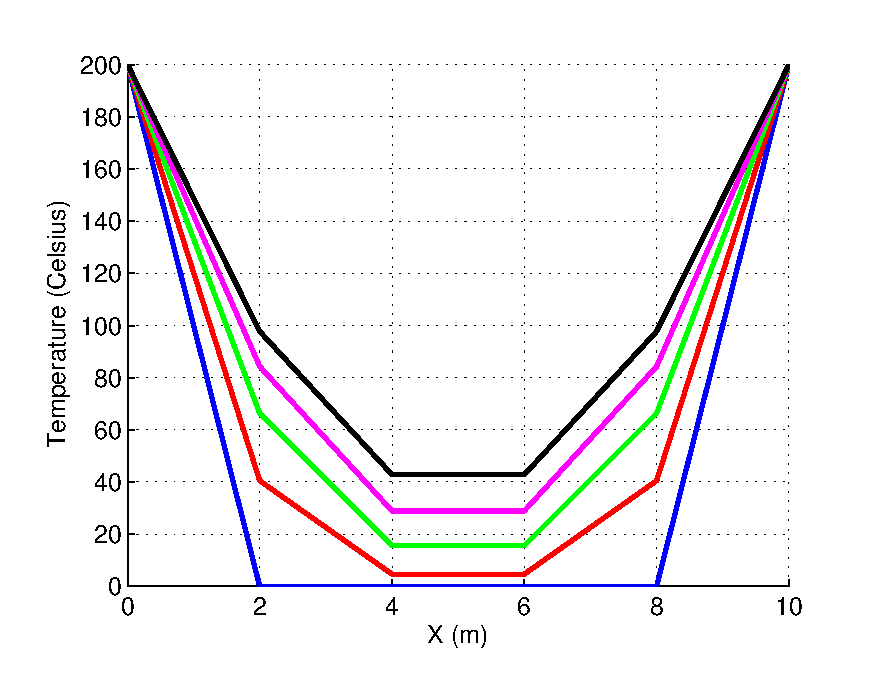
\includegraphics[height=0.4\textwidth,width=0.5\textwidth]{Graphics/Heat_Rod_Time}
      \end{center}
    \end{figure}

    This can also be visualized in three dimensions where a mesh plot
    is created. Here the x axis is the length of the rod, the y axis
    is the time variable and the z axis is the temperature along the
    rod. It is clear that the temperature in the rod is slowly heating
    up to $200^o C$.

    \begin{figure}[H]
      \begin{center}
        \includegraphics[height=0.4\textwidth,width=0.5\textwidth]{Graphics/Heat_Time_Mesh}
      \end{center}
    \end{figure}

  \item {\bf Crank-Nicolson Method}

    The Crank-Nicolson method is an implicit method rather than an
    explicit method. That is, rather than computing the next time step
    forward one at a time for each spatial coordinate, each timestep
    is computed simultaneously for the entire rod. The equations are
    obviously more complex however, it does not have the stability
    problem that the explicit method has because the spatial and time
    derivatives are second order accurate. First, the time derivative
    is approximated at the midpoint of time using the equation below.

    \beq
    \frac{\partial T}{\partial t} = \frac{T_i^{l+1}-T_i^l}{\Delta t}
    \eeq

    The spatial derivative is then approximated as an average of the
    forward point $l+1$ and the current time point $l$.

    \beq
     \frac{\partial^2 T}{\partial x^2} =
     \frac{1}{2}\left[\frac{T_{i+1}^l - 2T_{i}^l + T_{i-1}^l}{\Delta
         x^2} + \frac{T_{i+1}^{l+1} - 2T_{i}^{l+1} + T_{i-1}^{l+1}}{\Delta
         x^2} \right]
    \eeq

    Substituting these two equations into equation \ref{e:parabolic}
    results in

    \beq
    -\lambda T_{i-1}^{l+1} +2(1+\lambda) T_{i}^{l+1} - \lambda
    T_{i+1}^{l+1} = \lambda T_{i-1}^l + 2(1- \lambda)T_{i}^l + \lambda T_{i+1}^l
    \eeq

    where $\lambda = \frac{k\Delta t}{\Delta x^2}$. For the first
    point above $i=1$ the equation becomes

    \beq
    2(1+\lambda) T_{1}^{l+1} - \lambda
    T_{2}^{l+1} = \lambda T_{0}^l + \lambda T_{0}^{l+1} + 2(1- \lambda)T_{1}^l + \lambda T_{2}^l
    \eeq
    
    for the last point $i=m$, the equation becomes

    \beq
    -\lambda T_{m-1}^{l+1} +2(1+\lambda) T_{m}^{l+1}  = \lambda
    T_{m+1}^{l+1} + \lambda T_{m-1}^l + 2(1- \lambda)T_{m}^l + \lambda T_{m+1}^l
    \eeq
    
    where $T_0$ and $T_{m+1}$ are boundary conditions. These equations
    can be stacked in matrix form to yield the following equations.

    \beq
    \begin{bmatrix} 2(1+\lambda) & -\lambda & \hdots & 0 & 0 & 0 &
      \hdots & 0 & 0 \\ 0 & 0 & \hdots & -\lambda & 2(1+\lambda) &
      -\lambda & \hdots & 0 & 0 \\ 0 & 0 & \hdots & 0 & 0 & 0 &
      \hdots & -\lambda & 2(1+\lambda) \end{bmatrix} \begin{Bmatrix} T_1^{l+1}
      \\ T_2^{l+1} \\ \vdots \\ T_{i-1}^{l+1} \\ T_i^{l+1}
      \\ T_{i+1}^{l+1} \\ \vdots \\ T_{m-1}^{l+1}
      \\ T_m^{l+1} \end{Bmatrix} = \vec{b}
    \eeq

    where $\vec{b}$ is

    \beq
    \vec{b} = 
    \begin{Bmatrix} \lambda T_0^l +
      \lambda T_0^{l+1} + 2(1-\lambda) T_1^l + \lambda T_2^l \\ \vdots \\
      \lambda T_{i-1}^l + 2(1-\lambda) T_i^l + \lambda T_{i+1}^l
      \\ \vdots \\ \lambda T_{m-1}^l + \lambda T_{m+1}^{l+1} + 2(1-\lambda) T_m^l + \lambda
      T_{m+1}^l \end{Bmatrix}
    \eeq

    The assumption here is that every coordinate at $T^l$ is known and
    the equation above is used to compute the entire bar at the next
    timestep. In addition, the equation is of the form $A\vec{x} = \vec{b}$. 
    The solution to this equation is $A^{-1}\vec{b}$ however since the
    A matrix is constant this equation can be solved iteratively
    extremely quickly. 
    

\end{enumerate}


\subsection{Finite Element Analysis - Bars and Trusses - Chapter 31
  (Kind of)}

In finite element methods as opposed to finite difference approaches
the bodies are broken up into nodes rather than discretized into equal
parts. These bodies can be one, two or even three dimensional objects
as shown in the figure below.

\begin{figure}[H]
  \begin{center}
    \includegraphics[height=0.5\textwidth,width=0.4\textwidth]{Graphics/cha9792x_3102_lg.jpg}
  \end{center}
\end{figure}

These nodes are not restricted to be linear and thus offer more
capabilities over finite difference methods. The chapters below will
begin with the derivation of a 1-D beam with examples to follow

\begin{enumerate}

\item {\bf Finite Element Analysis of a 2-Node Bar}

For the moment let's consider the one dimensional object. Typically
approximation functions are created to approximate the nodes such that

\beq\label{e:fea}
u(x) = a_0 + a_1x
\eeq

where $u(x)$ is whatever the independent variable can be and the
coefficients $a$ are constants to be solved for. When a
one-dimensional bar is split into different nodes we must enforce the
constraint that $u(x_1)=u_1$ is equal to $u(x_2)=u_2$ where $x_1$ and
$x_2$ are the coordinates of the nodes along the beam. This constraint
for a two node beam would yield the following two equations.

\beq
\begin{matrix}
u_1 = a_0 + a_1 x_1 \\
u_2 = a_0 + a_1 x_2
\end{matrix}
\eeq

These equations can be easily solved for using substitution or
Gaussian Elimination. 

\beq
\begin{matrix}
a_0 = \frac{u_1x_2-u_2x_1}{x_2-x_1} & a_1 = \frac{u_2-u_1}{x_2-x_1}
\end{matrix}
\eeq

These equations can then be further reduced by setting

\beq
N_1 = \frac{x_2-x}{x_2-x_1}
\eeq

and 

\beq
N_2 = \frac{x-x_1}{x_2-x_1}
\eeq

such that equation \ref{e:fea} becomes

\beq\label{e:shape}
u = N_1u_1 + N_2u_2
\eeq

The equation above is called a {\it shape function} and $N_1$ and
$N_2$ are called {\it interpolation functions}. The solution does not
seem very fancy however it leads to very interesting results in
differentiation and integration. For example, if equation
\ref{e:shape} is differentiated to obtain

\beq
\frac{du}{dx} = \frac{dN_1}{dx}u_1 + \frac{dN_2}{dx}u_2
\eeq

where

\beq
\begin{matrix}
\frac{dN_1}{dx} = -\frac{1}{x_2-x_1} & \frac{dN_2}{dx} = \frac{1}{x_2-x_1}
\end{matrix}
\eeq

Noting that $u_1$ and $u_2$ are not functions of x. The variable
$u(x)$ is a function of x but $u_1$ and $u_2$ are constants w.r.t
x. Substituting this into the equation for the derivative yields  

\beq\label{e:fea_deriv}
\frac{du}{dx} = \frac{u_2-u_1}{x_2-x_1}
\eeq

which is simply the slope of the line. Similarly, the integral of
$u(x)$ can be expressed as

\beq
\int\limits_{x_1}^{x_2}u~dx = \int\limits_{x_1}^{x_2}N_1u_1 + N_2u_2~dx = \frac{u_1+u_2}{2}(x_2-x_1)
\eeq

Close inspection reveals that the equation above is simply the
trapezoidal rule. Thus, using shape functions create a simple equation
for both the derivative and the integral. Something that can be used
when creating the differential equations for governing bodies. The
task then becomes to solve for the value of $u(x)$ at all node
locations. 

  \item {\bf Stiffness Matrix for a Bar Element}

As a first example, let's consider the uniform bar being loaded axially
below. If this bar is discretized into N or more beads the problem
becomes considerably more complex than if the bar was simply
discretized into two nodes (the left and right dots labeled 1 and
2). In this fashion the loads are computed at 1 and 2 and are assumed
to be uniform throughout the entire member.

  \begin{figure}[H]
     \begin{center}
       \includegraphics[height=0.15\textwidth,width=0.5\textwidth]{Graphics/L06_F1.pdf}
     \end{center}
   \end{figure}

  Consider again the uniform prismatic bar element of length $L$,
  cross-sectional area $A$ and Young's modulus $E$. Assume for the
  moment this bar is just a uniform bar and can resist only axial
  load, thus nodes are allowed to displace only in the 
  axial direction. The displacement-force relation and the equation of static
  equilibrium in the $x$-direction are respectively given by Hooke's
  law where Force = stiffness * displacement
  
  \begin{equation}
    k(d_{x2} - d_{x1}) = f_{x2}
  \end{equation}
  
  where $k=EA/L$ is the axial stiffness constant, and

  \begin{equation}
    f_{x1} = -f_{x2}  
  \end{equation}

  If put into matrix form with the forces on the right hand side the
  equations become

  \begin{equation}
    k\begin{bmatrix} 1   &-1   \\  -1
        &1 \end{bmatrix} \begin{Bmatrix} d_{x1} \\ d_{x2} \end{Bmatrix}
      = \begin{Bmatrix} f_{x1} \\ f_{x2} \end{Bmatrix}
  \end{equation}

  As a result, the stiffness matrix for a bar element can be found as

  \begin{equation}\label{e:singlebar}
    \left[K_{(e)}\right] = k\left[ \begin{matrix} 1   &-1   \\  -1  &1 \end{matrix} \right]
  \end{equation}

  \item {\bf Stiffness Matrix for a Bar Assemblage}

    With the stiffness matrix of one bar known it is now possible to
    create a stiffness matrix of an entire assemblage. The structure
    stiffness matrix $[K]$ may be obtained by assembling
    $\left[K_{(e)}\right]$ of $n$ individual bar elements.

    \begin{equation}
      [K] = \sum\limits_{e=1}^n \left[K_{(e)}\right]
    \end{equation}

    For example, consider the bar below with two elements connected to
    a wall. 

    \begin{figure}[H]
      \begin{center}
        \includegraphics[height=0.1\textwidth,width=0.5\textwidth]{Graphics/L06_F2.pdf}
      \end{center}
    \end{figure}

    The stiffness matrices can be written for both bars using equation \ref{e:singlebar}.

    \begin{equation}
      \left[K_{(1)}\right] = k_1 \,
      \left[ \begin{array}{rr}
          1  &-1   \\
          -1  &1
        \end{array} \right]
      \begin{Bmatrix}
        d_{x1} \\ d_{x2}
      \end{Bmatrix}
      \hspace{3cm}
      \left[K_{(2)}\right] = k_2 \,
      \left[ \begin{array}{rr}
          1  &-1   \\
          -1  &1
        \end{array} \right]
      \begin{Bmatrix}
        d_{x2} \\ d_{x3}
      \end{Bmatrix}
    \end{equation}

    In order to obtain the total stiffness matrix $[K]$ the 2x2
    systems must be expanded to 3x3 systems.
    
    \begin{equation}
      \left[K_{(1)}\right] =
      \left[ \begin{array}{rrr}
          k_1  &-k_1  & 0   \\
          -k_1  & k_1  & 0   \\
          0    & 0    & 0
        \end{array} \right]
      \begin{Bmatrix}
        d_{x1} \\ d_{x2} \\ d_{x3}
      \end{Bmatrix}
      \hspace{3cm}
      \left[K_{(2)}\right] =
      \left[ \begin{array}{rrr}
          0    & 0    & 0   \\
          0    & k_2  &-k_2 \\
          0    &-k_2  & k_2
        \end{array} \right]
      \begin{Bmatrix}
        d_{x1} \\ d_{x2} \\ d_{x3}
      \end{Bmatrix}
    \end{equation}

    \begin{equation}
      \to ~~~
          [K] = \left[K_{(1)}\right] + \left[K_{(2)}\right] =
          \left[ \begin{array}{ccc}
              k_1  &-k_1        & 0   \\
              -k_1  & (k_1+k_2)  &-k_2 \\
              0    &-k_2        & k_2
            \end{array} \right]
          \begin{Bmatrix}
            d_{x1} \\ d_{x2} \\ d_{x3}
          \end{Bmatrix}
    \end{equation}
    
    The full system of equations is then simply $[K]\vec{d} = \vec{F}$

    \begin{equation}
    \left[ \begin{array}{ccc}
        k_1  &-k_1        & 0   \\
        -k_1  & (k_1+k_2)  &-k_2 \\
        0    &-k_2        & k_2
      \end{array} \right]
    \begin{Bmatrix}
      d_{x1} \\ d_{x2} \\ d_{x3}
    \end{Bmatrix} = \begin{Bmatrix} R_{x1} \\ F_2
      \\ -F_3 \end{Bmatrix}
    \end{equation}

    The unknowns in the equation above are the displacements and the
    reaction force $R_{x1}$. In this example, $F_1$ and $F_2$ are
    known forcing functions. Even with these two values there are
    still 4 unknowns and only 3 equations. The last equation is
    obtained by using the boundary conditions of the system. This is
    the fact that the beam cannot deflect at the attachment point
    1. Thus $d_{x1} = 0$. Using this result the systems of equations
    reduces to 

    \begin{equation}
      \left[ \begin{array}{cc}
          (k_1+k_2)  &-k_2 \\
          -k_2       & k_2
        \end{array} \right]
      \left\{ \begin{array}{c}
        d_{x2}  \\ d_{x3}
      \end{array} \right\} =
      \left\{ \begin{array}{r}
        F_2  \\ -F_3
      \end{array} \right\}
    \end{equation}

    This system is in the form $A\vec{x} = \vec{b}$ and can now be
    easily solved by any computer program. Since the system is 2x2 it
    can also be easily solved by hand. Knowing the values of
    $\vec{d}$, it is possible to obtain the tension/compression force
    of each bar

    \beq
    \left\{f_{(e)}\right\} = \left[ K_{(e)} \right] \, \left\{d_{(e)}\right\}
    \eeq
    
    For example bar 1 is given as

    \beq
    \left\{f_{(1)}\right\} = \left[ K_{(1)} \right] \, \left\{d_{(1)}\right\}
    \eeq

    \begin{equation}
    \left\{ \begin{array}{c} f_{x1} \\ f_{x2}  \end{array} \right\}
    = k_1 \,\left[ \begin{array}{rr}
        1  &-1   \\
        -1  &1
      \end{array} \right]
    \left\{ \begin{array}{c}
      d_{x1} \\ d_{x2}
    \end{array} \right\} 
    \end{equation}

    Remember though that $f_{x1} = -f_{x2}$.

    \item {\bf FEA of a Bar Example Problem}

      Determine the nodal displacements, the forces in each
      element, and the reactions. Let ($E_{st} = 200$ GPa, $A_{st} = 4 \times
      10^{-4}$ m$^2$, $E_{al} = 70$ GPa, $A_{al} = 2 \times 10^{-4}$ m$^2$).
      
      \begin{figure}[H]
        \begin{center}
          \includegraphics[height=0.1\textwidth,width=0.5\textwidth]{Graphics/L06_F3.pdf}
        \end{center}
      \end{figure}      

      \begin{enumerate}
        \item Displacements of nodes 2 and 3
          \beq
          \left[K_{(1)}\right] = k_1 \,
          \left[ \begin{array}{rr}
              1  &-1   \\
              -1  &1
            \end{array} \right] \hspace{3cm}
          \left[K_{(2)}\right] = k_2 \,
          \left[ \begin{array}{rr}
              1  &-1   \\
              -1  &1
            \end{array} \right]
          \eeq
          where
          \vspace{-1cm}
          \begin{eqnarray}
            k_1 &=& \frac{E_{st}A_{st}}{L} = \frac{(200 \times 10^6)
              (4 \times 10^{-4})}{1} = 8 \times 10^4 \mbox{ kN/m}  \nonumber \\
            k_2 &=& \frac{E_{al}A_{al}}{L} = \frac{(70 \times 10^6)
              (2 \times 10^{-4})}{1} = 14 \times 10^3 \mbox{ kN/m} \nonumber
          \end{eqnarray}

          Use of the BCs and loading conditions yields

          \beq
          \left[ \!\! \begin{array}{rcr}
              k_1  &-k_1       & 0    \\
              -k_1  &(k_1+k_2)  &-k_2  \\
              0    &-k_2       & k_2
            \end{array} \right] \!\!\!
          \left\{ \!\! \begin{array}{c}
            0 \\ d_{x2} \\ d_{x3}
          \end{array} \!\! \right\} \!\!=\!\!
          \left\{ \!\! \begin{array}{c}
            R_{x1} \\ 0 \\ -P
          \end{array} \!\! \right\}  ~~~ \mbox{or} ~~~
          10^3 \!\!\left[ \!\! \begin{array}{rrr}
              80  &-80  & 0   \\
              -80  & 94  &-14  \\
              0   &-14  & 14 
            \end{array} \right] \!\!\!
          \left\{ \!\! \begin{array}{c}
            0 \\ d_{x2} \\ d_{x3}
          \end{array} \!\! \right\} \!\!=\!\!
          \left\{ \!\! \begin{array}{c}
            R_{x1} \\ 0 \\ -10
          \end{array} \!\! \right\}  \label{Ex-3.2}
          \eeq

          Results:

          \beq
          10^3 \left[ \begin{array}{rr}
              94  &-14  \\
              -14  & 14 
            \end{array} \right]
          \left\{ \begin{array}{c}
            d_{x2}  \\ d_{x3}
          \end{array} \right\} =
          \left\{ \begin{array}{c}
            0  \\ -10
          \end{array} \right\} ~~~ \to ~~~
          \left\{ \begin{array}{c}
            d_{x2}  \\ d_{x3}
          \end{array} \right\} = 
          10^{-3} \left[ \begin{array}{rr}
              94  &-14  \\
              -14  & 14 
            \end{array} \right]^{-1}
          \left\{ \begin{array}{c}
            0  \\ -10
          \end{array} \right\}
          \eeq

          Thus,
          
          \beq
          \left\{ \begin{array}{c}
            d_{x2}  \\ d_{x3}
          \end{array} \right\} =
          10^{-4} \left\{ \begin{array}{c}
            -1.25  \\ -8.39
          \end{array} \right\} \mbox{ m} =
          \left\{ \begin{array}{c}
            -0.125  \\ -0.839
          \end{array} \right\} \mbox{ mm}
          \eeq

        \item Forces in each element: $\left\{f_{(e)}\right\} = \left[ K_{(e)} \right] \, \left\{d_{(e)}\right\}$

          \beq
          \mbox{Element 1:} ~~~
          \left\{ \begin{array}{c}
            f_1  \\ f_2
          \end{array} \right\} = 8 \times 10^4 \,
          \left[ \begin{array}{rr}
              1  &-1 \\
              -1  & 1
            \end{array} \right]
          \left\{ \begin{array}{l}
            d_{x1}=0  \\ d_{x2}=-1.25 \times 10^{-4}
          \end{array} \right\} =
          \left\{ \begin{array}{r}
            10 \\ -10
          \end{array} \right\} \mbox{ kN}
          \eeq

          \beq
          \mbox{Element 2:} ~~~
          \left\{ \begin{array}{c}
            f_2  \\ f_3
          \end{array} \right\} = 14 \times 10^3 \,
          \left[ \begin{array}{rr}
              1  &-1 \\
              -1  & 1
            \end{array} \right]
          \left\{ \begin{array}{l}
            d_{x2}=-1.25 \times 10^{-4} \\ d_{x3}=-8.39 \times 10^{-4}
          \end{array} \right\} =
          \left\{ \begin{array}{r}
            10 \\ -10
          \end{array} \right\} \mbox{ kN}
          \eeq

          Notice that in Element 1, $f_2 = -10 kN$ but in Element 2,
          $f_2 = 10 kN$. This is because the force $f_2$ is seen as
          compression for Element 1 and tension for Element 2. This is
          a direct consequence of Newton's 3rd Law.

        \item Reaction $R_{x1}$ (using the first equation in (\ref{Ex-3.2}))
          \beq
          R_{x1} = -k_1 \, d_{x2}  = (-8 \times 10^4)(-1.25 \times
          10^{-4}) = 10 \mbox{ kN}
          \eeq
      \end{enumerate}

    \item {\bf Introduction to Trusses} \label{s:trusses}

      Trusses as opposed to bars are not restricted to one
      dimension. That is, a truss is a system of interconnected bars
      who can still only support axial loading but in their local
      reference frame. A drawing of a 2 beam truss in 2-dimensions is
      shown below.  

      \begin{figure}[H]
        \begin{center}
          \includegraphics[height=0.2\textwidth,width=0.3\textwidth]{Graphics/L06_F5.pdf}
        \end{center}
      \end{figure}

      In the problem above Let $A_1=A_2=5$ in.$^2$, $E_1=E_2=10^6$
      psi, $L=100$ in., and $P=10$ kip (klbf). In order to solve for the displacement at node 2 the stiffness
      matrices of each member must be translated to a global inertial
      coordinate system. In the problems with 1-D beams the local body
      frame of each beam was identical to the global inertial
      frame. However in the 2D truss problem, each beam is rotated
      through an angle $\theta$ as shown by the problem below.

      \begin{figure}[H]
        \begin{center}
          \includegraphics[height=0.2\textwidth,width=0.65\textwidth]{Graphics/L06_F4.pdf}
        \end{center}
      \end{figure}

      The nomenclature for the two
      frames is a superscript $[I]$ for 
      inertial and $[B]$ for body or beam frame. The first step is to
      write the stiffness in the local body frame as

      \beq
      \left[K_{(e)}^{[B]}\right] \, \vec{d_{(e)}}^{[B]} = \vec{f_{(e)}}^{[B]}
      \label{FE-eq-local}
      \eeq
      
      Note that this is a vector equation thus as long as the
      superscript [~~] is the same on all variables the equation is
      satisfied. This equation can also be written in component form as 

      \beq
      k \left[ \begin{array}{rr}
          1   &-1   \\
          -1   & 1
        \end{array} \right] \left\{
      \begin{array}{c}
        \delta_{x1} \\ \delta_{x2}
      \end{array}
      \right \} = \left\{
      \begin{array}{c}
        g_{x1} \\ g_{x2}
      \end{array}
      \right \}
      \eeq

      Notice that $\delta$ and $g$ are used to denote the components
      of displacement and force in the local body frame. Clearly there
      is a relationship between the body frame components and the
      inertial frame components. To do this a rotation matrix $T_{IB}$
      is used to rotate from one coordinate system to the other. This
      can be written as 

      \beq
      \vec{d_{(e)}}^{[I]} = \left[T_{IB}\right]\vec{d_{(e)}}^{[B]}
      \eeq

      The rotation matrix has the property of being an orthonormal
      basis in $R^N$ thus $T_{IB}^{-1} = T_{IB}^T = T_{BI}$. Thus the
      equation above can be written simply as 

      \beq
      \vec{d_{(e)}}^{[B]} = \left[T_{IB}^T\right]\vec{d_{(e)}}^{[I]}
      \label{e:inertialtobody}
      \eeq

      The derivation of $T_{IB}$ is left out for space but the reader
      is encouraged to consult his/her dynamics textbook on 2D rigid
      body rotations to obtain the $T_{IB}$ matrix below. It is
      advised not to just memorize this matrix and learn the steps to
      derive the matrix. 
      
      \beq
      \left[T_{IB}\right] = \begin{bmatrix} cos(\theta) & -sin(\theta)
        \\ sin(\theta) & cos(\theta) \end{bmatrix}
      \eeq

      If equation \ref{e:inertialtobody} is substituted into equation \ref{FE-eq-local}
      the equation becomes

      \beq
      \left[K_{(e)}^{[B]}\right] \, \left[T_{IB}^T\right]\vec{d_{(e)}}^{[I]} = \left[T_{IB}^T\right]\vec{f_{(e)}}^{[I]}
      \eeq
      
      Multiplying both sides of the equation by $T_{IB}$ yields

      \beq
      \left[T_{IB}^T\right] \left[K_{(e)}^{[B]}\right] \, \left[T_{IB}^T\right]\vec{d_{(e)}}^{[I]} = \vec{f_{(e)}}^{[I]}
      \eeq

      Notice then that all terms contain the superscript $[I]$ except
      for the stiffness matrix. This can be solved by substituting in
      the equation below.
      
      \beq
      \left[K_{(e)}^{[I]}\right] = \left[T_{IB}^T\right] \left[K_{(e)}^{[B]}\right] \, \left[T_{IB}^T\right]
      \eeq

      This equation relates the local body frame coordinate system for
      the global inertial coordinate system. Using this equation
      yields the final vector equation.

      \beq
      \left[K_{(e)}^{[I]}\right] \, \vec{d_{(e)}}^{[I]} = \vec{f_{(e)}}^{[I]}
      \eeq

      At this point the solution to the problem is identical to a 1D
      bar problem. Thus the example presented above is left as an
      exercise to the reader. Remember that in order to solve this the
      constraint that beams can only hold axial loads must be held. 
      
\end{enumerate}


\subsection{Finite Element Analysis - Heated Rods - Chapter 31}

Let's re-investigate the heat conduction equation we encountered in
the finite difference methods Section \ref{s:heat1D}. The rod is
discretized in the normal fashion into 5 nodes where the endpoint
temperature values are known as shown in the figure below.

\begin{figure}[H]
  \begin{center}
    \includegraphics[height=0.1\textwidth,width=0.7\textwidth]{Graphics/L07_F3.pdf}
  \end{center}
\caption{{\bf 1-D Heat Rod for Finite Element Analysis}}\label{f:heatconduction}
\end{figure}

If the body obey's Fourier's law 

\begin{equation}
q = -k \frac{dT}{dx}
\end{equation}

If $k$ is a constant

\beq
k\frac{d^2T}{dx^2} + Q(x) = 0
\eeq

where $Q(x)=dq(x)/dx$ is an internal uniform heat source. 

\begin{enumerate}

\item {\bf Analytic Solution with Q(x) = 0}

The easiest finite element solution is the direct method as has been
done with bars and trusses. This method only applies to $Q(x)=0$. such that 

\beq
\frac{d^2T}{dx^2} = 0
\eeq

To solve the equation the equation above is integrated twice to yield

\beq
T(x) = c_1 x + c_2
\eeq

The boundary conditions are then used to solve for the coefficients
$c_1$ and $c_2$. 

\beq
\begin{matrix}
T(x=0) = T_1 = c_2 = 40 \\
T(x=10) = T_2 = c_1 (10) + 40 = 200 \rightarrow c_1 = 16
\end{matrix}
\eeq

Thus the analytical solution is 

\beq\label{e:heat_rod_direct}
T(x) = 16x+40
\eeq

\item {\bf Direct Method Solution}

Although this equation can be solved for explicitly it is a good
problem to do for its simplicity. Again the question is
to determine the temperature at the nodes in the rod. First let's
examine one element where

\beq\label{e:weighted}
T(x) = N_1T_1 + N_2T_2
\eeq

In this fashion

\beq
\frac{dT}{dx} = T^{'} = \frac{T_2-T_1}{x_2-x_1}
\eeq

which was derived in the previous section. This leads to the heat flux
at node 1 equal to the following.

\beq
q_1 = -k\frac{T_2-T_1}{x_2-x_1} = -kT^{'}
\eeq

In the finite element bar example subject to an axial load, the forces applied
to the beam are equal and opposite. Here similar constraints are
imposed such that $q_1 = -q_2$. This implies that the heat flux
flowing out of 1 bar is equal to the heat flux flowing into 2. Thus,

\beq
q_2 = kT^{'} = k\frac{T_2-T_1}{x_2-x_1}
\eeq

Writing this in matrix form yields the element matrix equation  

\beq
\frac{-k}{x_2-x_1} \begin{bmatrix} -1 & 1 \\ 1 &
  -1 \end{bmatrix} \begin{Bmatrix} T_1 \\ T_2 \end{Bmatrix}
= k \begin{Bmatrix} -T^{'} \\ T^{'} \end{Bmatrix}
\eeq

Dividing out the thermal coefficient $k$, distributing the minus sign
and noting that $T^{'}$ at node 1 is $T^{'}=T^{'}_1$ and $T^{'}=T^{'}_2$ at
node 2 yields the following element matrix.

\beq\label{e:fea_rod_matrix}
\frac{1}{x_2-x_1} \begin{bmatrix} 1 & -1 \\ -1 &
  1 \end{bmatrix} \begin{Bmatrix} T_1 \\ T_2 \end{Bmatrix}
= \begin{Bmatrix} -T^{'}_1 \\ T^{'}_2 \end{Bmatrix}
\eeq

At this point the solution is the same as a bar subject to axial
loads. 

\item {\bf Heat Conduction Bar Example}

Let's now solve the heat conduction problem for the rod in Figure
\ref{f:heatconduction}. First let's write the element stiffness matrix
for elements 1-4. Note that there are 5 nodes and 4 elements where
$x_2-x_1 = \Delta x = 2.5$.

\beq
\begin{bmatrix} 0.4 & -0.4 \\ -0.4 &
  0.4 \end{bmatrix} \begin{Bmatrix} 40 \\ T_2 \end{Bmatrix}
= \begin{Bmatrix} -T^{'}_1 \\ T^{'}_2 \end{Bmatrix}
\eeq

\beq
 \begin{bmatrix} 0.4 & -0.4 \\ -0.4 &
  0.4 \end{bmatrix} \begin{Bmatrix} T_2 \\ T_3 \end{Bmatrix}
= \begin{Bmatrix} -T^{'}_2 \\ T^{'}_3 \end{Bmatrix}
\eeq

\beq
\begin{bmatrix} 0.4 & -0.4 \\ -0.4 &
  0.4 \end{bmatrix} \begin{Bmatrix} T_3 \\ T_4 \end{Bmatrix}
= \begin{Bmatrix} -T^{'}_3 \\ T^{'}_4 \end{Bmatrix}
\eeq

\beq
 \begin{bmatrix} 0.4 & -0.4 \\ -0.4 &
 0.4 \end{bmatrix} \begin{Bmatrix} T_4 \\ 200 \end{Bmatrix}
= \begin{Bmatrix} -T^{'}_4 \\ T^{'}_5 \end{Bmatrix}
\eeq

Just as before this is combined to a full bar element matrix such that

\beq\label{e:fea_rod_matrix_solution}
\begin{bmatrix} 0.4 & -0.4 & 0 & 0 & 0 \\
-0.4 & 0.8 & -0.4 & 0 & 0 \\
0 & -0.4 & 0.8 & -0.4 & 0 \\
0 & 0 & -0.4 & 0.8 & -0.4 \\
0 & 0 & 0 & -0.4 & 0.4 \end{bmatrix}\begin{Bmatrix} 40
  \\ T_2 \\ T_3 \\ T_4 \\ 200 \end{Bmatrix} = \begin{Bmatrix} -T_1^{'}
  \\ 0 \\ 0\\0\\T_5^{'}\end{Bmatrix}
\eeq

Notice that the internal heat flux was canceled due to equal and
opposite reactions. The formulation of these equations led to two
unknowns being introduced. That is, $T_1^{'}$ and $T_5^{'}$ are now
unknowns. The equations must be rearranged to yield the following
equations. 

\beq
\begin{bmatrix} 1 & -0.4 & 0 & 0 & 0 \\
0 & 0.8 & -0.4 & 0 & 0 \\
0 & -0.4 & 0.8 & -0.4 & 0 \\
0 & 0 & -0.4 & 0.8 & 0 \\
0 & 0 & 0 & -0.4 & -1 \end{bmatrix}\begin{Bmatrix} T_1^{'}
  \\ T_2 \\ T_3 \\ T_4 \\ T_5^{'} \end{Bmatrix} = \begin{Bmatrix} -16
  \\ 16 \\ 0\\80\\-80\end{Bmatrix}
\eeq

This equation is of the form $A\vec{x} = \vec{b}$ which can be solved
explicitly for the temperature. The figure below shows the result of
the analytic solution from equation \ref{e:heat_rod_direct} and the
numerical solution from above.

\begin{figure}[H]
  \begin{center}
    \includegraphics[height=0.4\textwidth,width=0.5\textwidth]{Graphics/Heat_Rod_Direct}
  \end{center}
\end{figure}

\item {\bf Method of Weighted Residuals}

The direct method above works well if $Q(x) = 0$; however, it is it's
major shortcoming. Let's re-investigate the same problem above however
setting $Q(x)/k = 10$. This equation can again be solved analytically
since

\beq
\frac{d^2T}{dx^2} = -10
\eeq

which leads to the temperature solution shown below where the boundary
conditions $T(0) = 40$ and $T(10) = 200$ are used to solve for the
undetermined coefficients. 

\beq
T(x) = -5 x^2 + 66 x + 40
\eeq

In order to solve this using finite element analysis the heat equation
is written as

\beq
\frac{d^2T}{dx^2} + f(x) = 0
\eeq

Then using equation \ref{e:weighted} which is an approximate solution
leads to 

\beq
\frac{d^2\tilde{T}}{dx^2} + f(x) = R
\eeq

where R is a residual since the equation is only an approximation. The
method of weighted residuals then requires

\beq
\int\limits_D R W_i dD = 0
\eeq

where $W_i$ are weights force the integrand to zero. D is the entire
control volume. For this case the control volume is the length of the
rod and the weighted functions are the interpolation functions
$N_i$. This method is called Galerkin's method.

\beq
\int\limits_D R N_i dD = 0 = \int\limits_{x_1}^{x_2}
\left[\frac{d^2\tilde{T}}{dx^2} + f(x)\right] N_i~dx = 0
\eeq

which can also be written as

\beq\label{e:mwr1}
\int\limits_{x_1}^{x_2}\frac{d^2\tilde{T}}{dx^2}N_i~dx= -\int\limits_{x_1}^{x_2} f(x) N_i dx
\eeq

The integrand on the left can be evaluated using integration by parts

\beq\label{e:mwr2}
\int\limits_{x_1}^{x_2}\frac{d^2\tilde{T}}{dx^2}N_i~dx = N_i \frac{d\tilde{T}}{dx} \Big|_{x_1}^{x_2}-\int\limits_{x_1}^{x_2}\frac{d\tilde{T}}{dx}\frac{dN_i}{dx}dx
\eeq

The first term on the right hand side can be evaluated to yield 

\beq\label{e:mwr3}
N_1 \frac{d\tilde{T}}{dx} \Big|_{x_1}^{x_2} =
N_1(x_2)T_2^{'} - N_1(x_1)T_1^{'}
\eeq

where $i=1$. Remember that $N_1(x_2)=0$ and $N_1(x_1)=1$ so

\beq
N_1 \frac{d\tilde{T}}{dx} \Big|_{x_1}^{x_2} = -T_1^{'}
\eeq

Similarly with $i=2$ 

\beq
N_2 \frac{d\tilde{T}}{dx} \Big|_{x_1}^{x_2} = T_2^{'}
\eeq

using equations \ref{e:mwr1} through \ref{e:mwr3} leads to the
following two equations for $i=1$ and $i=2$ 

\beq
\int\limits_{x_1}^{x_2}\frac{d\tilde{T}}{dx}\frac{dN_1}{dx}dx =
-T_1^{'} + \int\limits_{x_1}^{x_2} f(x) N_1 dx
\eeq

\beq
\int\limits_{x_1}^{x_2}\frac{d\tilde{T}}{dx}\frac{dN_2}{dx}dx =
T_2^{'} + \int\limits_{x_1}^{x_2} f(x) N_2 dx
\eeq

The first terms in the left-hand side are simple to evaluate using the
shape functions. 

\beq
\int\limits_{x_1}^{x_2}\frac{d\tilde{T}}{dx}\frac{dN_1}{dx}dx = -\frac{T_2-T_1}{x_2-x_1}
\eeq

\beq
\int\limits_{x_1}^{x_2}\frac{d\tilde{T}}{dx}\frac{dN_2}{dx}dx = \frac{T_2-T_1}{x_2-x_1}
\eeq

If the equation above is written in matrix form the equation is
identical to the element matrix written in \ref{e:fea_rod_matrix}
except there is an external forcing function added that must be
evaluated. 

\beq
\frac{1}{x_2-x_1} \begin{bmatrix} 1 & -1 \\ -1 &
  1 \end{bmatrix} \begin{Bmatrix} T_1 \\ T_2 \end{Bmatrix}
= \begin{Bmatrix} -T^{'}_1 \\ T^{'}_2 \end{Bmatrix}
+ \begin{Bmatrix} \int\limits_{x_1}^{x_2} f(x) N_1 dx
  \\ \int\limits_{x_1}^{x_2} f(x) N_2 dx \end{Bmatrix}
\eeq

The solution to the example with $Q(x)/L = 10$ is solved in the same
fashion as before only the forcing functions must be evaluated for
each element. Just as before this is done for all 4 elements to yield
8 equations. The equations are then stacked together to yield only 5
equations as shown in the equations below. The equations are again
identical to \ref{e:fea_rod_matrix_solution} only the forcing function
adds a bit extra to the equation.

\beq
\begin{bmatrix} 0.4 & -0.4 & 0 & 0 & 0 \\
-0.4 & 0.8 & -0.4 & 0 & 0 \\
0 & -0.4 & 0.8 & -0.4 & 0 \\
0 & 0 & -0.4 & 0.8 & -0.4 \\
0 & 0 & 0 & -0.4 & 0.4 \end{bmatrix}\begin{Bmatrix} 40
  \\ T_2 \\ T_3 \\ T_4 \\ 200 \end{Bmatrix} = \begin{Bmatrix} -T_1^{'}
  + 12.5
  \\ 25 \\ 25 \\ 25 \\ T_5^{'} + 12.5 \end{Bmatrix}
\eeq

Just as before the equations are altered to solve for the introduced
unknowns $T_1^{'}$ and $T_2^{'}$ which leads to the equation

\beq
\begin{bmatrix} 1 & -0.4 & 0 & 0 & 0 \\
0 & 0.8 & -0.4 & 0 & 0 \\
0 & -0.4 & 0.8 & -0.4 & 0 \\
0 & 0 & -0.4 & 0.8 & 0 \\
0 & 0 & 0 & -0.4 & 1 \end{bmatrix}\begin{Bmatrix} T_1^{'}
  \\ T_2 \\ T_3 \\ T_4 \\ T_5^{'} \end{Bmatrix} = \begin{Bmatrix} -3.5
  \\ 41 \\ 25 \\ 105 \\ -67.5 \end{Bmatrix}
\eeq

Again, this can be solved on any numerical computer and the solution
is shown in the figure below.

\begin{figure}[H]
  \begin{center}
    \includegraphics[height=0.4\textwidth,width=0.5\textwidth]{Graphics/Heat_Rod_FEA}
  \end{center}
\end{figure}

Notice however that the solution is not quite exact since the shape
functions are linear. Obviously there are solutions where the shape
functions are quadratic but these are beyond the scope of this text.

\end{enumerate}
    




%\include{Test3}

%\include{Jigsaw_Game}

%\section{ME228 Final Exam XX/XX/2015}

\noindent Please sign and date: {\it I have neither given nor received
  assistance on this exam except for 2 handwritten sheets of 8.5" x 11"
  paper written on both sides}
\ \\
\ \\

\noindent Print Name: \_\_\_\_\_\_\_\_\_\_\_\_\_\_\_\_\_\_\_\_\_\_\_\_\_\_\_\_\_\_\_\_
\ \\

\noindent Signed Name: \_\_\_\_\_\_\_\_\_\_\_\_\_\_\_\_\_\_\_\_\_\_\_\_\_\_\_\_\_\_\_\_
\ \\

\noindent Professors Name:\_\_\_\_\_\_\_\_\_\_\_\_\_\_\_\_\_\_\_\_\_\_\_\_\_\_\_\_\_\_\_\_

\vspace{200pt}

Problem 1: 
\ \\

Problem 2:
\ \\

Problem 3:
\ \\

Problem 4:
\ \\

Problem 5:  
\ \\

Problem 6: 
\ \\

Problem 7:
\ \\

Problem 8:
\ \\

Problem 9:
\ \\

Problem 10: 
\ \\

Total Points out of 3000: 




%\section{Notes for Next Semester}

\begin{enumerate}

\item The final project next semester should have some sort of design
  component or basically something they have to solve that does not
  have an analytical solution.

\item Change wording in syllabus so students don't think they have to
  email me everytime they come to my office

\item Allow 2 resubmissions on Sakai - it's starting to happen alot.

\item Teach Taylor Series, Euler's Method and Search Methods before
  the first test. As such you will only have two tests during the
  semester.

\item Add Smartbook http://connect.mheducation.com/ to the syllabus as
  an option for the textbook. ISBN: 9781259238048

\item Ask all students for schedule of events so it doesn't overlap
  with important events

\item If you fail my final you fail the class

\end{enumerate}

\section{Schedule (With Class Number)}

\begin{enumerate}

\item Monday - 1/12 

  Class: Go through survey from last semester. Have
  students go over syllabus themselves and ask questions after 10
  minutes. Go over Sakai tool and computers, Talk about youtube
  videos. Notify students of first homework assignment due on
  Friday(screenshot of computer in a WORD Document converted to
  PDF). Notify students that they must have MATLAB by 5th
  class(Homework 2 - Screenshot again). Then stay in groups and
  complete survey (using polleverywhere.com).  
  
  Homework: Watch Uploading/Downloading Assignments if they are
  having trouble with Homework 1

\item Wednesday - 1/14 - Engineering Methods, Approximations and Round
  Off Errors

  Class: Lecture on Chapter 1

  Homework: Complete Hw 1

\item Friday - 1/16 - Approximations and Round Off Errors - Hw 1 Due

  Class: Lecture on Chapter 3

  Homework: Make sure to have MATLAB installed and watch all youtube
  videos from Palm Chapter 1

\item Monday - 1/19 - Holiday

\item Wednesday - 1/21 - Overview of MATLAB - Hw 2 Due

  Class: Work on Homework 3
  
  Homework: Watch videos on Arrays Palm Chapters 2 and 3

\item Friday - 1/23 - Arrays

  Class: Work on homework 3

  Homework: Watch videos on Functions 

\item Monday - 1/26 - Functions

  Class: Work on homework 3 in class

  Homework: Watch videos on Conditionals and If/else/end

\item Wednesday - 1/28 - Conditionals and If/else/end

  Homework 3 due

  Class: Work on Homework 4

  Homework: Watch videos on loops

\item Friday - 1/30 - Loops

  Class: Work on Homework 4

  Homework: Watch videos on 2D and 3D plotting

\item Monday - 2/2 - Plotting 

  Class: Work on Homework 4

  Homework: Watch videos on Meshing

\item Wednesday - 2/4 - Meshing

  Homework 4 Due

  Class: Work on Homework 5
  
  Homework: Watch videos on Animating

\item Friday - 2/6 - Animating

  Class: Work on Homework 5

  Homework: Work on Homework 5

\item 2/9 - Monday - Review
  
  Homework 5 Due

\item 2/11 - Wednesday - Test 1

-----------------------------------------------------------

\item Friday - 2/13 - Finite Differencing and Taylor Series (Computation of Error)

  Homework 6 Assigned 

\item Monday - 2/16 - Go over homework 4 and Test 1

\item Wednesday - 2/18 - Bracketing Methods with Examples

\item Friday - 2/20 - Open Methods and One Dimensional Optimization

\item Monday - 2/23 - MATLAB Day 

\item Wednesday - 2/25 - Review - Homework 6 Due

\item Friday - 2/27 - Test 2 - (Assign Project)

\item 3/2-3/6 - Spring Break 

\item Monday - 3/9 - (Go over project,Test 2, Hw 6) - 1

  Assign HW 7

\item Wednesday - 3/11 - Gaussian Elimination, Matrix Inverse, Determinants and
  Eigenvalue Analysis - 2

\item Friday - 3/13 - Example Problems/MATLAB Day - 3

\item 3/16 - Linear and Polynomial Regression - Monday - 4

\item 3/18 - Example Problems - HW 7 Due - Wednesday - 5
 
\item 3/20 - MATLAB Day - Friday - 6

\item 3/23 - Linear and Polynomial Interpolation, Linear and Quadratic Splines -
  Monday - 7

\item 3/25 - Example Problems - Wednesday - 8

\item 3/27 - MATLAB Day - Friday - 9

\item 3/30 - 2-D Interpolation, Fourier Series Analysis - Monday - 10

\item 4/1 - Example Problems - April Fools joke - Wednesday - Pop Quiz
  - 11

\item 4/3 - Review - Friday - 12

\item 4/6 - Test 3 - Monday

\item 4/8 - Newton-Cotes Integration - Assign Hw - Wed

\item 4/10 - Example Problems - Fri

\item 4/13 - MATLAB Day - Mon - Have Cody proctor class and help
  students with code

\item 4/15 - Wed - Assign Hw - Heun's Method and Runge-Kutta-4

\item 4/17 - Example Problems

\item 4/20 - MATLAB Day 

\item 4/22 - Work on Group Projects

\item 4/24 - Fri - Presentations?

\item 4/27 - Mon - Presentations? 

\item 4/29 - Wed - MATLAB Jeopardy

\item 5/1 - Fri - Review

\end{enumerate}



\section{References}

\begin{enumerate}
\item  Anh-Vu Phan, Professor, Mechanical Engineering, University of
  South Alabama
\item {\it ``Numerical Methods for Engineers, 7th Ed."}, S.~Chapra and
  R.~Canale,~McGraw-Hill, ISBN 9781259318726.
\end{enumerate}


\end{document}
